\documentclass[a4paper,11pt,final]{report}
% Pour une impression recto verso, utilisez plutôt ce documentclass :
%\documentclass[a4paper,11pt,twoside,final]{report}

% Pour des marges plus petites, vous pouvez utiliser ce package: 
%\usepackage[top=2cm, bottom=2cm, left=2cm, right=2cm]{geometry}
% http://tex.stackexchange.com/questions/71172/why-are-default-latex-margins-so-big
\usepackage[english,francais]{babel}
\usepackage[normalem]{ulem}
\usepackage[utf8]{inputenc}
\usepackage[T1]{fontenc}
\usepackage[pdftex]{graphicx} % needed by: 13, 14
\usepackage{setspace}
\usepackage{hyperref}
\usepackage{fourier-orns}
\usepackage{amsmath} % needed by: 13, 14
\usepackage{algorithm2e} % needed by: 15
\usepackage{mathtools}
\usepackage{systeme}
\usepackage{amssymb} % needed by: 13, 14
\usepackage[usenames,dvipsnames]{color}
\usepackage{cancel} % needed by: 9
\usepackage{framed}
\usepackage{lmodern} % needed by: 14, 17
\usepackage{listings} % needed by: 14, 17
\usepackage{pgf,tikz} % needed by: 14, 17, 20
\usepackage{array} % needed by: 14, 17
\usepackage{amsfonts} % needed by: 13, 14
\usepackage{lmodern} % needed by: 13
\usepackage{mathrsfs}

\usetikzlibrary{arrows}

\definecolor{mygreen}{rgb}{0,0.6,0} % needed by: 14, 17
\definecolor{mygray}{rgb}{0.5,0.5,0.5} % needed by: 14, 17
\definecolor{mymauve}{rgb}{0.58,0,0.82} % needed by: 14, 17

\selectlanguage{french}

\DeclareUnicodeCharacter{22A8}{\tautologie}
\DeclareUnicodeCharacter{22AD}{\contradiction}

\newcommand{\reporttitle}{LINGI1101\\
\vspace{0.5\baselineskip}
Logique et Structures Discrètes\\     % Titre
\vspace{\baselineskip}
{\Large \em (version préliminaire du 10 juillet 2015)}}
\newcommand{\reportauthor}{Peter \textsc{Van Roy}} % Auteur
\newcommand{\reportsubject}{ } % Sujet
\newcommand{\HRule}{\rule{\linewidth}{0.5mm}}
\setlength{\parskip}{1ex} % Espace entre les paragraphes

\newcommand{\true}{\mathrm{true}}
\newcommand{\false}{\mathrm{false}}
\newcommand{\val}{\mathrm{val}}
\newcommand{\VAL}{\mathrm{VAL}}

\hypersetup{
    pdftitle={\reporttitle},%
    pdfauthor={\reportauthor},%
    pdfsubject={\reportsubject},%
    pdfkeywords={rapport} {vos} {mots} {clés}
}

\begin{document}
  \include{title}
  \cleardoublepage % Dans le cas du recto verso, ajoute une page blanche si besoin
  \tableofcontents % Table des matières
  \sloppy          % Justification moins stricte : des mots ne dépasseront pas des paragraphes
  \cleardoublepage
  \include{remerciements}
  \cleardoublepage
  % \include{intro}
  % \cleardoublepage
  \include{partie1}
  \chapter{La logique propositionnelle}

\begin{quote}
« \textit{\foreignlanguage{english}{They don't even need to know what they're
talking about.}} »\\--- Richard Feynman à propos des mathématiciens.
\end{quote}

La logique propositionnelle est la plus simple des formes de logique. Elle
permet de formaliser des connexions logiques entre des propositions.
Par exemple, prenons les expressions suivantes:

\begin{enumerate}
\item « S’il fait beau, alors je vais dehors. »
\item « Cet homme est grand et fort. »
\item « Il fait jour mais pas nuit. »
\end{enumerate}

Dans ces expressions, nous pouvons définir des propositions premières:

\begin{enumerate}
\item il fait beau ;
\item je vais dehors ;
\item cet homme est grand ;
\item cet homme est beau ;
\item il fait jour ;
\item il fait nuit.
\end{enumerate}

Le sens de ces propositions en langue naturelle n'a aucune importance
dans la logique propositionnelle. C'est
pourquoi elles seront remplacées par des lettres majuscules :

\begin{enumerate}
\item A = « il fait beau » ;
\item B = « je vais dehors » ;
\item C = « cet homme est grand » ;
\item D = « cet homme est beau » ;
\item E = « il fait jour » ;
\item F = « il fait nuit ».
\end{enumerate}

Une proposition logique est alors :

\begin{itemize}
\item soit une des propositions premières ;
\item soit une combinaison de propositions logiques connectées par des
  connecteurs logiques.
\end{itemize}

Ainsi, les exemples de propositions précédentes peuvent être réécrits
comme ceci (la signification précise des différents symboles sera décrite
plus loin) :

\begin{enumerate}
\item $A \Rightarrow B$ ;
\item $C \land D$ ;
\item $E \land \lnot F$.
\end{enumerate}

% TODO: Plus d’exemples des différents connecteurs pour tout illustrer ? % On ne trouve pas nécessaire dans la mesure ou les trois exemple sont représentatifs - Cyril et Jon

L’avantage de cette notation par rapport aux phrases en français est qu’elle
nous permet d’effectuer des raisonnements formels sur les propositions
logiques. En particulier, nous pouvons précisément définir :

\begin{enumerate}
\item une \textit{syntaxe} (définie par une grammaire)
qui définit ce qui est une proposition logique et ce qui ne l’est pas ;
\item une \textit{sémantique} qui donne un sens à chaque proposition logique ;
\item une \textit{théorie de preuve} permettant, en sachant qu’une proposition est
  vraie, de trouver d’autres propositions vraies (par exemple à partir de $A
  \Rightarrow B$ on peut trouver $\lnot B \Rightarrow \lnot A$).
\end{enumerate}

\section{La syntaxe}

La logique propositionnelle est un \textit{langage formel}. Ce langage peut être défini
à l’aide d’une grammaire sur un \textit{alphabet}. L’alphabet est l’ensemble des
symboles qui composent une proposition logique, c’est-à-dire :

\begin{itemize}
\item les lettres majuscules représentant les différentes propositions
  premières : $A$, $B$, $C$, etc. ;
\item $\true$ et $\false$ qui représentent des propositions qui sont
  respectivement toujours vraies et toujours fausses ;
\item les différents connecteurs logiques :
	\begin{itemize}
	\item Conjonction (« et ») : $\land$
	\item Disjonction (« ou ») : $\lor$
	\item Négation :  $\lnot$
	\item Implication :  $\Rightarrow$
	\item Équivalence :  $\Leftrightarrow$
	\end{itemize}
\item les caractères de ponctuation « $($ » et « $)$ ».
\end{itemize}

Cependant, toutes les séquences composées de ces caractères ne sont pas des
phrases propositionnelles. La grammaire suivante permet de donner les règles que
les phrases propositionnelles doivent respecter~:

\begin{tabular}{rrl}
  $\textrm{<identificateur>}$ & ::= & $A$ | $B$ | $C$ | $D$ | \dots \\
  $\textrm{<proposition>}$
  & ::= & $\true$ \\
  & | & $\false$ \\
  & | & $\textrm{<identificateur>}$ \\
  & | & $(\textrm{<proposition>})$ \\
  & | & $\lnot \textrm{<proposition>}$ \\
  & | & $\textrm{<proposition>} \land \textrm{<proposition>}$ \\
  & | & $\textrm{<proposition>} \lor \textrm{<proposition>}$ \\
  & | & $\textrm{<proposition>} \Rightarrow \textrm{<proposition>}$ \\
  & | & $\textrm{<proposition>} \Leftrightarrow \textrm{<proposition>}$
\end{tabular}
\vspace{2 mm}

Remarquez que seules les séquences de symboles qui respectent cette
grammaire sont des phrases propositionnelles. Ainsi, $p \Leftrightarrow q$
n’est \textit{pas} une phrase propositionnelle parce que les propositions
premières doivent \textit{toujours} être
représentées par des lettres majuscules ; de même les phrases en français —
ou en klingon, ou encore dans d’autres formalismes mathématiques – comme «
  s’il fait beau alors je vais dehors » ne respectent pas la grammaire
précédente et ne sont donc pas des phrases propositionnelles.

\paragraph{Métalangage}
Notez que notre discours (en français et en notation mathématique)
à propos des phrases propositionnelles n’est
pas une phrase propositionnelle. La grammaire précédente, la description de
l’alphabet, et cette explication en français parlent de propositions logiques sans en
être, et font donc partie de ce qui est appelé le \textit{métalangage}.
Un métalangage est un deuxième langage utilisé pour parler d'un premier langage.
Dans notre discours, le premier langage est la logique propositionnelle,
et le deuxième langage est le français augmenté avec des notations mathématiques.

Le concept de métalangage est important pour distinguer le raisonnement formel
(en utilisant les opérations logiques définies formellement) et
le raisonnement informel (typiquement en langage naturel augmenté par des notations mathématiques).
Le raisonnement informel reste très important, même si le but ultime est de faire le plus
possible en raisonnement formel, parce qu'il est plus facile d'éviter des erreurs
de raisonnement dans un raisonnement formel.

\section{Les tables de vérité}

La grammaire définie dans la section précédente permet d'écrire
les propositions en logique propositionnelle,
mais elle ne leur donne pas un sens,
c’est-à-dire de définir quand une proposition est vraie ou fausse.
Plus précisément, le sens d'une proposition s'appelle la sémantique
de la proposition.
Pour savoir si une proposition est vraie ou fausse, il faut commencer
par choisir pour chacune de ses propositions premières si elle est vraie ou fausse.
Ensuite on peut déterminer si la proposition est vraie ou fausse.
Il y a deux approches principales pour faire cela:
les {\em tables de vérité} et les {\em interprétations}.
Dans cette section nous expliquerons les tables de vérité.
Dans la section suivante nous expliquerons les interprétations.

Rappelez-vous que la signification des
propositions premières n’a aucune importance, le choix de sa véracité
est donc complètement
arbitraire.
Le choix qui décrit au mieux le monde réel n’est qu’un des choix
possibles parmi tous les autres.
On sait également que les propositions
$\true$ et $\false$ sont, respectivement, toujours vraies et toujours
fausses.

Les autres propositions sont construites à partir de propositions plus
simples. Leur véracité est fonction de celle des propositions qui les
composent. Prenons par exemple $A \land B$, où $A$ et $B$ sont d’autres
propositions. La véracité de $A \land B$ est une fonction de celle de $A$ et
de $B$ : $A \land B$ est vrai si et seulement si $A$ et $B$ sont vrais aussi
($\land$ est un « et » logique). Cette relation peut être exprimée à l’aide
de la table de vérité suivante :

\vspace{2 mm}
\begin{tabular}{ll|l}
  $A$ & $B$ & $A \land B$ \\
  \hline

  $\true$ & $\true$ & $\true$ \\
  $\true$ & $\false$ & $\false$ \\
  $\false$ & $\true$ & $\false$ \\
  $\false$ & $\false$ & $\false$
\end{tabular}

\vspace{2 mm}
Voici la table de vérité des autres connecteurs logiques :
\vspace{2 mm}

\begin{tabular}{ll|l}
  $A$ & $B$ & $A \lor B$ \\
  \hline

  $\true$ & $\true$ & $\true$ \\
  $\true$ & $\false$ & $\true$ \\
  $\false$ & $\true$ & $\true$ \\
  $\false$ & $\false$ & $\false$
\end{tabular}
\vspace{2 mm}

\begin{tabular}{ll|l}
  $A$ & $B$ & $A\Leftrightarrow B$ \\
  \hline

  $\true$ & $\true$ & $\true$ \\
  $\true$ & $\false$ & $\false$ \\
  $\false$ & $\true$ & $\false$ \\
  $\false$ & $\false$ & $\true$
\end{tabular}
\vspace{2 mm}

\begin{tabular}{l|l}
  $A$ & $\lnot B$ \\
  \hline

  $\true$ & $\false$ \\
  $\false$ & $\true$
\end{tabular}
\vspace{2 mm}

\begin{tabular}{ll|l}
  $A$ & $B$ & $A \Rightarrow B$ \\
  \hline

  $\true$ & $\true$ & $\true$ \\
  $\true$ & $\false$ & $\false$ \\
  $\false$ & $\true$ & $\true$ \\
  $\false$ & $\false$ & $\true$
\end{tabular}
\vspace{2 mm}

Remarquez que le dernier tableau est correct. Il n’est parfois pas intuitif
que la proposition $A \Rightarrow B$ (qui pourrait s’exprimer en français
par « si $A$, alors $B$ ») soit toujours vraie quand $A$ est faux, mais c’est
pourtant le cas : la proposition dit que quand $A$ est vrai, $B$ doit
l’être aussi, mais elle ne donne aucune information sur le cas où $A$ est
faux.

Les parenthèses, quant à elles, servent à distinguer des propositions telles
que $A \land (B \lor C)$ et $(A \land B) \lor C$, qui s’écriraient de la
même manière sans parenthèses alors qu’elles n’ont pas la même table de
vérité :

\begin{tabular}{lll|ll}
  $A$ & $B$ & $C$ & $A \land (B \lor C)$ & $(A \land B) \lor C$ \\
  \hline

  $\true$  & $\true$  & $\true$  & $\true$  & $\true$  \\
  $\true$  & $\true$  & $\false$ & $\true$  & $\true$  \\
  $\true$  & $\false$ & $\true$  & $\true$  & $\true$  \\
  $\true$  & $\false$ & $\false$ & $\false$ & $\false$ \\
  $\false$ & $\true$  & $\true$  & $\false$ & $\true$  \\
  $\false$ & $\true$  & $\false$ & $\false$ & $\false$ \\
  $\false$ & $\false$ & $\true$  & $\false$ & $\true$  \\
  $\false$ & $\false$ & $\false$ & $\false$ & $\false$
\end{tabular}

\section{Les interprétations}

Une autre façon de définir si une proposition est vraie ou fausse est d’utiliser
une \textit{interprétation}. Si $E_P$ est l’ensemble des propositions premières,
alors une interprétation $I$ définit la fonction $\val_I : E_P \rightarrow
\{\true, \false\}$ 
qui permet de savoir si ces propositions premières sont vraies ou fausses.\footnote{La notation
$f : A \rightarrow B$ signifie que $f$
est une fonction depuis l’ensemble $A$ vers l’ensemble $B$.  } 
Par exemple, on pourrait écrire ceci :

\[\val_I(A) = \true\]
\[\val_I(B) = \false\]
\[\val_I(C) = \true\]

Étant donné la fonction $\val_I$, il est possible de définir la fonction
$\VAL_I : P \rightarrow \{\true, \false\}$, qui est une extension de
$\val_I$ à $P$, l’ensemble de toutes les propositions. L’équivalent des
tables de vérité pourrait être des expressions telles que~:

\[\forall p \in E_P. \VAL_I(p) = \val_I(p)\]

% Les définitions du type « A \land B est vrai si A et B sont vrais » me
% paraissent être cycliques, donc je les ai plutôt écrites comme ça, mais je ne
% sais pas si cela paraît évident pour tout le monde.
\[\VAL_I(p \land q) = \begin{cases}
  \true \mbox{ si } \VAL_I(p)= \true  \mbox{ et } \VAL_I(q) = \true \\
  \false\mbox{ sinon}
\end{cases}\]

\[\VAL_I(p \lor q) = \begin{cases}
  \false \mbox{ si } \VAL_I(p)= \false  \mbox{ et } \VAL_I(q) = \false \\
  \true\mbox{ sinon}
\end{cases}\]

\[\VAL_I(\lnot p) = \begin{cases}
  \false\mbox{ si }\VAL_I(p) = \true \\
  \true\mbox{ si }\VAL_I(p) = \false
\end{cases}\]

\[\VAL_I(p \Leftrightarrow q) = \begin{cases}
  \true\mbox{ si }\VAL_I(p) = \VAL_I(q) \\
  \false\mbox{ sinon}
\end{cases}\]

\[\VAL_I(p \Rightarrow q) = \begin{cases}
  \false \mbox{ si } \VAL_I(q) = \false \mbox{ alors que } \VAL_I(p) = \true \\
  \true\mbox{ sinon}
\end{cases}\]

Prenons un exemple concret, utilisons une interprétation pour étudier la phrase
suivante~: « S'il fait beau à midi, j'irai promener le chien ». Nous devons
d’abord traduire cette phrase en l’une des propositions du formalisme que nous
avons défini, en commençant par identifier les propositions premières~:

\begin{enumerate}
\item B = « Il fait beau »~;
\item M = « Il est midi »~;
\item P = « Je vais promener le chien »~;
\end{enumerate}

Identifions également les connecteurs à employer~: « s’il fait beau $\land$
  qu'il est midi $\Rightarrow$ j’irai promener le chien ». En combinant ces deux
résultats, nous obtenons la phrase propositionnelle $(B \land M) \Rightarrow P$.

Interprétons désormais notre proposition à l’aide de l’interprétation suivante~:
\begin{enumerate}
  \item Il fait beau~: $\val_I(B) = \true$~;
  \item Il est midi~: $\val_I(M) = \true$~;
  \item Je n’irai pas promener le chien~: $\val_I(P) = \false$.
\end{enumerate}

Nous pouvons alors effectuer le développement suivant:

\[
VAL_I((B \land M) \implies P) = 
	\begin{cases}
		false \text{ si }VAL_I(P) = false \text{ alors que } VAL_I(B \land M) = true\\
		true  \text{ sinon }
	\end{cases}
\]

\[
VAL_I(B \land M) = 
	\begin{cases}
		true \text{ si }VAL_I(B) = true \text{ et } VAL_I(M) = true\\
		false  \text{ sinon }
	\end{cases}
\]
Dans notre cas: 
\[val_I(B \land M) = true \land true =true \]
Donc: 
\[val_I((B \land M)\implies P) = true \implies \false = false\]


Nous pouvons donc en conclure que, dans cette interprétation, la personne ayant
fait cette affirmation a menti. Notons néanmoins que notre homme n'aurait pas
menti en partant promener le chien alors qu'il pleuvait à midi, rien n'ayant
été dit sur ce qu'il ferait dans le cas où il ne ferait pas beau.

% TODO: Rajouter un exemple simple pour vérifier que l’un des connecteurs est
% bien défini (\land, etc.) et aussi montrer la démarche :
%   - avoir une phrase en français avec 2-3 connecteurs logiques ;
%   - identifier les propositions primaires et les connecteurs ;
%   - réécrire la phrase mathématiquement ;
%   - définir une interprétation ;
%   - l’utiliser pour évaluer la fonction.

\section{Les modèles logiques}

Dans le premier chapitre, nous avons parlés de modèles théoriques (ou théories)
d'un système dans le monde réel.
Dans le contexte de la méthode scientifique,
nous avons fait de la déduction à partir de ces modèles théoriques.
Maintenant que nous avons introduit notre première logique et sa sémantique,
nous pouvons rendre ces notions plus concrètes.

À partir de la notion d’interprétation, nous pouvons définir ce qu’est
un \textit{modèle}. Soit $B = \{b_1, b_2, \dots, b_n \}$ un ensemble de
propositions logiques. Une interprétation $I$ est un modèle de $B$ si et
seulement si $\forall b_i \in B. \VAL_I(b_i) = \true$. Autrement dit, $I$
décrit un univers qui respecte toutes les règles se trouvant dans l’ensemble
$B$.

Dans l'exemple de la section précédente, l’interprétation choisie n’est donc pas un modèle
de la proposition analysée, celle-ci n’étant pas validée. Par contre, 
l’interprétation telle que $\val_I(B) = \true$, $\val_I(M) = \true$ et
$\val_I(P) = \true$ est bien un modèle de la proposition utilisée comme
exemple. Remarquez aussi que cela ne change rien au fait que l’interprétation
choisie soit le modèle d’autres propositions que celle étudiée ou non (par exemple $B
\land M$).

% TODO: Exemple d’expression avec une interprétation qui est un modèle et une
% autre qui n’en est pas un.
\begin{description}\item[Les tautologies :] Pour certaines propositions, toute interprétation est un modèle, c’est-à-dire que ces propositions sont toujours
  vraies. Par exemple, $\true$ est évidemment une tautologie, de même que $A
  \Rightarrow A$ ou encore $A \lor \lnot A$. Le fait qu’une proposition $p$ est
  une tautologie se note $\vDash p$.
\item[Les contradictions :] Pour d’autres propositions, il n’existe aucun
  modèle, c’est-à-dire qu’elles sont toujours fausses. Par exemple $A \land
  \lnot A$ est une contradiction. Le fait qu’une proposition $p$ est une
  contradiction se note $\nvDash p$.
\item[Les contingences :] Toutes les autres propositions sont des contingences. Il
  existe des interprétations qui sont des modèles et d’autres qui n’en sont
  pas. Par exemple $A \land B$ est vrai pour l’interprétation $I$ telle que
  $\val_I(A) = \val_I(B) = \true$, mais faux dans tous les autres cas.
\end{description}

		\subsection{Conséquence logique}
			$p$ est conséquence logique de $q$ si et seulement si $p \Rightarrow q$ est une tautologie. En d'autres termes, si
			\begin{center}
			\begin{tabular}{ll}
			$p \models q$ & $q$ est valide dans tous les modèles de $p$ \\
			&\\
			alors & \\
			$\models (p \Rightarrow q)$ & $p \Rightarrow q$ est une tautologie.\\
			&\\
			On peut donc écrire & \\
			$p \Rrightarrow q$ & $p$ est conséquence logique de $q$.\\
			\end{tabular}
			\end{center}
			Cependant, la conséquence logique ($\Rrightarrow$) n'est pas une proposition logique, mais fait partie du métalangage (cf. syntaxe d'une proposition).
		
		\subsection{Équivalence logique}
			Par le raisonnement ci-dessus, on peut dire que $p$ est logiquement équivalent à $q$ si et seulement si
			\begin{center}
			\begin{tabular}{ll}
			$p \models q$ & $q$ est valide dans tous les modèles de $p$ \\
			$q \models p$ & $p$ est valide dans tous les modèles de $q$ \\
			&\\
			et donc & \\
			$\models (p \Rightarrow q)$ & $p \Rightarrow q$ est une tautologie et\\
			$\models (q \Rightarrow p)$ & $q \Rightarrow p$ est une tautologie.\\
			&\\
			On peut donc écrire & \\
			%impossible de trouver l'équivalence logique en symbole
			$p \Lleftarrow \Rrightarrow q$ & $p$ sont logiquement équivalents $q$.\\ 
			\end{tabular}
			\end{center}
			L'équivalence logique n'est pas non plus une proposition logique.\\
			
			Il ne faut pas non plus oublier la différence entre phrase propositionnelle ($p$, $q$, $s$,...) et propositions premières ($P$, $Q$, $S$,...) (cf. syntaxe d'une proposition) :
			\begin{center}
			\begin{tabular}{lll}
				& $p \Rightarrow q$ & n'est pas une proposition\\
				
				mais &&\\
				&$P \land Q \Rightarrow R \land \lnot S$ & en est bien une.\\
			\end{tabular}
			\end{center}
	

  \include{partie3-5}
  %Packages à ajouter pour la compilation
%\usepackage{amsmath}
%\usepackage{lmodern}
%\usepackage{vmargin}
%\usepackage{tabularx}
%\usepackage[usenames,dvipsnames]{color}
%Partie 6
\chapter{La logique des prédicats}
 
\section{Introduction}

Nous allons maintenant étudier une logique beaucoup plus expressive que la
logique propositionnelle, la logique des prédicats, qui est aussi appelée
la logique de premier ordre.\footnote{Il existe des logiques d'ordres supérieures,
mais elles ne feront pas l'objet de ce cours.}
Voici un premier tableau qui montre les différences entre la logique propositionnelle vue jusqu'à présent et la logique des prédicats que nous allons étudier.
\begin{center}
\begin{tabular}{|c|c|}
\hline 
Logique Propositionnelle & Logique des prédicats \\ 
\hline
Propositions premières & Prédicats P(x,y) \\ 
P, Q, R & Quantifieurs: $\exists$x, $\forall$y \\ 
$\hookrightarrow$ Pas de Relations & $\hookrightarrow$ Relation \\ 
\hline 
\end{tabular} 
\end{center}

On note P(x,y) dans la logique des prédicats avec x,y, les arguments du prédicat P qui sont des variables.
Dans la logique propositionnelle, chaque proposition est isolée/indépendante alors que dans les prédicats on peut lier plusieurs prédicats ensemble.


\begin{center}
\begin{tabular}{|c|c|c|}
\hline 
Exemple & Logique propositionnelle & Logique des prédicats \\ 
\hline 
Socrate est un philosophe & P & Phil(Socrate) \\ 
Platon est un philosophe & Q & Phil(Platon) \\ 
\hline 
\end{tabular} 
\end{center}

En logique propositionnelle il n'y a aucune relation entre P et Q, alors qu'en logique des prédicats on peut lier Socrate et Platon avec le prédicat Philosophe qui prend en argument le nom du philosophe (Socrate ou Platon dans ce cas). Phil(Socrate) est donc vrai. On peut donc dire grâce aux prédicats que Socrate et Platon sont "la même chose", des philosophes.\\

Un autre exemple de prédicat:

\begin{center}
$\forall \alpha$ Phil($\alpha$) $\Rightarrow$ Savant($\alpha$)\\
\vspace{3mm}
$\hookrightarrow$ ... \textit{cette formulation permet de résumer un très grand nombre de faits. L'ensemble des arguments $\alpha$ peut être infini}
\end{center}
Comme Socrate est un philosophe, on peut déduire que Socrate est un savant aussi!

Dire la même chose en logique propositionnelle serait beaucoup plus compliqué: \\

"Socrate est un savant" Proposition "R"\\
\indent "Platon est un savant" Proposition "S"\\

On va donc noter en logique propositionnelle
\begin{center}
(P$\Rightarrow$R) $\cup$ (Q$\Rightarrow$S) $\cup$ ...(\textit{potentiellement infini})
\end{center}

On doit tout énumérer car il n'y a aucune relation entre les différentes propositions. S'il y a un nombre infini, ça ne marche pas. Il y a donc de grandes limitations dans la logique propositionnelle.

Néanmoins parfois la logique propositionnelle peut être utile. 
Il existe des outils informatiques qui utilisent la logique propositionnelle. On peut prendre l'exemple de ``SAT solver'' à qui on donne des équations booléennes très compliquées et qui va trouver les valeurs des propositions primitives qui rendent vraie cette proposition.
La logique propositionnelle est utile, mais si l'on veut faire du raisonnement sur plus que  "vrai" et "faux" avec des relations entre des propositions,  la logique propositionnelle ne marche pas. Si on veut faire un logiciel qui montre une certaine intelligence, il faut utiliser la logique des prédicats.\\

Autre exemple:

\begin{tabular}{|ccc|} 
\hline
Exemple & Logique propositionnelle & Logique des prédicats \\ 
\hline
Tout adulte peut voter & P & $\forall$x adulte(x) $\Rightarrow$ voter(x) \\ 
John est un adulte & Q & adulte(\textcolor{OliveGreen}{John}) \\ 
\line(1,0){50} & \line(1,0){10} & \line(1,0){45} \\ 

John peut voter & \textcolor{Red}{?R?}& voter(\textcolor{OliveGreen}{John}) \\ 
\hline
\end{tabular}\\

Ce genre de raisonnement est très difficile à faire en logique propositionnelle alors qu'en logique des prédicats c'est beaucoup plus simple.
Le John en ligne 3 et en ligne 4 correspond à la même personne, ou de manière plus général à la même variable.
Ceci montre donc bien l'utilité de la logique des prédicats pour faire des relations de ce type.

\section{Quantificateurs}

Les expressions "pour tout $x$" ($\forall x$) et "il existe $x$ tel que" ($\exists x$) sont appelés des {\em quantificateurs}.
Les quantificateurs permettent de résumer un grand nombre de formules en une formule.
La notion de {\em portée} d'un quantificateur est un concept très important auquel il faut faire très attention,
car il peut changer complètement le sens d'une formulation.
Par exemple, les deux formules suivantes:

$\forall x$ (enfants($x$) $\wedge$ intelligents($x$) $\Rightarrow$ $\exists y$ aime($x$,$y$)) \\

$\forall x$ (enfants($x$) $\wedge$ intelligents($x$)) $\Rightarrow$ $\exists y$ aime($x$,$y$) \\

Ces deux formules peuvent paraître équivalentes, mais en réalité elles ont un sens tout à fait différent.
En effet, dans le deuxième cas on remarque que le quantificateur $\forall x$ ne porte pas sur
la dernière variable $x$ qui est l'argument du prédicat aime($x$,$y$).
Il faut donc faire bien attention à quel quantificateur une variable s'identifie lorsqu'on manipule des formules.

\begin{itemize}
\item[$\bullet$] $\forall x$ P($x$) $\wedge$ $\exists x$ Q($x$) : contient deux variables différentes\\
 
\item[$\bullet$] $\forall x$ $\exists x$  P($x$) $\wedge$ Q($x$) : est une forme incorrecte, conflit des noms de variables \\
\end{itemize}

Pour résoudre ces conflits, on fait appel à une nouvelle opération, le {\em renommage}.
Cette opération permet de changer le nom des variables tout en conservant le sens de la formule. Ainsi on obtient : \\

$\forall x$ $\exists z$  P($x$) $\wedge$ Q($z$)  \textit{renommage (2)} \\
 
Le concept de variables, de leurs portées ainsi que d'opérateurs en logique des prédicats fait fortement penser au langage de programmation
 
Une comparaison peut être faite entre un code de programme et une formule.
Prenons un code tout à fait banal comprenant des variables différentes avec des portées différentes qui ont le même identificateur ainsi qu'une formule correspondante. 

\begin{verbatim}
1.  begin {
2.      var x,y: int;        
3.      x := 4;
4.      y := 2;
5.    
6.      begin {
7.          var x: int;
8.          x := 5;
9.          x := x*y;
10.     end }
11.     x := x*y;
12. end }
\end{verbatim}


\textcolor{Green}{$\forall x$} \textcolor{Red}{$\forall y$} p(\textcolor{Green}{$x$}) $\wedge$ ((\textcolor{Blue}{$\exists x$}  q(\textcolor{Blue}{$x$},\textcolor{Red}{$y$})) $\vee$ r(\textcolor{Green}{$x$},\textcolor{Red}{$y$}))  \\ 

Cet exemple illustre la hiérarchie et la portée des variables et des quantificateurs.

En analysant la formule morceau par morceau : \\

\begin{itemize}

\item[$\bullet$] " \textcolor{Green}{$\forall x$} \textcolor{Red}{$\forall y$} p(\textcolor{Green}{$x$}) $\wedge$ " correspond aux lignes $\lbrace 2,3,4 \rbrace$ du code \\

\item[$\bullet$]" \textcolor{Blue}{$\exists x$}  q(\textcolor{Blue}{$x$},\textcolor{Red}{$y$}) $\vee$ " correspond aux lignes $\lbrace 7,8,9 \rbrace$ \\
 
\item[$\bullet$]" r(\textcolor{Green}{$x$},\textcolor{Red}{$y$})) "  correspond à la ligne $\lbrace 11 \rbrace$ \\

\end{itemize}

Cet exemple montre bien la correspondance entre le concept de portée
dans le monde de la programmation et celui de la logique des prédicats.

\section{Syntaxe}

\subsection{Symboles}

Voici les différents symboles utilisés dans une formule de la logique des prédicats.
Nous appelons {\em arité} d'un prédicat ou d'une fonction son nombre d'arguments
(fonction unaire, prédicat binaire, etc.).

\begin{tabular}{|c|c|c|}
	\hline
	Symboles logiques & quantificateurs & $\forall$ $\exists$ \\
	                  & connecteurs logiques & $\wedge$ $\vee$ $\neg$ $\Rightarrow$ $\Leftrightarrow$ \\
	                  & parenthèses & ( ) \\
	                  & variables & $x, y, z$ \\
	                  & & true, false\\
	\hline
	Symboles non logiques & symboles de prédicat & $P$ $Q$ $R$ (avec arité $\geq 0$) \\
	   		      & symboles de fonction & $f$ $g$ $h$ (avec arité $\geq 0$) \\
	   		      & symboles de constante & $a$ $b$ $c$ (si arité $= 0$) \\
	\hline
\end{tabular}

\subsection{Règles de grammaire}
\begin{tabular}{rl}
$<formule>::=$ 	  &	$<formule$ $atomique>$ \\
				  & $\vert$ $\neg$ $<formule>$ \\
				  & $\vert$ $<formule>$ $<connecteur>$ $<formule>$ \\
				  & $\vert$ $\forall <var>.<formule>$ \\
				  & $\vert$ $\exists <var>.<formule>$ \\
$<formule$ $atomique>::=$ 
				  & true, false \\
				  & $\vert$ $<predicat>(<terme>*)$ \\
$<terme>::=$	  & $<constante>$ \\
				  & $\vert <var>$ \\
				  & $\vert <fonction>(<terme>*)$ \\
$<connecteur$ $binaire>::=$ 
				  & $\wedge \vert \vee \vert \Rightarrow \vert \Leftrightarrow$ \\

\end{tabular}

\section{Sémantique}

Dans la logique des prédicats, nous gardons les notions de modèle et d'interprétation déjà définies dans la logique propositionnelle. Même si la logique des prédicats est beaucoup plus puissante, sa sémantique reste similaire à la logique propositionnelle.
Comme pour la logique propositionnelle, une interprétation peut avoir une valeur (true, false).

\subsection{Exemple}
Illustrons par un exemple : 

\begin{center}
$p : P(b,f(b)) \Rightarrow \exists y   P(a,y)$  \\
\vspace{3mm}
\end{center}
On suppose que le $a$ et le $b$ sont des constantes et que le $f$ est une fonction.
Une interprétation possible de cette formule est la suivante:
\begin{itemize}
\item[$\bullet$]P : $\mathrm{val}_{I}(P) = $ $ \geq $ \hspace{3mm} (\textit{considéré comme un vrai prédicat})
\item[$\bullet$] a : $\mathrm{val}_{I}(a) = $ $ \sqrt{2} $ 
\item[$\bullet$] b : $\mathrm{val}_{I}(b) = $ $ \pi $ 
\item[$\bullet$] $f$ : $\mathrm{val}_{I}(f) = $ $ f_{i} $ \hspace{3mm} $f_{i}= \Re \rightarrow \Re : d \rightarrow \dfrac{d}{2} $ 
\end{itemize}
Avec ces éléments, on peut donc interpréter la formule $p$:
\begin{center}
\textit{Si $\pi \geq  \dfrac{\pi}{2}$, alors $\exists$ $ d \in \Re$ tel que $\sqrt2 \geq d$ }
\end{center}
Avec cette interprétation, la phrase logique donne ce sens.
Une autre interprétation donnerait un sens totalement différent à la phrase logique. Voici une autre interprétation totalement différente :
\begin{itemize}
\item[$\bullet$] a : $\mathrm{val}_{I}(a) = $ "Barack Obama"
\item[$\bullet$] b : $\mathrm{val}_{I}(b) = $ "Vladimir Putin"
\item[$\bullet$] $f$ : $\mathrm{val}_{I}(f) = $ $ f_{i} $ \hspace{3mm} $f_{i}: d \rightarrow \mathrm{père}(d)$
\item[$\bullet$] P :  $\mathrm{val}_{I}(P) = $ $P_{I}$ \hspace{3mm} $d_{1}$ est enfant de $d_{2}$\\
\end{itemize}

Avec ce nouveau sens, on trouve l'interprétation suivante : 
\begin{center}
\textit{Si Vladimir Putin est un enfant du père de Vladimir Putin alors il existe une personne telle que Barack Obama est un enfant de cette personne.}
\end{center}
La seconde interprétation est très différente de la première malgré le fait que ce soit la même formule à l'origine ! La connexion entre une formule et son sens permet de garder une certaine souplesse dans le sens où l'on peut choisir ça. C'est un peu comme dans la logique propositionnelle, mais avec encore plus de souplesse.

On peut se demander si ces deux interprétations sont des modèles de la formule ? \\
La première interprétation est un modèle de la formule, car le sens de la formule est vrai dans l'interprétation. En effet, $\pi \geq \dfrac{\pi}{2}$ et $\exists$ $ d \in \Re$ tel que $\sqrt2 \geq d$. On voit donc que le modèle est vrai.

La deuxième interprétation est aussi un modèle de la formule, car l'interprétation trouvée est vraie aussi. Cela peut paraître bizarre, mais c'est correct. 
%Partie 7

\subsection{Interprétation}

\subsubsection{Interprétation des symboles}

L'approche que nous utilisons pour définir une sémantique de la logique des prédicats est très proche 
de l'approche que nous avons utilisée pour la logique propositionnelle.
Nous allons définir une interprétation $I$ de chaque formule, qui nous permettra de calculer si la formule est vraie ou fausse.
Cependant, l'interprétation en logique des prédicats est plus générale qu'en logique propositionnelle.
En plus des propositions, nous avons des variables, des fonctions et des prédicats avec des arguments,
et des quantificateurs ($\forall$ et $\exists$).

Une {\em interprétation} $I$ en logique des prédicats est une paire $I = (D_I, \mathrm{val}_I)$,
avec un ensemble $D_I$ qui s'appelle le {\em domaine de discours} et une fonction $\mathrm{val}_I$ qui s'appelle
la {\em fonction de valuation} qui renvoie un élément de $D_I$ pour chaque symbole.
Nous avons donc pour chaque symbole $s$:
\begin{itemize}
\item Si $s$ est un symbole de prédicat,
 $\mathrm{val}_{I}(s) = P_{I}$ une fonction $P_{I}:D_{I}^{n} \rightarrow (\mathrm{true},\mathrm{false})$.
\item Si $s$ est un symbole de fonction,
 $\mathrm{val}_I(s) = f_I$ une fonction $f_{I}:D_{I}^{n} \rightarrow D_{I}$ avec $n$ le nombre d'arguments.
\item Si $s$ est une constante (une fonction avec zéro arguments),
 $\mathrm{val}_I(s) = c$ un élément de $D_I$.
\item Si $s$ est une variable,
 $\mathrm{val}_{I}(x) = x_{I}$, un élément $D_{I}$.
\end{itemize}
Cela implique chaque fonction correspond à une vraie fonction, chaque prédicat
correspond à un vrai prédicat, et chaque constante et chaque variable correspondent à une constante dans le domaine de discours.

Attention à la différence entre les variables et les constantes.
Pour les deux, l'interprétation est un élément de $D_I$,
mais on peut utiliser les variables dans les quantificateurs et pas les constantes.
Cela veut dire que dans une formule, la valeur d'une variable dépend de l'endroit où se trouve la formule,
ce qui n'est pas vrai pour une constante.

\subsubsection{Interprétation des termes et formules}

Avec la fonction $\mathrm{val}_I$ qui est définie sur tous les symboles, nous pouvons définir une fonction
$\mathrm{VAL}_I$ sur les termes et les formules:
\begin{equation}
\mathrm{VAL}_I : \mathrm{TERM} \cup \mathrm{PRED} \rightarrow D_I \cup \{T, F\}
\end{equation}
Ici, $\mathrm{TERM}$ est l'ensemble des termes et $\mathrm{PRED}$ est l'ensemble des formules.
Nous avons donc:
\begin{itemize}
\item Si $t$ est un terme, $t \rightarrow \mathrm{VAL}_I(t)$.
\item Si $p$ est une formule, $p \rightarrow \mathrm{VAL}_I(p)$.
\end{itemize}
Nous pouvons définir $\mathrm{VAL}_I$ avec $\mathrm{val}_I$, en suivant la définition de la syntaxe des formules:
\begin{itemize}
\item $\mathrm{VAL}_I ( P(t_1, \ldots, t_m) = (\mathrm{val}_I(P)) (\mathrm{VAL}_I(t_1), \ldots, \mathrm{VAL}_I(t_m))$.
\item $\mathrm{VAL}_I ( \forall x.p ) = T$ si pour chaque $d \in D_I$, $\mathrm{VAL}_{\{x \leftarrow d\} \circ I}(p) = T$.  Sinon, c'est $F$.
En clair, $d$ est l'interprétation de $x$ dans la formule $p$.  Si pour tous les $d$, l'interprétation de $p$ est vraie, alors le
quantificateur universel est vrai aussi.
\item $\mathrm{VAL}_I ( \exists x.p ) = T$ s'il existe un élément $d \in D_I$ tel que $\mathrm{VAL}_{\{x \leftarrow d\} \circ I}(p) = T$.
Sinon, c'est $F$.
\item $\mathrm{VAL}_I(p \wedge q) = T$ si $\mathrm{VAL}_I(p)=T$ et $\mathrm{VAL}_I(q)=T$.  Si au moins un des deux est $F$, c'est $F$.
\item $\mathrm{VAL}_I(p \vee q) = T$ si $\mathrm{VAL}_I(p)=T$ ou $\mathrm{VAL}_I(q)=T$.  Si tous les deux sont $F$, c'est $F$.
\item $\mathrm{VAL}_I(c) = \mathrm{val}_I(c)$ si $c$ est un symbole de constante.
\item $\mathrm{VAL}_I(x) = \mathrm{val}_I(x)$ si $x$ est un symbole de variable.
\item $\mathrm{VAL}_I(f(t_1, \ldots, t_n)) = (\mathrm{val}_I(f))(\mathrm{VAL}_I(t_1), \ldots, \mathrm{VAL}_I(t_n))$ si $f$ est un symbole de fonction.
\item $\mathrm{VAL}_I(\mathrm{true}) = T$.
\item $\mathrm{VAL}_I(\mathrm{false}) = F$.
\item Dans cette énumération, j'ai omis de mentionner l'implication $\Rightarrow$ et l'équivalence $\Leftrightarrow$.
Je vous les laisse en exercice.
\end{itemize}
En décomposant une formule $p$ en ses symboles de base, nous pouvons donc calculer $\mathrm{VAL}_I(p)$, c'est-à-dire si la formule
est vraie ou fausse, à partir de la fonction $\mathrm{val}_I$.

\subsubsection{Modèle}

Un modèle d'un ensemble de formules est une interprétation qui rend toutes les formules vraies.
Formellement, si on a un ensemble de formules $B = \{ p_1, \ldots, p_n \}$,
une interprétation $I$ pour $B$ est un {\em modèle} si et seulement si:
\begin{equation}
\forall p_i \in B: \mathrm{VAL}_I(p_i) = T
\end{equation}

% \section{Différence avec la logique des propositions}
% Les trois différences entre les deux logiques sont:
% \begin{enumerate}
% \item les variables,
% \item les quantificateurs,
% \item les symboles de fonction (moins important).
% \end{enumerate}  
% Imaginons un modèle $B:
% \{
%   \begin{array}{rcr}
%     P_{1},...P_{n}
%   \end{array}
% \}
% $
% Si nous utilisons une interprétation I pour B cela donne:
% $\forall P_{I} \in B : VAL_{I} (P_{I}) = True$ qui est très générale, car $P_{I}$ peut avoir des variables, des quantificateurs ...

% partie 1 (15 à 30 min) Thomas)

% \section{Preuves en logique des prédicats}
% 
% Comme pour la logique propositionnelle, il est important de pouvoir faire des preuves avec la logique des prédicats.
% Il y a deux approches principales: la preuve manuelle et la preuve automatisée.
% Pour les deux approches, la preuve est toujours un objet mathématique, une séquence de déductions avec ses formules et
% ses justifications, qui sont une application des règles de preuve.
% 
% \subsection{Preuves manuelles}
% 
% Les preuves manuelles sont le sujet du chapitre \ref{preuvemanuelle}.
% 
% \subsection{Preuves automatisées}
% 
% Les preuves automatisées sont le sujet du chapitre \ref{algorithmepreuve}.
% L'algorithme de preuve que nous allons définir est une généralisation de l'algorithme pour la logique propositionnelle.
% Il y a toujours :
% \begin{itemize}
%   \item Une règle de résolution pour les preuves automatisées, mais celle-ci est plus générale. Elle va utiliser un concept appelé
% ``unification''. Ce nouveau concept est nécessaire à cause des variables.
% En effet, celles-ci peuvent être différentes, il faut donc trouver un nouveau moyen de les fusionner.
%   \item Une forme normale, qui  est plus compliquée à cause des quantificateurs et des symboles de fonctions, mais qu'il est encore possible de l'obtenir.
%   \item Un algorithme avec ses propriétés. Mais il est moins fort/complet que l'algorithme développé pour la logique des propositions. Il ne sera plus décidable, mais seulement semi-décidable. C'est-à-dire que parfois il tournera en boucle. Cela est dû aux variables et aux quantificateurs. La logique des prédicats est beaucoup plus riche que la logique des propositions, mais en contrepartie l'algorithme arrive à prouver moins de choses. Cependant, l'algorithme sera toujours adéquat, mais pas forcément complet. Il ne sera pas toujours possible de trouver une preuve, même quand elle existe parce qu'elle sera trop compliquée.
% \end{itemize}
% Qu'est il possible de faire avec ce genre d'algorithme moins fort?

%% \subsubsection{L'utilisation de l'algorithme de preuve}
%% 
%% Il y a deux possibilités : 
%% \begin{itemize}
%% \item {\em Un assistant de preuve}
%% C'est un outil qui aide les gens à faire des preuves formelles. Deux exemples d'assistants de preuves sont Coq et Isabelle. C'est un outil très sophistiqué, mais qui a permis de prouver des choses de manière totalement formelle, alors qu'avant des preuves prenaient des dizaines voire des centaines de pages de preuves mathématiques. Mais cet assistant ne fait pas tout parce que l'algorithme est moins bon. Cependant, il aide beaucoup. C'est à l'être humain de lui donner des coups de pouce sous forme de lemmes, hypothèses, chemins, stratégies ... Ensuite, l'algorithme s'occupe de la manipulation des symboles.\\
%% Un exemple très célèbre est le théorème de la coloration d'une carte. La question est : est-il toujours possible de colorier chaque pays avec une couleur, de façon à ce que deux pays limitrophes n'aient pas la même couleur et en utilisant un certain nombre de couleurs différentes? Ce n'est pas évident à prouver et ça a demandé beaucoup de travail aux mathématiciens. Mais récemment, Georges Gonthier (un informaticien) a réussi à formuler ce problème avec l'assistant de preuves. Ce fut un tour de force. Désormais, il existe une preuve complètement formalisée, sans erreur pour ce théorème.
%% \item {\em Un langage de programmation}
%% L'algorithme peut être considéré comme le moteur d'un programme. C'est ce qu'on appelle maintenant la programmation logique. Elle consiste à utiliser la logique dans un programme. Le langage le plus célèbre qui a suivi cette approche est Prolog. Ce fut un énorme succès, car les gens ne croyaient pas que c'était possible de faire un programme en logique qui pouvait tourner. Cela a donné naissance à la programmation par contraintes (une contrainte est une relation logique). Cette discipline est très utile pour les optimisations, par exemple dans le cas du "voyageur de commerce".
%% \end{itemize}
%% 
%% La logique des prédicats n'est donc pas quelque chose de seulement théorique, destiné uniquement aux mathématiciens.
%% Elle a été utilisée avec succès dans les programmes.

%partie 3 de 30 à 45 min (Guillaume)

\chapter{Preuves en logique des prédicats}
\label{preuvemanuelle}

On va généraliser l'approche de la logique propositionnelle, car comme vu précédemment le langage des prédicats est beaucoup plus riche.  Il ajoute entre autres :

\begin{itemize}
    \item Des variables
    \item Des constantes
    \item Des fonctions (détaillé plus tard)
    \item Des prédicats
    \item Des quantificateurs
\end{itemize}

Les preuves en logique des prédicats ressemblent très fort aux preuves en logique propositionnelle. Il y a encore des prémisses, des formules avec leurs justificatifs et une conclusion. On peut aussi utiliser des preuves indirectes et des preuves conditionnelles.
Une preuve est toujours un objet formel:

\begin{center}
\fbox{
$
\begin{array}{l l l}
  1. & \fbox{\ldots} &  Prémisses \\
  2. & \fbox{Formule, regle} &  Justification \\
  \ldots & \ldots &  \ldots \\
  n. & \fbox{Conclusion} &  Justification \\
\end{array}
$
}
\end{center}

Mais il est vrai que les preuves en logique des prédicats sont parfois délicates à cause des variables:
occurrences libres (par quantifiées), occurrences liées par $\forall$ et occurrences liées par $\exists$.
Dans ce chapitre nous allons surtout étudier comment manipuler les variables et les quantificateurs
correctement dans une preuve.

\section{Exemple}

Nous allons prouver que s'il est vrai que
$\forall x \cdot P(x) \wedge Q(x)$ (prémisse) 
alors il est vrai que $\forall x \cdot P(x)\wedge(\forall x \cdot Q(x))$ (conclusion).
Nous utilisons l'approche suivante pour traiter les quantificateurs:
\begin{center}
$
\begin{array}{l l}
  1. & $Enlever les quantificateurs pour avoir des variables libres$ \\
  2. & $Raisonner sur l'intérieur$\\
  3. & $Remettre les quantificateurs$\\
\end{array}
$
\end{center}
Les étapes difficiles à réaliser correctement sont les étapes $1$ et $3$. Voici la preuve en ``français'' :

En retirant les quantificateurs des prémisses, cela donne :
``Comme $P(x) \wedge Q(x)$ est vrai pour tout $x$, alors $P(x)$ est vrai pour tout $x$''. 
De là, on peut remettre les quantificateurs pour obtenir $\forall x \cdot P(x)$. De façon similaire, on obtient $\forall x \cdot Q(x)$. Et on conclut en remettant les quantificateurs: $\forall x \cdot P(x) \wedge \forall x \cdot Q(x)$, en utilisant la conjonction.

En preuve formelle, cela donne :

\begin{center}
\fbox{
$
\begin{array}{l l l}
  1. &  \forall x \cdot P(x) \wedge Q(x) &  $Prémisses$ \\
  2. & P(x) \wedge Q(x) &  $Élimination de $\forall \\
  3. & P(x) &  $Simplification$ \\
  4. & \forall x \cdot  P(x) &  $Introduction de $ \forall \\
  5. & Q(x) &  $Simplification $ \forall \\
  6. & \forall x \cdot Q(x) &  $Introduction de $\forall \\
  7. & \forall x \cdot P(x) \wedge \forall x \cdot Q(x) &  $Conjonction$ \\
\end{array}
$
}
\end{center}

On a donc utilisé 4 règles en plus par rapport aux preuves formelles en logique propositionnelle (les règles de la logique propositionnelle restent valables en logique des prédicats):
\begin{itemize}
\item Élimination de $\forall$
\item Introduction de $\forall$
\item Élimination de $\exists$
\item Introduction de $\exists$
\end{itemize}

Certaines de ces règles sont simples d'utilisation, d'autres sont plus difficiles.
Il est également possible d'utiliser d'autres règles (certaines plus générales que d'autres\footnote{Voir "Inference logic" ou "Predicate logic"}).

\begin{framed}
\textbf{Note}

Il est possible d'utiliser les quantificateurs  dans les formules mathématiques. Typiquement, on ne les note pas, car ils sont présents de manière implicite. Par exemple :
\begin{itemize}
\item $\forall x \cdot \sin(2x) = 2 \cdot \sin(x) \cdot \cos(x)$ 
\item $\forall x \cdot x + x = 2x$
\item $\exists x \cdot \sin(x) + \cos(x) = 0,5$
\item $\exists x \cdot x + 5 = 9$
\end{itemize} 

On peut remarquer que pour les deux premiers cas, $x$ est une véritable variable, on peut donc ajouter un quantificateur universel $\forall$. 
Pour les deux cas suivants, on remarque que $x$ est une inconnue, car il y a une équation à résoudre et une solution à trouver, on peut donc ajouter un quantificateur existentiel $\exists$.

Dans certains cas, les quantificateurs existentiels et universels sont
utilisés au sein de la même formule mathématique. Se limitant à
l'univers de discours tels que $ b^{2}-4ac > 0$, on peut dire :
\begin{itemize}
\item[] $\forall a \cdot \forall b \cdot \forall c \cdot \exists x \cdot ax^{2}+bx+c = 0$
\end{itemize}
Dans l'exemple ci-dessus, nous avons 4 variables : $a,b,c,x$. Les 3 premières sont des véritables variables, on peut les affecter à n'importe quelle valeur, tandis que la dernière est une inconnue, c'est la solution à trouver. Il faut donc trouver $x$ pour toutes les valeurs possibles de $a,b,c$.
On appelle souvent $a,b,c$ des {\em paramètres}.
\end{framed}

\section{Règles en logique des prédicats}

Nous allons maintenant introduire les règles de déduction pour les quantificateurs.
D'abord, nous définissons une manipulation symbolique importante qui est utilisée
dans ces règles: la substitution.
Ensuite nous définissons les quatre règles pour les quantificateurs.

Comment savons-nous que les règles sont correctes?
On ne peut pas le prouver dans la logique des prédicats: on ne peut pas prouver l'exactitude
des règles avec les règles elles-mêmes!
Il faut faire un raisonnement en dehors de la logique des prédicats.
Nous justifions chaque règle avec un raisonnement basé que un modèle de la formule.
Si la logique des prédicats est notre langage pour formaliser les raisonnements,
on peut donc dire que la justification des règles est faite en dehors de ce langage, donc en {\em meta-langage}.

\subsection{La substitution}
Une manipulation fréquente en logique des prédicats est la \textbf{substitution}. Elle consiste à prendre une formule et remplacer une partie par une autre.

Si on a une formule quelconque $p$, la notation $p[x/t]$ veut dire de remplacer toutes les occurrences libres de $x$ par $t$.
Une {\em occurrence libre} d'une variable est une occurrence qui n'est pas dans la portée d'un quantificateur.
Il faut faire attention aux variables dans $t$, pour éviter qu'une variable dans $t$ ne rentre dans la portée d'un quantificateur,
ce qui s'appelle la {\em capture de variable}.
Pour éviter la capture, il faut faire un {\em renommage} de variable, c'est-à-dire, changer les noms des variables dans $p$.
Voici un exemple de $p[x/y]$ où $p = P(x) \rightarrow \forall y \cdot (P(x) \wedge R(y))$ :
\begin{center}
\begin{tabular}{|l |l |>{\raggedright}m{6cm}|}
\hline
1. &$P(x) \rightarrow \forall y \cdot (P(x) \wedge R(y))$&$[x/y]$ veut dire qu'on va remplacer toutes les occurrences libres de $x$ par $y$.\tabularnewline
\hline
2. &$P(y) \rightarrow \forall y \cdot (P(y) \wedge R(y))$&En remplaçant $x$ par $y$, on a changé le sens de la formule, car avant, $x$ n'était pas dans la portée du quantificateur alors que maintenant il l'est. Ce changement de sens s'appelle une \textit{capture de variable}, car la variable $y$ est capturée par le quantificateur. Pour résoudre ce problème, on va effectuer un \textit{renommage}.\tabularnewline
\hline
3. &$P(y) \rightarrow \forall z \cdot (P(y) \wedge R(z))$&Résultat après renommage (pour éviter la capture de variable).
On a changé le $y$ en $z$ (renommage) et remplacé le $x$ par $y$ (substitution). \tabularnewline
\hline
\end{tabular}
\end{center}

Voici un autre exemple avec $p = \exists y . P(x,y)$.
Nous donnons plusieurs possibilités de substitution correctes:
\begin{itemize}
\item $p[x/y] = \exists z. P(y,z)$ (attention: $y$ a été renommée)
\item $p[x/f(x)] = \exists y. P(f(x),y)$
\item $p[x/c] = \exists y. P(c,y)$ ($c$ est une constante)
\item $p[x/z] = \exists y. P(z,t)$
\end{itemize}

% Ancienne partie 8

\subsection{Élimination de $\forall$}
\begin{flushleft}

Parce que $\forall x . P(x)$ veut dire pour tout $x_{I}$ $\in$ $D_{I}$ : $P_{I}$($x_{I}$) est vrai,
on peut remplacer sans contrainte:$\linebreak \linebreak$
$\forall$x$\bullet$P(x) $\rightarrow$ P(a) $\>$ a est une constante quelconque\\
$\>$ $\>$ $\>$ $\>$ $\>$ $\>$ $\>$ $\rightarrow$ P(y) $\>$ y est une variable $\>$ (parce que $P_{I}$($y_{I}$) est vrai)$\linebreak$ 

\underline{Règle :}
\begin{center}
{\LARGE $\frac{\forall x : p}{p[x/t]}$}
\end{center}
\textcolor{red}{\danger\ N'oubliez pas de faire le renommage si nécessaire}

\underline{Exemple :}\\
\begin{enumerate}
\item $\forall$x $\bullet$ $\forall$y $\bullet$ P(x,y) $\>$ Pr\'emisse
\item $\forall$y $\bullet$ P(x,y) $\>$ $\>$ $\>$ $\>$ $\>$ Élimination de $\forall$
\item P(x,x) $\>$ $\>$ $\>$ $\>$ $\>$ $\>$ $\>$ $\>$ $\>$ Élimination de $\forall$
\item $\forall$x $\bullet$ P(x,x) $\>$ $\>$ $\>$ $\>$ $\>$ Introduction de $\forall$
\end{enumerate}
Le renommage n'est pas nécessaire dans la ligne (3) parce qu'il n'y a pas de capture.

\subsection{Élimination de $\exists$}

Il faut faire attention avec cette règle, parce que $\exists x. P(x)$ veut dire qu'il existe
un élément $x_I \in D_I$ pour lequel $P_I(x_I)$ est vrai.
On ne connait pas cet élément, mais on peut introduire un symbole qui le représente:$\linebreak \linebreak$
$\exists$x $\bullet$ P(x) $\rightarrow$ P(a) \\
a = nouvelle constante qui n'apparaît nulle part ailleurs ($\mathrm{val}_{I}(a) = x_{I}$) $\linebreak$ \\

$\exists$x $\bullet$ P(x) $\rightarrow$ P(z) \\
z = nouvelle variable dans la preuve ($\mathrm{val}_{I}(z) = x_{I}$) $\linebreak$\\

$\exists$x $\bullet$ P(x) $\nrightarrow$ P(y) (pas autorisé)\\
y = variable qui existe d\'ej\`a dans la preuve, elle a déjà une valeur $\linebreak$ \\

\underline{Exemple 1 :}\\
\begin{enumerate}
\item $\exists$x $\bullet$ chef(x) $\>$ $\>$ $\>$ $\>$ $\>$ $\>$ $\>$ $\>$ $\>$ $\>\>$Pr\'emisse
\item $\exists$x $\bullet$ voleur(x) $\>$ $\>$ $\>$ $\>$ $\>$ $\>$ $\>$ $\>$  $\>$Pr\'emisse
\item chef(y) $\>$ $\>$ $\>$ $\>$ $\>$ $\>$ $\>$ $\>$ $\>$ $\>$ $\>$ $\>$ $\>$ $\>$ $\>$Élimination de $\exists$
\item voleur(y) $\>$ $\>$ $\>$ $\>$ $\>$ $\>$ $\>$ $\>$ $\>$ $\>$ $\>$ $\>$ $\>$ Élimination de $\exists$ \textcolor{red}{(y pas nouvelle)}
\item chef(y) $\wedge$ voleur(y) $\>$ $\>$ $\>$ $\>$ $\>$ Conjonction
\item $\exists$y $\bullet$ chef(y) $\wedge$ voleur(y) $\>$ Introduction de $\exists$ \textcolor{red}{(FAUSSE)}
\end{enumerate}

\underline{Exemple 2 :}\\
\begin{enumerate}
\item $\exists$x $\bullet$ chef(x) $\>$ $\>$ $\>$ $\>$ $\>$ $\>$ $\>$ $\>$ $\>$ $\>$ $\>$Pr\'emisse
\item $\exists$x $\bullet$ voleur (x) $\>$ $\>$ $\>$ $\>$ $\>$ $\>$ $\>$ $\>$ $\>$Pr\'emisse
\item chef(y) $\>$ $\>$ $\>$ $\>$ $\>$ $\>$ $\>$ $\>$ $\>$ $\>$ $\>$ $\>$ $\>$ $\>$ $\>$ Élimination de $\exists$
\item voleur (z) $\>$ $\>$ $\>$ $\>$ $\>$ $\>$ $\>$ $\>$ $\>$ $\>$ $\>$ $\>$ $\>$ Élimination de $\exists$
\item chef(y) $\wedge$ voleur(z) $\>$ $\>$ $\>$ $\>$ $\>$ $\>$ Conjonction
\item $\exists$y $\exists$z chef(y) $\wedge$ voleur(z) $\>$ Introduction de $\exists$ (EXACTE)
\end{enumerate}

\subsection{Introduction de $\exists$}

Si $p[t]$ est vrai cela veut dire qu'il existe un élément $t_I = \mathrm{VAL}_I(t) \in D_I$ avec $(\mathrm{val}_I(p))(t_I)$.
On peut donc introduire $\exists x$ car un élément existe qui rend vrai $p[x]$.
Mais attention, on doit pouvoir trouver la formule originale à partir de $\exists x.p[x]$,
sinon l'introduction du quantificateur ``$\exists$'' a changé le sens de la formule (capture!).

\underline{R\`egle :}
\begin{center}
{\LARGE $\frac{p[t]}{\exists x \bullet p[x]}$}
\end{center}
Autorisé si la substitution $p[x/t]$ retrouve la formule originale.$\linebreak$

\underline{Exemple :}
\begin{center}
 P(y,y)\\
$\exists$x $\bullet$ P(x,x)\\[2\baselineskip]
\sout{P(y,x)}\\
\sout{$\exists$x $\bullet$ P(x,x)}
\begin{flushright}
\textcolor{red}{Ceci n'est pas correct !}
\end{flushright}
\end{center}
Le deuxième exemple ne marche pas parce que $P(x,x)[x/y]$ ne retrouve pas la formule originale.

\subsection{Introduction de $\forall$}

\underline{R\`egle :}
\begin{center}
{\LARGE $\frac{p}{\forall x \bullet p}$}
\end{center}
\begin{itemize}
\item Si $p$ n'a pas d'occurrence libre de $x$ alors c'est OK
\item Si $p$ contient une occurrence libre de $x$ : on doit s'assurer que la preuve jusqu'à cet endroit marchera pour toutes valeurs affectées à $x$\\
$\> \> \> \hookrightarrow$ Aucune formule dans la preuve jusqu'à cet endroit ne doit mettre une contrainte sur $x$ !
\end{itemize}
\underline{Deux conditions :}
\begin{itemize}
\item $x$ n'était pas libre dans une formule contenant un quantificateur $\exists$ qu'on a éliminé.
\item $x$ n'est pas libre dans une prémisse (dans ce cas, $x$ serait connu depuis le début donc il possède déjà une valeur).
\end{itemize}

\underline{Exemple :}\\
\begin{enumerate}
\item $\forall$x $\exists$y parent(y,x) $\>$ Prémisse
\item $\exists$y parent(y,x) $\>$ $\>$ $\>$ $\>$Élimination de $\forall$
\item parent(y,x) $\>$ $\>$ $\>$ $\>$ $\>$ $\>$ Élimination de $\exists$ \textcolor{blue}{$\rightarrow$ N'est valable que pour ce y et ce x, pas pour tous}
\item \sout{$\forall$x parent(y,x)} $\>$ $\>$ $\>$ $\>$Introduction de $\forall$ \textcolor{red}{$\rightarrow$ On ne peut pas faire ça, car il y a une contrainte sur x. Là on dit que ce y est parent de tous !}
\end{enumerate}




\end{flushleft}

% Ancienne partie 9

\section{Exemple plus conséquent}

Il est important de pouvoir faire des preuves manuellement, car cela permet de bien comprendre toutes les étapes de raisonnement
d'une preuve, même si par la suite on utilise un algorithme plutôt que de faire les preuves à la main. 
Terminons donc par un exemple un peu plus conséquent d'une preuve manuelle en logique des prédicats avant d'introduire
l'algorithme permettant d'effectuer des preuves de manière automatisée.

L'exemple suivant est inspiré de l'Empire Romain: 
\subsubsection{Prémisses}
\begin{itemize}
    \item Les maîtres et les esclaves sont tous des hommes adultes.
    \item Toutes les personnes ne sont pas des hommes adultes.
\end{itemize}
\textit{Note: on voit dans les prémisses qu'il y a des quantificateurs: tous, toutes.}

\subsubsection{A prouver} 
\begin{itemize}
    \item Il existe des personnes qui ne sont pas des maîtres.
\end{itemize}

\subsubsection{Preuve}
\begin{enumerate}
    \item $\forall{}x\ (maitre(x)\lor{}esclave(x)\implies{}adulte(x)\land{}homme(x))$ \hfill Prémisse
    \item $\lnot{}\forall{}x\ (adulte(x)\land{}homme(x))$ \hfill Prémisse
    \item $\exists{}x\ \lnot{}(adulte(x)\land{}homme(x))$ \hfill Théorème de négation\\
    \textit{S' il n'est pas vrai que toutes les personnes sont des hommes adultes alors il existe une personne qui n'est pas un homme adulte}
    \item $\lnot{}(adulte(x)\land{}homme(x))$ \hfill Élimination de $\exists$ \\
\textit{    On élimine le quantificateur existentiel:  on peut le faire, car on introduit une variable x qu'on choisit comme étant une personne rendant vraie la proposition.}
    \item $(maitre(x)\lor{}esclave(x)\implies{}adulte(x)\land{}homme(x))$ \hfill Élim. de $\forall$ \\
    \textit{On peut retirer le $\forall$  en réduisant le champ de x aux x rendant vraie la proposition.}
    \item $\lnot{}(maitre(x)\lor{}esclave(x))$ \hfill Modus Tollens
    \item $\lnot{}maitre(x)\land{}\lnot{}esclave(x)$ \hfill De Morgan
    \item $\lnot{}maitre(x)$ \hfill Simplification
    \item $\exists{}y\ \lnot{}maitre(y)$ \hfill Introduction de $\exists$ \\
    \textit{Comme dans l'interprétation, x est une personne qui rend valable cette proposition, on peut dire qu'il existe une personne rendant valable cette proposition et réintroduire le quantificateur $\exists$}
\end{enumerate}
C'était un exemple très simple ne faisant que quelques pas, mais la logique est assez expressive pour permettre des preuves plus complexes
(par exemple, formaliser les mathématiques).
Le nombre de pas serait alors beaucoup plus important. 

Les mathématiciens ont fait de grands efforts pour formaliser les mathématiques
avec la logique des prédicats.
Nous mentionnons le Principia Mathematica de Whitehead et Russell, et les ouvrages nombreux de Nicolas Bourbaki.

\section{Note historique}

\hfill {\begin{minipage}{0.90\textwidth}
\begin{small}
A la fin du 19ème siècle, début du 20ème: 
\begin{itemize}
\item Création de la logique de 1er ordre (Gottlob Frege)
\item Deux personnes ont essayé de formaliser toutes les mathématiques. Principia Mathematica (Alfred Whitehead, Bertrand Russell)
\end{itemize}
Lors que l'arrivée des ordinateurs, fin du 20ème siècle (années 50-60 et fin du siècle) on a essayé de formaliser la logique via des algorithmes:
\begin{itemize}
\item Création de l'Algorithme de Preuves (1965):
\begin{itemize}
\item Alan Robinson invente la Règle de Résolution (qui va être expliquée au chapitre suivant)
\item Création de prouveurs (assistants de preuve) par exemple Coq et Isabelle en 1972
\item Création de la logique de programmation qui aide à l'élaboration de la programmation par contraintes: Prolog (1972) 
\end{itemize}
\item Création de la sémantique Web: OWL (Web Ontology Langage)
\end{itemize}
\end{small}
\end{minipage}

\chapter{Algorithme de preuve pour la logique des prédicats}
\label{algorithmepreuve}

Dans le chapitre précédent nous avons introduit des règles pour faire des preuves manuelles.
Avec l'arrivée des ordinateurs, les logiciens ont tout de suite essayé de faire des preuves mécanisées.
Nous avons vu dans le chapitre \ref{preuveprop} (Section \ref{algorithmeprop})
un algorithme de preuve pour la logique propositionnelle qui utilise la réfutation.
La logique des prédicats est beaucoup plus expressive que la logique propositionnelle
et les raisonnement est plus délicat (voir chapitre précédent!).

Est-ce que nous pouvons faire un algorithme de preuve pour la logique des prédicats?
Cela ne semble pas évident.
Beaucoup de logiciens ont travaillé sur cette question.
La réponse affirmative à la question est un des grands résultats des mathématiques du 20ème siècle.
Dans ce chapitre nous verrons un algorithme de preuve avec une grande puissance.
On peut le faire marcher malgré la complexité des variables et des quantificateurs ce qui est assez étonnant,
car c'est une logique très expressive. 

\section{Propriétés de l'algorithme}

L'algorithme pour la logique des prédicats
ne garde pas toutes les propriétés de l'algorithme pour la logique propositionnelle,
car la logique des prédicats est beaucoup plus expressive.
En particulier, là où l'algorithme pour la logique propositionnelle est décidable,
l'algorithme pour la logique des prédicats n'est que semi-décidable.

Supposons $B$ l'ensemble des axiomes (prémisses) et $T$ le théorème que l'on veut prouver.
On a les propriétés suivantes:
\begin{itemize}
\item L'algorithme est {\em adéquat} (``{\em consistent}''): Si $B\vdash T$ alors $B \models T$\\
Si l'algorithme trouve une preuve de $T$ avec les axiomes $B$ alors $T$ sera vraie dans tous les modèles de $B$.
\item L'algorithme est {\em complet} (``{\em complete}''): Si $B \models T$ alors $B\vdash T$\\
Si $T$ est vrai dans tous les modèles de $B$ alors l'algorithme trouvera une preuve de $T$ avec les axiomes $B$.
\item L'algorithme est {\em semi-décidable}:
\begin{itemize}
\item Si $B \models T$ alors l'algorithme trouve une preuve. 
\item Si $B \not\models T$ il peut tourner en rond indéfiniment.
\end{itemize}
Si $T$ est vrai dans tous les modèles, l'algorithme trouvera une preuve, mais si $T$ n'est pas
vrai dans tous les modèles, l'algorithme peut tourner en rond et ne jamais se terminer.
Le problème est donc que quand l'algorithme prend trop de temps à trouver une preuve,
à un certain moment on doit l'arrêter et l'on n'est jamais certain du résultat.
On ne peut jamais être sûr que l'algorithme n'aurait pas trouvé une preuve si on l'avait laissé tourner plus longtemps.
Il est donc semi-décidable, car ses résultats ne sont totalement fiables que dans le cas ou une preuve est trouvée.
\end{itemize}

\section{Concepts de base}

L'algorithme de preuve est basé sur deux idées:
\begin{itemize}
\item Simplification des prémisses.
On transforme les prémisses dans une forme uniforme et simple qui s'appelle forme clausale.
\item Simplification des règles d'inférence.
On garde une seule règle d'inférence, la résolution, qui marche sur la forme clausale.
\end{itemize}
Avec ces deux simplifications, la définition de l'algorithme devient simple aussi.

\subsection{Forme normale conjonctive (forme clausale)} 

Pour transformer les prémisses en forme clausale, il y a trois étapes:
\begin{enumerate}
    \item Formule $\to$ forme prénexe: $$(\ldots{}\forall{}\ldots{}\exists{}\ldots{}\forall{} )\implies \forall{}\exists{}\forall{}(\ldots{})$$
    Tous les quantificateurs sont mis en tête de la formule. Les quantificateurs étant très compliqués à gérer, on transforme la formule pour les extraire de celle-ci. \\
    Les modèles sont préservés durant cette transformation, la formule avant la transformation a les mêmes modèles
    que la formule après la transformation.
    Cela est vrai parce que les deux formules sont équivalentes.
    \item Forme prénexe $\to$ forme Skolem (élimination des $\exists{}$): $$ \forall{}\exists{}\forall{}(\ldots{})  \implies \forall{}\forall{}\forall{}(\ldots{}) $$
    Les quantificateurs existentiels sont très embêtants, car ils sont restrictifs. Ils disent qu'il existe des éléments, mais ne précisent pas lesquels, on va donc les éliminer. \\
    Cette transformation préserve l'{\em existence} des modèles (la satisfaisabilité),
    mais pas les modèles eux-mêmes. Ils doivent être modifiés pour conserver la même signification. 
    \item Forme Skolem $\to$ forme normale conjonctive (forme clausale):  
    \[\forall \ldots \forall \land_i(\lor_j L_{ij})\]
    Cette transformation consiste à transformer la formule en
    une conjonction de disjonctions ($\land$ de $\lor$). Les règles pour cette transformation sont
    les mêmes règles qu'en logique propositionnelle. \\
    Les modèles sont préservés lors de cette transformation. 
\end{enumerate}

\subsection{Résolution}

La seule règle d'inférence gardée par l'algorithme s'appelle la résolution.
Cette règle existe déjà dans une forme plus simple dans la
logique des propositions: $$\frac{L\lor C_1, \neg L \lor C_2}{C_1\lor C_2}$$
Cette règle est simple en logique des propositions, car il n'y a pas de variables: $L$ et $\neg L$ sont directement comparables
(il y a le même $L$ dans les deux).
En logique des prédicats ce n'est plus vrai: on peut avoir $L_1 \lor C_1$ et $\neg L_2 \lor C_2$  avec $L_1$ et $L_2$ qui ont
des variables différentes.
On ne peut donc pas faire la résolution immédiatement.

Pour pouvoir faire la résolution, il va falloir en quelque sorte ``rendre $L_1$ et $L_2$ identiques''.
On va donc dire: ce ne sont peut-être pas toujours les mêmes, mais, pour certaines valeurs, ils sont identiques.
L'idée sera donc de les rendre identiques en substituant leurs variables par d'autres judicieusement choisies.
Cette opération s'appelle l'{\em unification}.
Prenons un exemple:

\begin{minipage}{0.25\textwidth}
		$L_1$ $=$ $P(x,a)$ \\
		$L_2$ $=$ $P(y,z)$
\end{minipage}

Pour que $L_1$ et $L_2$ deviennent identiques, on va restreindre leurs variables en faisant une substitution.
Nous avons les variables $x$, $y$, $z$ et une constante $a$.
Une substitution possible est de remplacer $x$ par $y$ et $z$ par $a$.
On écrit $\sigma = \{(x,y),(z,a)\}$ où $\sigma$ est la substitution.
Si on applique $\sigma$ à $L_1$ et $L_2$ on obtient:
$$L_1 \sigma = P(x,a) \sigma = P(y,a)$$
$$L_2 \sigma = P(y,z) \sigma = P(y,a)$$
Les deux formules sont maintenant identiques, et on peut donc faire la résolution.
Cette résolution marche pour toutes les valeurs qui sont limitées par la substitution.
Le résultat ne sera donc pas général.
En résumant, on peut écire la règle de résolution de façon plus générale en y mettant la substitution:
$$\frac{L_1 \lor C_1, \neg L_2 \lor C_2}{(C_1 \lor C_2)\sigma}$$
Pour faire l'inférence
on choisit le $\sigma$ le plus général possible, ce que nous appellons
l'{\em unificateur le plus général} (``{\em most general unifier}'').
On peut démontrer qu'un unificateur le plus général existe toujours.
C'est cette règle d'inférence que nous allons utiliser dans l'algorithme de preuve.

\section{Transformation en forme prénexe}

Etapes de la transformation en formule logiquement équivalente:
\begin{enumerate}
    \item Éliminer $\Leftrightarrow$ et $\Rightarrow$
    \item Renommer les variables. 
    \begin{itemize}
    \item Chaque quantificateur ne porte que sur une variable, il faudra en créer de nouvelles si besoin en prenant soin de conserver l'équivalence de la formule . 
    \item Attention: ne jamais garder le même nom de variable pour une variable libre et une variable liée. 
    \item Supprimer les quantificateurs si possible. \\
    \end{itemize}
    \item Migrer les négations ($\neg$) vers l'intérieur, vers les prédicats. On peut faire cela, car $\neg\exists$ peut être transformé en $\forall\neg$ et vice versa.  
    \item On peut mettre tous les quantificateurs de la logique des prédicats à l'avant de la formule. 
\end{enumerate}
\subsection{Exemple d'une transformation en forme prénexe}
\begin{enumerate}
\item $\forall x  [p(x) \land \neg (\exists y) \forall x ( \neg q(x,y))
    \Rightarrow\forall z \exists v \bullet p(a,x,y,v))]$\\ \textit{Expression de base}
\item $\forall x [p(x) \land \neg(\exists y) (\forall x) ($\colorbox{lightgray}{$\neg$} $\neg q(x,y) $\colorbox{lightgray}{$\lor$} $\forall z \exists v \bullet r(a,x,y,v)]$\\\textit{Suppression des $\implies{}$} 
\item $\forall x [p(x) \land \neg(\exists y) (\forall $\colorbox{lightgray}{$u$}$)(\neg\neg q($\colorbox{lightgray}{$u$}$,y) \lor $\colorbox{lightgray}{$\cancel{\forall z}$}$\exists v \bullet r(a,$\colorbox{lightgray}{$u$}$,y,v)]$\\\textit{Renommage des variables et suppression des quantificateurs inutiles}
\item $\forall x [p(x) \land$ \colorbox{lightgray}{$\forall y \neg$} $ (\forall u)($ \colorbox{lightgray}{$\cancel{\neg \neg}$} $q(u,y) \lor \exists v \bullet r(a,u,y,v)] $\\$\neg\exists y\ devient\  \forall \ y\ \neg \ et\ simplification\ des\ \neg$
\item $\forall x [p(x) \land \forall y $ \colorbox{lightgray}{$\exists u \neg$}$(q(u,y) \lor \exists v \bullet r(a,u,y,v)] $\\$\neg\forall u\ devient\  \exists \ u\ \neg$
\item $\forall x [p(x) \land \forall y \exists u $\colorbox{lightgray}{$(\neg q(u,y) \land \neg (\exists v) \bullet r(a,u,y,v))]$}\\ \textit{Distribution des $\neg$}\textit{(De Morgan)}
\item $\forall x [p(x) \land \forall y \exists u (\neg q(u,y) \land $\colorbox{lightgray}{$(\forall v) \bullet \neg$}$ r(a,u,y,v))]$\\$\neg\exists y\ devient\  \forall \ y\ \neg$
\item $\forall x$\colorbox{lightgray}{$ \forall y \exists u \forall v  \bullet$}$ [p(x) \land (\neg q(u,y) \land  \neg r(a,u,y,v))]$\\\textit{Extraction des quantificateurs.}
\end{enumerate}

% Ancienne partie 10

\section{Transformation en forme Skolem}
\subsection{Intuition}

Cette transformation consiste à éliminer toutes les occurrences de quantificateurs existentiels.
\smallskip

$(\forall x)(\forall y)(\exists u)(\forall v) \big[ P(x) \wedge \neg Q(u,y) \wedge \neg R(a,u,y,v) \big]$
\smallskip 


Dans ce cas-ci, la valeur de $u$ dépend des valeurs de $x$ et $y$. Lorsqu'on a choisi $x$ et $y$, on est alors libre de choisir $u$.
On peut donc supposer qu'une fonction $g(x,y)$ fournit cet élément de façon à conserver la satisfaisabilité de la formule tout en supprimant $(\exists u)$.
\smallskip

$(\forall x)(\forall y)(\forall v) \big[ P(x) \wedge \neg Q(\textbf{g(x,y)},y) \wedge \neg R(a,\textbf{g(x,y)},y,v) \big]$
\smallskip

Après la transformation, l'existence des modèles est préservée.

\subsection{Règle}

Pour chaque élimination d'un quantificateur existentiel $(\exists x)$, on remplace sa variable quantifiée par une fonction $f(x_1,...,x_n)$ dont les arguments sont les variables des quantificateurs universels dont $x$ est dans la portée.
Cette transformation ne conserve pas les modèles parce que la formule originale n'utilise pas le symbole $f$
et la formule transformée utilise un symbole $f$.
Mais la satisfaisabilité est conservée: la première formule a un modèle si et seulement si la deuxième formule en a un.
\smallskip

\underline{Justification par un exemple:}

$p: \forall x \forall y \exists z \big[ \neg P(x,y) \vee Q(x,z) \big]$
\smallskip

$p_s: \forall x \forall y \big[ \neg P(x,y) \vee Q(x,\textbf{f(x,y)}) \big]$
\smallskip

Les modèles de $p$ ne sont les mêmes que les modèles de $p_s$.

\underline{Pour $p$}
\begin{itemize}
  \item Interprétation $I$
  \item $D_I =$ Professeur $\cup$ Université
  \item $\mathrm{val}_I(P) = P_I = $ ``a enseigné à l'université''
  \item $\mathrm{val}_I(Q) = Q_I = $ ``est diplômé de l'université''
  \item $\mathrm{val}_I(f)$ n'existe pas (le symbole $f$ n'existe pas dans $p$).
\end{itemize}

\vspace{\baselineskip}

\underline{Pour $p_s$}
\begin{itemize}
  \item Interprétation $I' = \{ f \leftarrow f_i \} \circ I$ (c'est une extension de $I$)
  \item $D_I =$ Professeur $\cup$ Université
  \item $\mathrm{val}_I(P) = P_I = $ ``a enseigné à l'université''
  \item $\mathrm{val}_I(Q) = Q_I = $ ``est diplômé de l'université''
  \item $\mathrm{val}_I(f) = f_I : \mathrm{Professeur} \times \mathrm{Université} \rightarrow \mathrm{Université}$ \\
  $f_I(a,b) = $ ``l'université ayant dû diplômer $a$ pour que $a$ puisse enseigner à $b$''
\end{itemize}

$p$ admet un modèle $(I)$ si et seulement si $p_s$ admet un modèle $(I')$.

Que ça ne soit exactement le même modèle ne pose pas de problème pour notre algorithme. L'algorithme par réfutation continue à itérer jusqu'à trouver une contradiction ({\em false}). S'il n'y a pas de modèle pour $p_s$, il n'y a pas de modèle pour $p$ et ça suffit.

\section{Transformation en forme normale conjonctive}

On fait les
mêmes manipulations qu'en logique des propositions (voir Section \ref{fnc}).
On transforme la formule en une conjonction de disjonctions.

\section{La règle de résolution}

$$ \mbox{\Large $\frac{L_1 \vee C_1, \neg L_2 \vee C_2}{(C_1 \vee C_2)\sigma}$ } $$

Cette règle de résolution ne fonctionne que si $L_1$ et $L_2$ sont identiques.

\underline{Exemple 1:}

\begin{itemize}
  \item $L_1 = P_1(a, y, z)$
  \item $L_2 = P_1(x, b, z)$
\end{itemize}

Dans un modèle de $\{L_1, L_2\}$
il y a un prédicat qui correspond au symbole $P_1$ et il y a un ensemble de triplets qui rendent vrai $P_1$.

L'unification de $L_1$ et $L_2$ donne $L$ qui représente l'intersection des deux ensembles. On écrit:
\begin{itemize}
  \item $L_1 \sigma = L$
  \item $L_2 \sigma = L$
\end{itemize}

\vspace{5 mm}
$L_1$ et $L_2$ sont {\em unifiables} s'il existe une substitution $\sigma$ telle que $L_1 \sigma = L_2 \sigma$.
\begin{itemize}
  \item $\sigma = \big\{(x,a),(y,b)\big\}$
  \item $L_1 \sigma = P(a,b,z)$
  \item $L_2 \sigma = P(a,b,z)$
\end{itemize}

\vspace{5 mm}
\underline{Exemple 2:}
\begin{itemize}
  \item $L_1 = P_1(a,x)$
  \item $L_2 = P_2(b,x)$
\end{itemize}
Il n'y pas de substitution qui existe, car on a deux constantes différentes, l'intersection des deux ensembles est vide.
$L_1$ et $L_2$ ne sont donc pas unifiables.
\smallskip

\underline{Exemple 3:}

\begin{itemize}
  \item $L_1 = P(f(x), z)$ 
  \item $L_2 = P(y, a)$
\end{itemize}

Dans ce cas-ci, il y a beaucoup de substitutions possibles telles que:
\begin{itemize}
  \item $\sigma_1 : \big\{ (y, f(a)), (x,a), (z,a) \big\}$ => $L_1 \sigma_1 = L_2 \sigma_1 = p(f(a), a)$
  \item $\sigma_2 : \big\{ (y, f(x)), (z,a) \big\}$ \hspace{11 mm}=> $L_1 \sigma_2 = L_2 \sigma_2 = p(f(x), a)$
\end{itemize}
$L_1$ et $L_2$ sont donc unifiables.
On peut démontrer que $\sigma_2$ est l'unificateur le plus général (souvent abbrévié en {\em upg},
en anglais {\em mgu}: most general unifier).
Il donne les ensembles les plus grands.\\

\begin{itemize}
  \item Pour que la démonstration soit la plus générale possible,
  on préfère toujours l'unificateur $\sigma$ \underline{le plus général}.
  \item On peut démontrer que l'unificateur le plus général est unique.
  La démonstration de ce fait est hors de portée pour ce cours.
  \item L'upg est calculable.
\end{itemize}

\vspace{5 mm}
\textbf{\underline{Règle de résolution:}}
\begin{itemize}
  \item $p_1, p_2$ clauses
  \item $p_1 = L^{+} \vee C_1$
  \item $p_2 = \neg L^{-} \vee C_2$
  \item $ L^{+}$ et $L^{-}$ ont les mêmes symboles de prédicat.
  \item $ \big\{L^{+}, L^{-}\big\}$ sont unifiables par l'upg $\sigma$.
\end{itemize}

\underline{Alors} $$ \mbox{\Large $\frac{L^{+} \vee C_1, \neg L^{-} \vee C_2}{(C_1 \vee C_2)\sigma}$ } $$

\section{Algorithme}

L'algorithme de preuve prend comme entrées un ensemble
de formules (``axiomes'') $\{ \mathrm{Ax}_1, ..., \mathrm{Ax}_n \}$
et une formule à prouver $\mathrm{Th}$.
Chaque formule est en forme normale conjonctive.
L'algorithme utilise la preuve par contradiction (réfutation):
nous allons donc ajouter $\neg \mathrm{Th}$ à l'ensemble d'axiomes
et essayer de déduire une contradiction ($\mathrm{false}$).
Les déductions utilisent la règle de résolution, qui est bien adaptée
à la forme normale conjonctive.

L'algorithme n'est pas garantie de terminer.
S'il termine avec une contradiction, cela démontre $\mathrm{Th}$.
S'il termine sans contradiction, cela démontre que l'on ne peut pas prouver $\mathrm{Th}$.
S'il ne termine pas, on est dans le cas de la semi-décidabilité.

\subsection{Définition de l'algorithme}

\begin{algorithm}
\KwIn{$S := \big\{ \mathrm{Ax}_1, ..., \mathrm{Ax}_n, \neg \mathrm{Th} \big\}$}
\While{$ \mathrm{false} \notin S$ et il existe une paire de clauses dans $S$ résolvables et non résolues.}{
	Choisir $p_i, p_j$ dans $S$ tel qu'il existe:
	\begin{itemize}
        \item $L^{+}$ dans $p_i$
        \item $L^{-}$ dans $p_j$
  	\item $\big\{ L^{+}, L^{-} \big\}$ unifiable par upg $\sigma$
	\end{itemize}

	Calculer:
	\begin{itemize}
  	\item $r:=(p_i - [L^{+}] \vee p_j - [\neg L^{-}]) \sigma$
  	\item $S_i = S \cup  \big\{ r \big\}$
	\end{itemize}
}
\eIf{$\mathrm{false} \in S$}{$S$ inconsistent, donc $\mathrm{Th}$ prouvé.}{$S$ consistent, donc $\mathrm{Th}$ non prouvé.}
\end{algorithm}

\subsection{Exemple d'exécution}
Voici un exemple avant la mise en forme clausale:
\begin{itemize}
  \item $(\forall x) \mathit{homme}(x) \wedge \mathit{fume}(x) \Rightarrow \mathit{mortel}(x)$
  \item $(\forall x) \mathit{animal}(x) \Rightarrow \mathit{mortel}(x)$
  \item $\mathit{homme}(\mathit{Ginzburg})$
  \item $\mathit{fume}(\mathit{Ginzburg})$
  \item \textbf{Candidat-théorème:} $\mathit{mortel}(\mathit{Ginzburg})$
\end{itemize}

\subsubsection{Initialisation de S}
Après la mise en forme clausale cela donne:
\begin{itemize}
  \item P1: $(\forall x) \neg \mathit{homme}(x) \vee \neg \mathit{fume}(x) \vee \mathit{mortel}(x)$
  \item P2: $(\forall x) \neg \mathit{animal}(x) \vee \mathit{mortel}(x)$
  \item P3: $\mathit{homme}(\mathit{Ginzburg})$
  \item P4: $\mathit{fume}(\mathit{Ginzburg})$
  \item P5: $\neg \mathit{mortel}(\mathit{Ginzburg})$
\end{itemize}

\subsubsection{Itérations}

\textbf{\underline{1}}
\begin{itemize}
  \item P1 + P5
  \item $\sigma = \big\{ (x, \mathit{Ginzburg}) \big\}$
  \item $r = P6 = \neg \mathit{homme}(\mathit{Ginzburg}) \vee \neg \mathit{fume}(\mathit{Ginzburg})$
\end{itemize}

\textbf{\underline{2}}
\begin{itemize}
  \item P3 + P6
  \item $\sigma = \big\{ \big\}$
  \item $r = P7 = \neg \mathit{fume}(\mathit{Ginzburg})$
\end{itemize}

\textbf{\underline{3}}
\begin{itemize}
  \item P4 + P7
  \item $\sigma = \big\{ \big\}$
  \item $r = \mathrm{false}$ 
\end{itemize}
Il y a une inconsistence donc le candidat théorème est prouvé.

\subsubsection{Non-déterminisme}

Cet algorithme a plusieures sources de non-déterminisme, c'est-à-dire
le choix des clauses et le choix des littéraux dans les clauses.
Ces choix sont faits à chaque itération.
Avec un mauvais choix, l'algorithme peut ne pas terminer ou
faire des déductions inutiles.
Par exemple, si on fait un autre choix lors de la première itération:

\textbf{\underline{1}}
\begin{itemize}
  \item P2 + P5
  \item $\sigma = \big\{ (x, Ginzburg) \big\}$
  \item $r = \neg animal(Ginzburg)$
\end{itemize}

C'est une déduction inutile qui n'aide pas pour la démonstration de $\mathrm{Th}$.

\subsection{Stratégies}

Pour que cet algorithme soit utilisable en pratique, il est très important
de concrétiser des stratégies pour les choix:
\begin{itemize}
  \item Quelles paires $p_i$ et $p_j$ choisir?
  \item Quelles $L^{+}$ et $L^{-}$ choisir?
\end{itemize}
Il y a deux possibilités pour ces stratégies qui sont utilisées en pratique,
qui donne lieu à deux sortes de programmes que l'on appelle {\em assistant de preuve}
ou {\em langage logique}.
Dans ces deux cas, cela a donné lieu a des développements signifiants.

\subsubsection{Un assistant de preuve}

Un assistant de preuve est un outil qui aide un mathématicien humain à faire des preuves formelles.
Deux exemples d'assistants de preuves sont Coq et Isabelle. C'est un
outil très sophistiqué qui a permis de prouver des choses de manière
totalement formelle, alors qu'avant des preuves prenaient des dizaines
voire des centaines de pages de preuves mathématiques. Mais cet
assistant ne fait pas tout parce que l'algorithme est moins bon.
Cependant, il aide beaucoup. C'est à l'être humain de lui donner des
coups de pouce sous forme de lemmes, hypothèses, chemins,
stratégies\ldots Ensuite, l'algorithme s'occupe de la manipulation des symboles.

Un exemple très célèbre est le théorème de la coloration d'une carte. La question est : est-il toujours possible de colorier chaque pays avec une couleur, de façon à ce que deux pays limitrophes n'aient pas la même couleur et en utilisant un certain nombre de couleurs différentes? Ce n'est pas évident à prouver et ça a demandé beaucoup de travail aux mathématiciens. Mais récemment, Georges Gonthier (un informaticien) a réussi à formuler ce problème avec l'assistant de preuves. Ce fut un tour de force. Désormais, il existe une preuve complètement formalisée, sans erreur pour ce théorème.

\subsubsection{Un langage logique}

Un langage logique est un langage de programmation basé sur la logique des prédicats.
Le plus célèbre de ces langages est {\em Prolog}, inventé en 1972 par Alain Colmerauer et Robert Kowalski.
Prolog utilise {\em volontairement} des stratégies naïves qui permettent de rendre l'algorithme prévisible.
Les axiomes deviennent un {\em programme}.
Cette approche donne un langage de programmation pratique.
Un exemple de stratégie naïve est la stratégie LUSH utilisée par Prolog
qui choisit de haut vers le bas les paires $p_i, p_j$,
et de gauche à droite dans chaque $p_i$.
LUSH est un acronyme qui veut dire {\em Linear resolution with Unrestricted Selection for Horn clauses}.
La programmation logique sera expliquée plus en détail dans le chapitre \ref{prolog}.

% Ancienne partie 11

\chapter{Théories logiques}

On peut utiliser la logique des prédicats pour définir et étudier des structures mathématiques.
L'avantage est qu'une définition avec la logique est complètement précise.
La définition d'une structure contiendra deux types de formules:
des {\em axiomes} et des {\em règles d'inférence}.
Quelques exemples simples des structures que l'on peut définir sont
l'ordre partiel, les treillis, les groupes, les entiers, les chaînes, les arbres,
les ensembles, les relations et les fonctions.
Il y en a beaucoup plus que cela; en fait quasi toutes les mathématiques
peuvent êtres formalisées avec la logique des prédicats.
Dans ce chapitre nous allons voir quelques exemples de ces formalisations
pour des structures discrètes.

Ces formalisations peuvent être utilisées pour la programmation (par ex. avec Prolog)
et aussi dans les assistants de preuve.
Pour ces deux utilisations, il faut faire très attention à la manière dont on définit
les axiomes et les règles: cela peut avoir une grande influence sur l'efficacité de
l'exécution.
Mais dans ce chapitre nous ne nous intéressons pas à l'efficacité, mais plutôt à
la simplicité et la compréhension.

\subsubsection{Logique du premier ordre}

La logique des prédicats est parfois appelé la logique du premier ordre.
Dans ce chapitre nous allons parfois utiliser cette terminologie.
On l'appelle premier ordre parce que le domaine des quantificateurs $\forall x$ et $\exists x$
est $D_I$: les valeurs de $\mathrm{val}_I(x)$ sont toujours dans $D_I$.
Il existe aussi des logiques d'ordres superieurs; dans ce cas le domaine des quantificateurs
peut être autre chose.
Par exemple, dans une logique du second ordre, on peut quantifier sur les prédicats et pas
simplement sur les éléments du domaine de discours.
On pourra donc dire $\forall p$ ou $\exists p$ où $p$ est un prédicat.
Cela donne une expressivité supplémentaire par rapport à la logique du premier ordre,
mais les raisonnements et les preuves deviennent beaucoup plus complexes.
Il y a aussi moins de résultats généraux sur cette logique
et la plupart des mathématiques utilisées en pratique n'ont pas besoin de cette logique
pour être formalisée.
Nous n'abordons pas les logiques d'ordres supérieurs dans ce cours.

\section{Théorie du premier ordre}

Le concept de base est la {\em théorie du premier ordre}.
Une théorie du premier ordre est un ensemble $B$ de formules
qui représente les axiomes et les règles d'inférence d'une structure mathématique.
Nous allons nous restreindre au modèles: les interprétations de $B$
où les axiomes et les règles sont valides.

\subsection{Définition d'une théorie}

Une théorie contient les parties suivantes:
\begin{itemize}
\item Un sous-langage de la logique du premier ordre:
\begin{itemize}
\item Vocabulaire : constantes, fonctions, prédicats ;
\item Règles syntaxiques et sémantiques sur ce vocabulaire ;
\end{itemize}
\item Ensemble d'axiomes
\item Ensemble de règles d'inférence
\end{itemize}
Les axiomes et les règles d'inférence sont des
formules {\em fermées}, c'est-à-dire des formules ne contenant pas de variables libres.
L'idée est que ces formules expriment des faits sur tous les éléments du domaine.

\subsection{Exemple : théorie des liens familiaux (\bsc{FAM})}

Comme premier exemple
nous définissons une théorie qui permettra de raisonner sur les liens familiaux.

\begin{enumerate}
\item Vocabulaire : 
\begin{itemize}
\item 2 symboles de fonctions à un paramètre : $p/1$, $m/1$
\item 3 symboles de prédicats à deux paramètres : $P/2$, $GM/2$, $GP/2$\\
\end{itemize}
On peut interpréter les fonctions $p$ et $m$ comme "père de" et "mère de", et les prédicats $P$, $GM$ et $GP$ comme "parent de", "grand-mère de" et "grand-père de". On donnera plus de précisions sur cette interprétation par la suite.\\

\item Axiomes :
\begin{center}
\begin{tabular}{lcr}
$(\forall x) \left(P(x,p(x))\right)$ & \hspace*{2cm}& (père)\\
$(\forall x) \left(P(x,m(x))\right)$ & \hspace*{2cm}& (mère)\\
$(\forall x)(\forall y) \left(P(x,y)\Rightarrow GP(x,p(y)) \right)$&& (grand-père)\\
$(\forall x)(\forall y) \left(P(x,y)\Rightarrow GM(x,m(y)) \right)$&& (grand-mère)\\
\end{tabular}
\end{center}
\vspace{\baselineskip}

\item Règles : \\
Les règles sont uniquement celles de la logique des prédicats.
\end{enumerate}

\subsubsection{Première interprétation}
\begin{tabular}{@{}llr}
$D_I$ : personnes&&\\
$\text{val}_I(p)=\text{"père de"}$ & &$\text{père de} : \text{Pers}\rightarrow\text{Pers} : d \rightarrow \text{"père de" }d$\\
$\text{val}_I(m)=\text{"mère de"}$ & &$\text{mère de} : \text{Pers}\rightarrow\text{Pers} : d \rightarrow \text{"mère de" }d$\\
$\text{val}_I(P)=\text{"Parent"}$ & &$\text{Parent}(d_1,d_2)=T$ ssi $d_2$ est un parent de $d_1$\\
$\text{val}_I(GP)=\text{"Grand-père"}$ & &$\text{Grand-père}(d_1,d_2)=T$ ssi $d_2$ est un grand-père de $d_1$\\
$\text{val}_I(GM)=\text{"Grand-mère"}$ & &$\text{Grand-mère}(d_1,d_2)=T$ ssi $d_2$ est une grand-mère de $d_1$\\
\end{tabular}\\

Cette interprétation est un modèle de \bsc{fam} car les axiomes sont tous vérifiés.
On remarque la ressemblance avec une théorie scientique, où les axiomes correspondent à la théorie
et l'interprétation à ce que celle-ci signifie dans le monde réel.
Une théorie peut avoir plusieurs modèles.

\subsubsection{Seconde interprétation}

\begin{tabular}{lll}
$D_J$ : $\mathbb{N}$&&\\
$\text{val}_J(p)="p_J"$ &\hspace*{1cm} &$p_J : \mathbb{N}\rightarrow\mathbb{N} : d \rightarrow 2d$\\
$\text{val}_J(m)="m_J"$ &\hspace*{1cm} &$m_J : \mathbb{N}\rightarrow\mathbb{N} : d \rightarrow 3d$\\
$\text{val}_J(P)="P_J"$ &\hspace*{1cm} &$P_J(d_1,d_2)$ ssi $d_2=2d_1$ ou $d_2=3d_1$\\
$\text{val}_J(GP)="GP_J"$ &\hspace*{1cm} &$GP_J(d_1,d_2)$ ssi $d_2=4d_1$ ou $d_2=6d_1$\\
$\text{val}_J(GM)="GM_J"$ &\hspace*{1cm} &$GM_J(d_1,d_2)$ ssi $d_2=6d_1$ ou $d_2=9d_1$\\
\end{tabular}\\

Cette interprétation est également un modèle de \bsc{fam}.

\subsubsection{Exemple de preuve}

Voici une preuve dans la théorie \bsc{fam}.
Cette preuve est un exemple de l'approche syntaxique qui est mentionnée dans la section suivante.
La propriété qui est prouvée est vraie dans les deux interprétations.
On veut montrer  : 
$$\models_{\text{\bsc{fam}}} (\forall x)(\exists z) GM(x,z)$$

\begin{tabular}{lll}
1.&$(\forall x)(\forall y) \left(P(x,y)\Rightarrow GM(x, m(y)) \right)$&(Axiome de grand-mère)\\
2.&$(\forall x) \left(P(x,p(x))\Rightarrow GM(x, m(p(x))) \right)$&(Elimination de $\forall y$ et substitution $y/p(x)$)\\
3.&$(\forall x) P(x,p(x)) \Rightarrow (\forall x) GM(x,m(p(x)))$& (Distributivité $\forall/\Rightarrow$)\\
4.&$(\forall x) P(x,p(x))$ & (Axiome de père) \\
5.&$(\forall x) GM(x,m(p(x)))$&(Modus ponens)\\
6.&$(\forall x) (\exists y) GM(x,y)$&(Introduction de $\exists$)\\
\end{tabular}

Attention, cette preuve utilise le schéma de distributivité de $\forall$ sur $\Rightarrow$
dans la ligne (3).
Ce schéma dit que pour toutes formules $p$ et $q$
l'on peut remplacer $(\forall x) (p \Rightarrow q)$
par $(\forall x) p \Rightarrow (\forall x) q$.
Je vous laisse comme exercice de prouver la validité de ce schéma.
Indice: on peut utiliser l'approche sémantique, comme définie la section suivante.

\section{Propriétés des théories}

\begin{itemize}
\item Une formule fermée $p$ est \textit{valide} dans la théorie $Th$ si elle est vraie dans chaque modèle de $Th$. On écrit : 
$$\models_{Th} p$$
Soit l'ensemble des axiomes $Ax=\{Ax_1, \hdots, Ax_n\}$. On a bien que $\models_{Th} Ax_i$.\\
\item $q$ est une \textit{conséquence logique} de $p$ dans la théorie $Th$
si $q$ est vraie dans tous les modèles de $Th$ qui rendent $p$ vraie.
On écrit :  $$p \models_{Th} q$$
\item Une théorie est \textit{consistante} si elle a au moins un modèle ($>0$ modèles).
\item Une théorie est \textit{inconsistante} si elle n'a pas de modèle ($0$ modèles).\\
\end{itemize}

\subsection{Établir la validité}

Comment peut-on faire pour établir $\models_{Th} p$? Il y a deux approches différentes :
\begin{enumerate}
\item L'approche {\em sémantique} : on prend un modèle $I$ quelconque de $Th$ et on évalue $\textrm{VAL}_I (p)$
en utilisant le fait que $\text{VAL}_I (Ax_i)=T$.
\item L'approche {\em syntaxique} : on essaye de construire une preuve de $p$ à partir des axiomes, en appliquant les règles de $Th$.
Cette approche s'appelle aussi {\em théorie de la preuve}.\\
\end{enumerate}
En pratique, la deuxième approche est beaucoup plus souvent utilisée.\\

\subsection{Qualité d'une théorie}

Une théorie peut posséder certaines qualités qui la rend
meilleure que d'autres théories qui ne les possèdent pas.
Une ``bonne'' théorie est:
\begin {enumerate}
\item {\em consistante} : il est impossible de déduire \(p\) et \(\neg p\)  de la même théorie.
\item {\em minimale} : les axiomes sont indépendants: $\{Ax_1, \hdots, Ax_n\} \models Ax_k $\\
On peut vérifier la minimalité en construisant une interprétation $J$ telle que:\\
$\text{VAL}_J (Ax_k)= \mathrm{false}$\\
$\text{VAL}_J (Ax_i)= \mathrm{true}$ pour $i \neq k$
\item {\em complète} : les axiomes suffisent pour prouver les propriétés qui nous intéressent. Sinon il faut en ajouter.
\end {enumerate}

\subsubsection{Exemple dans l'astronomie}
\begin {enumerate}
\item {\textbf{Système de Copernic}} : Chaque axiome de chaque planète est indépendant, car elles tournent toutes autour du soleil.
\item{\textbf{Système de Ptolémée}} : Les axiomes de chaque planète dépendent de ceux de la Terre, car elle représente le centre de l'univers, mais elle est également une planète et dispose donc d'axiomes.
\end {enumerate}

% Ancienne partie 12

\section{Opérations sur les théories}

Nous allons définir une opération, l'extension, qui permet de créer une nouvelle théorie par rapport à une théorie existante,
et deux opérations, l'inclusion et l'équivalence, qui permettent de comparer deux théories.

\subsection{Extension d'une théorie}
Lorsqu'on a une théorie déjà existante, on souhaite parfois l'étendre afin de la rendre plus complète.
On dit que $Th_2$ est une {\em extension} de $Th_1$ si:
\begin{itemize}
\item[$\bullet$] Le vocabulaire de $Th_1$ est inclus dans le vocabulaire de $Th_2$.
\item[$\bullet$] Tout axiome de $Th_1$ est axiome de $Th_2$.
\end{itemize}
On peut donc étendre le vocabulaire et ajouter des axiomes.
Voici deux exemples d'extension de théorie pour mieux comprendre comment effectuer cette opération. Ils étendent tous les deux
la théorie des liens familiaux (\bsc{fam}) décrite dans la section précédente.

\subsubsection{Exemple 1}

Considérons le nouvel axiome suivant, que nous noterons Ax:
$$ Ax \equiv (\forall x) \neg P(x,x) $$
La nouvelle théorie ainsi étendue que nous noterons \bsc{fam*} possède un axiome de plus : Ax. Cette théorie \bsc{fam*}
est {\em consistante}, c'est-à-dire qu'il existe au moins un modèle qui valide cette théorie.
Pour s'en convaincre, il suffit de considérer la première interprétation de la théorie \bsc{fam} de la section précédente,
qui utilise les liens familiaux: personne est parent de lui-même.\\

En revanche, si on considère la deuxième interprétation (deuxième modèle, noté $J$) de \bsc{fam}
qui associe les symboles $p$ et $m$ aux fonctions mathématiques $p_J : \mathbb{N} \rightarrow \mathbb{N} : d \rightarrow 2d$ et $m_J : \mathbb{N} \rightarrow \mathbb{N} : d \rightarrow 3d$, on observe une contradiction.
En effet, dans le modèle $J$ on a la définition suivante du prédicat $P$ :
$$ P_J(d_1, d_2) \textrm{ ssi } d_2 = 2d_1 \textrm{ ou } d_2 = 3d_1$$
Il suffit de choisir $x=0$ dans notre nouvel axiome Ax pour constater que le modèle $J$ ne valide pas la théorie étendue \bsc{fam*}.
De manière générale, l'extension d'une théorie peut donc {\em réduire} l'ensemble des modèles de celle-ci.

\subsubsection{Exemple 2}

Considérons le nouvel axiome suivant, que nous noterons Adam:
$$ (\forall y) \neg P(a,y) $$
où $a$ est une constante arbitraire.
Notons la théorie étendue \bsc{fam'} = \bsc{fam} + Adam. Dans cet exemple, on peut observer que \bsc{fam'}
est {\em inconsistante}, car aucun modèle ne peut valider cette théorie.
En effet, en partant du premier axiome de \bsc{fam} (appelé "père"), nous effectuons quelques étapes pour obtenir une contradiction:
\begin{align*}
& (\forall x) P(x,p(x)) && \textrm{Axiome père} \\
& P(a,p(a)) && \textrm{Elimination } \forall \\
& (\exists y) P(a,y) && \textrm{Introduction } \exists
\end{align*}
Ci-dessus, le premier axiome de \bsc{fam} reformulé (père),
qui est en contradiction avec le nouvel axiome (Adam), que nous reformulons ci-dessous.
\begin{align*}
& (\forall y) \neg P(a,y) \\
\Leftrightarrow & \ \neg (\exists y) P(a,y)
\end{align*}
Par la règle de preuve par contradiction, on démontre qu'aucun modèle n'est possible pour la théorie étendue \bsc{fam'}.
Nous avons vu que
l'extension d'une théorie peut réduire le nombre de modèles: ici on voit qu'il faut bien vérifier que ce nombre ne devient pas 0.

\subsection{Comparaison des théories}

Dans cette section, nous abordons la comparaison de différentes théories :
inclusion, équivalence et quelques corollaires.
Dans ce qui suit, on prend $Th_1$ et $Th_2$ deux théories.

\subsubsection{Inclusion}
On dit que $Th_1$ est {\em contenue} dans $Th_2$ si
\begin{itemize}
\item[$\bullet$] Le vocabulaire de $Th_1$ est inclus dans le vocabulaire de $Th_2$.
\item[$\bullet$] Toute formule valide dans $Th_1$ l'est aussi dans $Th_2$.
\end{itemize}
Tout modèle de $Th_2$ est donc aussi un modèle de $Th_1$.
Mais pas inversément: il est possible qu'il existe des modèles de $Th_1$ qui ne sont pas des modèles de $Th_2$.
C'est parce que $Th_2$ peut contenir des formules valides qui ne le sont pas dans $Th_1$.

\subsubsection{Équivalence}
On dit que $Th_1$ et $Th_2$ sont {\em équivalentes} si elles sont contenues l'une dans l'autre.
Cela signifie que les deux théories "disent la même chose" et que tout modèle d'une des théories est également modèle de l'autre.\\


Il est important de bien faire la différence entre
l'extension d'une théorie et l'inclusion d'une théorie dans une autre.
La confusion est possible parce que dans les deux cas, le nombre de modèles peut être réduit.
Mais il ne faut pas oublier que
l'extension est définie par rapport aux axiomes et l'inclusion est définie par rapport aux modèles.
Pour l'extension on ajoute des axiomes et on ne regarde pas les modèles.
Pour l'inclusion, on compare les modèles et on ne regarde pas les axiomes.
On peut dire que l'extension est une manipulation {\em syntaxique} (on change les axiomes ce qui permette de nouvelles preuves)
et l'inclusion est une manipulation {\em sémantique} (on fait une comparaison entre ce que modélisent les deux théories).

\subsection{Corollaires}
On note respectivement $V_t$, $M_t$ et $Ax_t$ le vocabulaire, les modèles et les axiomes d'une théorie $t$. \\

\noindent \underline{Si} $V_{Th_1} \subseteq V_{Th_2}$ et $M_{Th_2} \subseteq M_{Th_1}$
(tout modèle de $Th_2$ est aussi modèle de $Th_1$) \underline{alors} $Th_1$ est contenue dans $Th_2$.
Attention à la direction: $M_{Th_2}$ est bien à gauche!
\\

\noindent \underline{Si} $V_{Th_1} \subseteq V_{Th_2}$ et $Ax_{Th_1} \subseteq Ax_{Th_2}$
(tout axiome de $Th_1$ est aussi axiome de $Th_2$) \underline{alors} $Th_1$ est contenue dans $Th_2$.
Il est donc vrai que $M_{Th_2} \subseteq M_{Th_1}$.
On peut donc dire qu'une extension donne lieu à une inclusion (mais pas inversément).\\

\noindent \underline{Si} $V_{Th_1} = V_{Th_2}$ 
et pour tout axiome $p \in Ax_{Th_1}$ nous avons $\models_{Th_2} p$
et pour tout axiome $q \in Ax_{Th_2}$ nous avons $\models_{Th_1} q$,
\underline{alors}
$Th_1$ et $Th_2$ sont équivalentes. \\

\noindent \underline{Si} $p$ une formule fermée telle que $\models_{Th_1} p$ et $Th_2 = Th_1 \bigcup \left\lbrace p \right\rbrace$ \underline{alors} $Th_1$ et $Th_2$ sont équivalentes. \\

\section{Théorie des ordres partiels stricts (OPS)}

Le concept d'ordre partiel strict est un des concepts de base des mathématiques.
Nous allons le définir par une théorie.
Ensuite nous donnons deux interprétations différentes de cette théorie.
\subsection*{Vocabulaire}
\begin{itemize}
\item[$\bullet$] Le symbole P/2
\end{itemize}
\subsection*{Axiomes}
\begin{itemize}
\item[$\bullet$] $ (\forall x) \neg P(x,x) $  (irréflexivité) (OPS1)
\item[$\bullet$] $ (\forall x) (\forall y) (\forall z) (P(x,y) \wedge P(y,z) \Rightarrow P(x,z))$ (transitivité) (OPS2)
\end{itemize}
\subsection*{Première interprétation}
Soit l'interprétation $I$ de cette théorie:
\begin{itemize}
\item[$\bullet$] $D_I = \mathbb{Z} $
\item[$\bullet$] $\mathrm{val}_I (P) = "<"$
\end{itemize}
Lorsque l'on écrit $\mathrm{val}_I(<) = "<"$, le premier symbole $<$ est un mot de vocabulaire dans la théorie
tandis que le deuxième est une fonction sur les entiers.
Cette fonction confère un sens au symbole. 
On remarque que cette interprétation est un modèle de notre théorie.
En effet, la fonction $<$ sur les entiers est irréflexive et transitive.
Si on a $x < y$ et $y <z$, on peut en déduire que $x<z$.

\subsection*{Deuxième interprétation}
Soit l'interprétation $J$ de cette théorie:
\begin{itemize}
\item[$\bullet$] $D_J = \mathbb{Z} $
\item[$\bullet$] $val_J (P) = "\ne"$
\end{itemize}
Ici on change le sens du symbole $<$ :
$$val_J(<) = "\ne"$$
Cette interprétation n'est pas un modèle. En effet, par exemple, pour $x=5, y=3, z=5$, on a :
$$x<y \wedge y<z \nRightarrow x<z$$
$$5 \neq 3 \wedge 3 \neq 5 \nRightarrow 5 \neq 5$$
Ceci est un contre-exemple, car $5$ n'est pas différent de $5$ (irréflexivité),
et donc cette interprétation ne vérifie pas l'axiome sur la transitivité!

% Ancienne partie 13

%document réalisé par Scott Ivinza, Florent Lejoly, Cédric Vanden Buckle et Guillaume Demaude

\section{Théorie de l'égalité (EG)}

Le concept d'égalité est omniprésent dans les mathématiques.
Nous allons définir une théorie pour le formaliser.
D'abord, il faut faire attention à la notation.
Il existe différents symboles pour représenter l'égalité : 
\begin{itemize}
	\item E(x,y)
	\item $x = y$
	\item $x == y $
\end{itemize}
Nous allons utiliser ``$==$'' dans la suite de ce cours pour représenter l'égalité.

La théorie de l'égalité est souvent {\em ajoutée} à d'autres axiomes pour être utile en pratique.
Dans cette section on ne donne que les axiomes d'égalité.  Dans la suite nous allons voir comment
ajouter l'égalité à d'autres théories.

\subsection{Axiomes} 
Pour définir ce qu'est une égalité, nous avons d'abord besoin de définir 3 axiomes et 2 schémas d'axiomes:
\begin{enumerate}
\item Réflexivité \\$\forall x, x==x$
\item Symétrie \\$\forall x, \forall y, x==y \Rightarrow y==x$
\item Transitivité \\$\forall x, \forall y, \forall z, (x==y \land y==z) \Rightarrow x==z$
\item Substituabilité dans les fonctions\\$\forall x, x_{1}, ..., x_i, ..., x_{n}\ .\ x==x_i \Rightarrow f(..., x, ...) == f(..., x_i, ...)$
\item Substituabilité dans les prédicats\\$\forall x, x_{1}, ..., x_i, ..., x_{n}\ .\ x==x_i \Rightarrow P(..., x, ...) == P(..., x_i, ...)$ 
\end{enumerate}
Les deux derniers axiomes sont des {\em schémas}: chaque schéma définit plusieurs axiomes, où on remplace $f$ par tout symbole de fonction et $P$ par tout symbole de prédicat.

\subsection{Règles d'inférence}
En plus de ces 5 axiomes, il nous faut aussi définir deux règles d'inférences.\\ \\
Substituabilité fonctionnelle 
	$$ \frac{s_{1}==t_{1} \land s_{2}==t_{2} \land ... \land s_{n}==t_{n}}{f(s_{1},s_{2},...,s_{n}) == f(t_{1},t_{2},...,t_{n})}$$ 
	Substituabilité prédicative 
	$$ \frac{s_{1}==t_{1} \land s_{2}==t_{2} \land ... \land s_{n}==t_{n}}{P(s_{1},s_{2},...,s_{n}) == P(t_{1},t_{2},...,t_{n})}$$ 

\subsection{Théorème sur la sémantique de l'égalité}

$$\mathrm{Si}\ \ \mathrm{VAL}_{I}(t_{1}) ==  \mathrm{VAL}_{I}(t_{2}) \ \ \mathrm{alors}\ \  \mathrm{VAL}_{I}(t_{1} == t_{2}) = \mathrm{true}$$

L'égalité comme elle est définie ici est une propriété syntaxique qui nous permet de faire des preuves.
Avec ce théorème, nous pouvons aussi raisonner sur un modèle (c'est-à-dire la sémantique) pour déterminer l'égalité.
C'est-à-dire, si deux termes donnent la même entité dans le domaine de discours, alors on peut dire que les
deux termes sont égaux.

\subsubsection{Preuve}

Voici la preuve étape par étape:
\begin{itemize}
\item Soit $I$ un modèle de EG et deux termes quelconques $t_{1}$ et $t_{2}$.
\item Par définition $\mathrm{VAL}_{I}(t_{1} == t_{2}) = \mathrm{VAL}_{I}(==)(\mathrm{VAL}_{I}(t_{1}), \mathrm{VAL}_{I}(t_{2}))$.
\item On pose $VAL_{I}(==) = E_{I}$ et $VAL_{I}(t_{1}) = e_1$ et $VAL_{I}(t_{2}) = e_2$.
\item La prémisse du théorème nous dit que $e_1 = e_2 = e$.
\item Donc $\mathrm{VAL}_{I}(t_{1} == t_{2}) =E_{I}(e,e)$.
\item L'axiome de réflexivité nous dit $\mathrm{VAL}_{I}(\forall x.\ x==x)= \mathrm{true}$.
\item La sémantique de $\forall$ nous dit que pour tout $d \in D_I$, il est vrai que $\mathrm{VAL}_{I}(d==d)=\mathrm{true}$.
\item On prend $d=e$ et on peut conclure que $E_{I}(e,e)=\mathrm{true}$.
\end{itemize}

\vspace{\baselineskip}
Remarquez que ceci n'est pas une preuve en logique des prédicats, mais une preuve en métalangage, c'est-à-dire
une preuve qui parle de la logique des prédicats.
On ne peut pas formaliser cette preuve comme un objet formel qui est une preuve en logique des prédicats.
Toute l'argumentation sur la sémantique de la logique des prédicats et la justification des règles de preuve
sont des raisonnements en métalangage.

\section{Théorie de l'ordre partiel (OP)}

Pour définir la théorie de l'ordre partiel, nous prenons EG et nous ajoutons un symbole en
plus du symbole d'égalité:
On ajoute un deuxième symbole dans le langage en plus du symbole d'égalité:
	$$\leq$$
Les axiomes d'égalité sont déjà présents.
Il nous reste de faire les axiomes pour ce nouveau symbole.

\subsection{Axiomes} 

Aux axiomes et schémas d'axiomes de la théorie de l'égalité, on rajoute de nouveaux axiomes:
\begin{enumerate}
\item Réflexivité \\$\forall x$, $x\leq x$
\item Anti-symétrie \\$\forall x$, $\forall y$, $ x\leq y \land y\leq x\Rightarrow y==x$
\item Transitivité \\$\forall x$, $\forall y$, $\forall z$, $(x\leq y \land y\leq z) \Rightarrow x\leq z$
\item Substituabilité à gauche \\$\forall x_{1}$, $\forall x_{2}$, $\forall x$,  $x_{1}==x \Rightarrow x_{1}\leq x_{2} \Leftrightarrow x \leq x_{2}$
\item Substituabilité à droite \\$\forall x_{1}$, $\forall x_{2}$, $\forall x$,  $x_{2}==x \Rightarrow x_{1}\leq x_{2} \Leftrightarrow x_{1} \leq x$
\end{enumerate}

\subsection{Exemple de théorème}

Nous allons prouver le théorème suivant:
$$\models \forall x.\ \forall y.\  [x==y \Leftrightarrow (x\leq y)\land (y \leq x)] $$

\subsubsection{Preuve}

\begin{itemize}
\item $\Leftrightarrow$ equivaut à $\Leftarrow \land \Rightarrow$.
\item $\Leftarrow$ est démontré immédiatement par l'axiome antisymétrique.
\item $\Rightarrow$ demande à démontrer $\models{}\ \forall x.\ \forall y.\ [x==y \Rightarrow x\leq y \land y \leq x]$.
\end{itemize}
Il nous reste de démontrer $\Rightarrow$.

\begin{enumerate}
\item $ \forall x.\ \forall y.\ \forall z.\ x==y \Rightarrow z \leq x \Leftrightarrow y \leq x$ \hfill substituabilité à gauche
\item $ \forall x.\ \forall y.\ x==y \Rightarrow x \leq x \Leftrightarrow y \leq x$ \hfill $\forall$ Élimination
\item $ x==y \Rightarrow x \leq x \Leftrightarrow y \leq x $ \hfill $\forall$ Élimination (2 fois)
\item $ \forall x.\ \forall y.\ \forall z.\ x==y \Rightarrow x \leq z \Leftrightarrow x \leq y$ \hfill substituabilité à droite
\item $ \forall x.\ \forall y.\ x==y \Rightarrow x \leq x \Leftrightarrow x \leq y$ \hfill $\forall$ Élimination
\item $ x==y \Rightarrow x \leq x \Leftrightarrow x \leq y $ \hfill $\forall$ Élimination (2 fois)
\item $ \quad \quad x==y$ \hfill Supposition (conditionnel)
\item $ \quad \quad y\leq x$ \hfill Modus ponens (3,7)
\item $ \quad \quad x\leq y$ \hfill Modus ponens (6,7)
\item $ \quad \quad y\leq x \land  x\leq y$ \hfill Conjonction (8,9)
\item $ x==y \Rightarrow y\leq x \land  x\leq y$ \hfill Conclusion
\item $ \forall x.\ \forall y.\ x==y \Rightarrow y\leq x \land  x\leq y$ \hfill $\forall$ Introduction (2 fois)
\end{enumerate}
Les lignes (8) et (9) sont légèrement simplifiés: pour la rigueur il faut utiliser la réflexivité
et la définition de l'équivalence.
Je vous laisse cela en exercice.

\subsection{Exemples de modèles d'OP}

Les ordres partiels sont omniprésents dans les mathématiques et l'informatique.
En voici quelques exemples.
\begin{itemize}
\item \underline{$I_{1}$} : $D_{I_{1}} =  \mathbb{Z}$ \\
$ val_{I_{1}}(==) = '=' :$ égalité d'entiers \\
$ val_{I_{1}}(\leq) = '\leq' :$ plus petit ou égal pour les entiers\\
Cette interprétation va satisfaire tous les entiers.
\item \underline{$I_{2}$} : $D_{I_{2}} =  P(E)$ ensemble des sous-ensembles de E\\
$ val_{I_{2}}(==) = '=' :$ égalité d'ensemble \\
$ val_{I_{2}}(\leq) = '\subseteq' :$ inclusion d'ensemble
\item \underline{$I_{3}$} : $D_{I_{3}} = ALPH^{2} = {(l_{1},l_{2}),..}$ doublons de lettres de l'alphabet\\
$ val_{I_{3}}(==) = $ égalité des paires \\
$ val_{I_{3}}(\leq) =$ suivant ordre lexicographique\\
Exemple : $(l_{i},l_{j}) \leq (l_{p},l_{q})$ si $ l_{i} < l_{p}$ ou $ l_{i} = l_{p}$ et $ l_{j} < l_{q}$ ou $ l_{j} = l_{q}$
\item \underline{$I_{3}$} : $D_{I_{4}} =$ ensemble de listes\\
$ val_{I_{4}}(==) = $ = égalité de liste (si elles possèdent les mêmes composants à la même position)\\
$ val_{I_{3}}(\leq) =$ "suffixe de" \\
Exemple : $l_{1} $ est suffixe de $l_{2}$ \\
$l_{1} $ = [d, e, f, g, h] et $l_{2} =$ [a, b, c, d, e, f, g, h, i]
\item \underline{$I_{5}$} : Soit D$_{I_{5}}$ l'ensemble des formules en logique des propositions. On commence à utiliser la logique pour parler d'elle-même:\\
VAL$_{I_{5}}$(==) = "$\Lleftarrow \Rrightarrow$" : L'égalité est synonyme d'équivalence en logique des propositions \\
VAL$_{I_{5}}$($\leq$) = "$\models$" : Le signe d'inclusion entre les ensembles de modèles.
Maintenant qu'on a défini la sémantique de l'ordre partiel en utilisant la notion de modèles, on peut prendre quelques exemples en raisonnant sur la logique :\\
p $\leq_{I_{5}}$ q   \hspace{1.5cm} p $\models_{I_{5}}$ q \hspace{1.5cm} $\models$ p $\Rightarrow$ q
\item \underline{$I_{6}$} : D$_{I_{6}}$ = l'ensemble des unificateurs d'un ensemble S de termes ou de formules
VAL$_{I_{6}}$(==) = égalité entre substitutions \{ (x$_{i}$,t$_{i}$)... \} : un ensemble de paires avec une variable et un terme VAL$_{I_{6}}$($\leq$) = "moins général que"\\
\newline
Exemple: P(x,f(y)) \hspace{1cm} $\underbrace{P(x,z)}_{\sigma}$\\
$\sigma$' = $\sigma$ $\cup$ \{(z, f(y)\} donc 
$\sigma$' $\leq$ $\sigma$\\
\end{itemize}
Ces exemples montrent qu'on peut raisonner sur tout, y compris sur la logique et les algorithmes eux-mêmes,
à partir du moment où on respecte les axiomes.
Ce qui est métalangage dans un raisonnement peut devenir langage dans un autre raisonnement apparenté.

% Ancienne partie 14

%\section*{Suite des exemples de la première heure}

\section{Théorie des ensembles}

Nous introduisons une version simple de la théorie des ensembles
comme prérequis pour la spécification des systèmes avec l'approche Z.
Informellement, il y a deux manières de définir des ensembles:
\begin{itemize}
\item Un ensemble peut être défini comme une énumération d'éléments, comme par exemple
\{0,20,40,60,80,100 \} ou \{Mercure, Vénus, Terre, ..., Neptune\}.
\item Un ensemble peut également être défini avec un prédicat d'un argument qui est vrai pour les membres.
On appelle cette définition une {\em compréhension}.
Certains langages de programmation (comme Python ou Haskell) possèdent des syntaxes particulières dédiées
à la création de listes remplies par des compréhensions.
Par exemple: \{ n | n $\in$ $\mathbb{N}$ $\wedge$ $\exists$ k, k $\in$ $\mathbb{N}$ $\wedge$ 20k = n $\wedge$ 0 $\leq$ n $\leq$ 100 \}.
\end{itemize}
Les axiomes vont en partie suivre cette intuition.
Nous introduisons maintenant les axiomes pour les ensembles.

\textbf{Axiomes}

\begin{itemize}
\item \textbf{Égalité} (première définition) \\
A = B $\Leftrightarrow$ ($\forall$ x) (x $\in$ A $\Leftrightarrow$ x $\in$ B)\\
\item \textbf{Ensemble vide} (sans éléments)\\
$\emptyset$ = \{\} = \{x $\vert$ x $\neq$ x\}\\
\item \textbf{Ensemble universel} (tous les éléments du domaine)\\
$\mathcal{U}$ (par exemple: $\mathbb{N}$, $\mathbb{R}$, $\mathbb{Z}$)\\
\item \textbf{Sous-ensemble}\\
A $\subseteq$ B $\Leftrightarrow$ ($\forall$ x) (x $\in$ A $\Rightarrow$ x $\in$ B)\\
A $\nsubseteq$ B $\Leftrightarrow$ $\neg$(A $\subseteq$ B)\\
A $\subset$ B $\Leftrightarrow$ A $\subseteq$ B $\wedge$ A $\neq$ B\\
\item \textbf{Construction de sous ensemble} \\
A $\subseteq$ B $\Leftrightarrow$ (x $\in$ A $\Leftrightarrow$ x $\in$ B $\wedge$ $\varphi$(x))\\
On va ici prendre des éléments de B tels que $\varphi$(x) est vrai, et les mettre dans A. C'est un peu une formulation de la notion de compréhension.\\ 
\item \textbf{Propriétés}\\
$\emptyset$ $\subseteq$ A\\
A $\subseteq$ A\\
A $\subseteq$ B $\wedge$ B $\subseteq$ C $\Rightarrow$ A $\subseteq$ C \\
\item \textbf{Égalité} (2e définition)\\
(A = B) $\Leftrightarrow$ (A $\subseteq$ B) $\wedge$ (B $\subseteq$ A)\\
\item \textbf{Taille d'un ensemble} 
    \begin{itemize}
    \item Prédicat à 2 arguments\\
    \#(A,n) : A contient n éléments\\
    \#$\emptyset$ = 0  $\rightarrow$ \#($\emptyset$, 0) 
    \item $\mathbb{P}$A = \{a $\vert$ a $\subseteq$ A\} (prédicat à 2 arguments) : ensemble des sous-ensembles de A\\
    \#$\mathbb{P}$A = 2$^{\#A}$ \\
    \end{itemize}
\end{itemize}

\subsection{Spécification formelle avec l'approche Z}

L'approche Z utilise la logique des prédicat et est basée sur la théorie des ensembles.
C'est une approche ``orientée modèle''': on ne donne pas que les équations, mais aussi la structure du système.
Dans cette section nous donnons une introduction à l'approche Z avec un exemple simple
de gestion de stock dans une bibliothèque.

\subsubsection{Concepts en Z}

Type:\\
\begin{itemize} 
\item {\em Types génériques} (ensembles): par exemple : Book, Location
\item {\em Types énumérés}: par exemple : \\
Status := $\underbrace{\mathit{In}}_{Dans \hspace{0.1cm} la \hspace{0.1cm} bibliothèque, \hspace{0.1cm} disponible}$ $\vert$ $\overbrace{\mathit{Out}}^{Prêté}$ $\vert$ $\underbrace{\mathit{Ref}}_{Livre \hspace{0.1cm} de \hspace{0.1cm} référence}$ \\
\end{itemize}

Schéma d'un état:\\
\begin{itemize}
\item {\em Nom}: le nom d'un état du système
\item {\em Signature}: une énumération des variables utilisées avec leurs types
\item {\em Prédicat}: formule en logique des prédicats qui décrit l'état du système\\
\end{itemize}

Schéma d'un comportement:\\
\begin{itemize}
\item {\em Nom}: le nom d'un comportement du système
\item {\em Signature}: une description de la transformation faite par le comportement
\item {\em Précondition}: formule en logique des prédicats, ce qui doit être vrai avant pour que le composant soit applicable
\item {\em Postcondition}: formule en logique des prédicats, ce qui est vrai après l'application du composant
\end{itemize}
La définition d'un comportement utilise une sémantique et une syntaxe particulière pour décrire les transformations d'état.
Une exécution est une séquence d'états et chaque application d'un composant avant l'exécution d'un pas avec
un avant et un après:
\begin{center}
\includegraphics[scale=0.5]{images/14_sequence.png} 
\end{center}
Les variables avant sont écrites normalement (Lib\_Stock) et les variables après sont écrites avec un apostrophe
(Lib\_Stock').
Il y a une syntaxe particulière pour décrire ce qui se passe avec les états avant et après:
\begin{itemize}
\item $\Delta$ Lib\_Stock: état avant (Lib\_Stock) et après (Lib\_Stock')
\item $\Xi$ Lib\_Stock: état avant et après s'ils sont identiques
\end{itemize}
Les définitions de ces deux symboles sont:
\begin{itemize}
\item $\Delta$ Lib\_Stock $\triangleq$ Lib\_Stock $\wedge$ Lib\_Stock'
\item $\Xi$ Lib\_Stock $\triangleq$ Lib\_Stock $\wedge$ Lib\_Stock' $\mid$ Lib\_Stock=Lib\_Stock'
\end{itemize}

\subsubsection{Exemple d'un état}

\begin{center}
\newcolumntype{M}[1]{>{\raggedright}m{#1}}
	\begin{tabular}{|l|M{7cm}|}
    	\hline
    	nom & \hspace{2cm} LIB\_STOCK \tabularnewline
    	\hline
    	signature & stock\\ on\_loan\\ on\_shelf\\ ref\_coll : $\mathbb{F}$ Book  \tabularnewline
    	\hline
    	prédicat & stock = on\_loan $\cup$ on\_shelf\\ on\_loan $\cap$ on\_shelf = $\emptyset$\\ ret\_call $\subseteq$ on\_shelf \tabularnewline
    	\hline
 	\end{tabular}
\end{center}
La notation $\mathbb{F}$ Book représente un sous-ensemble {\em fini} de l'ensemble Book.\\

\subsubsection{Exemple d'un comportement}

\begin{center}
\newcolumntype{M}[1]{>{\raggedright}m{#1}}
	\begin{tabular}{|l|M{7cm}|}
    	\hline
    	nom & \hspace{2cm} ADD\_STOCKo \tabularnewline
    	\hline
    	signature & $\Delta$ Lib\_Stock\\ new ? : $\mathbb{F}$  Book \tabularnewline
    	\hline
    	prédicat & new ? $\neq$ $\emptyset$ \hfill $\rightarrow$ précondition\\ new ? $\wedge$ stock = $\emptyset$ \hfill $\rightarrow$ précondition\\ stock' = stock $\cup$ new ? \hfill $\rightarrow$ postcondition\\ on\_loan' = on\_loan \hfill $\rightarrow$ postcondition\tabularnewline
    	\hline
 	\end{tabular}

\end{center}
Le "?" signifie qu'il s'agit d'une entrée.
On peut déduire de ces prédicats que new? sera dans on\_shelf.
Si la ou les préconditions ne sont pas satisfaites, on aura des erreurs que l'on devra corriger via la gestion d'erreurs.
Si les préconditions n'échouent jamais, on a affaire à une opération totale.

\subsubsection{Exemple d'opération totale}

On peut définir une operation totale en ajoutant un traitement d'erreur:

ADD\_STOCK = ADD\_STOCK${}_0$ $\cup$ ERRONEOUS\_NEW\_STOCK

\begin{center}
\newcolumntype{M}[1]{>{\raggedright}m{#1}}
	\begin{tabular}{|l|M{8.5cm}|}
    	\hline
    	nom & \hspace{1cm}ERRONEOUS\_NEW\_STOCK \tabularnewline
    	\hline
    	signature & $\Xi$ Lib\_Stock\\ new ? : \# Book\\ rep! : Report \tabularnewline
    	\hline
    	prédicat & (new ? = $\emptyset$ $\vee$ new ? $\cap$ stock $\neq$ $\emptyset$) \hfill $\rightarrow$ préconditions\\ rep ! = "Attention stock problem" \tabularnewline
    	\hline
 	\end{tabular}

\end{center}
Le "!" signifie qu'il s'agit d'une sortie.


  \chapter{Introduction à la programmation logique}
\label{prolog}

Depuis l'arrivée des ordinateurs, il y a eu la vision d'automatiser le raisonnement.
La programmation logique est née dans le contexte de cette vision.
Pour la programmation logique, l'exécution d'un programme correspond à un raisonnement logique dans une théorie logique.
Elle propose l'approche suivante:
\begin{itemize} 
\item Le programme est un {\em ensemble d'axiomes} en logique des prédicats.
\item L'exécution du programme est fait par un {\em prouveur de théorèmes} (similaire à notre algorithme de preuve).
\item L'exécution démarre avec une {\em requête}, une formule à prouver en logique des prédicats.
\end{itemize}
Est-ce que cette approche peut donner un système de programmation pratique?
C'est la grande question de la programmation logique.
Une réponse affirmative à cette question pourrait réaliser plusieurs rêves:
\begin{itemize}
\item La vérification des programmes: si le programme est lui-même un ensemble d'axiomes, sa vérification devient facile.
\item L'intelligence artificielle: si le prouveur est sophistiqué, l'exécution pourrait faire le travail d'un mathématicien.
\end{itemize}
La réponse pour le deuxième rêve est {\em oui, en partie}: les prouveurs de théorèmes sont devenus
des assistants très utiles pour les mathématiciens, mais ils ne les remplacent pas (encore!).
Mais la réponse pour le premier rêve est un {\em oui} très clair.
On peut même dire que c'est là une des plus grandes réalisations de l'informatique au 20ème siècle.
Les systèmes actuels (le langage Prolog n'est que la partie visible d'un iceberg très grand)
sont complètement utilisables pour les applications pratiques:
ils sont performants et robustes, avec une multitude d'outils pratiques.

\section{La voie vers la programmation logique}

Nous allons d'abord suivre le raisonnement qui a mené à l'invention de Prolog
et nous allons montrer les bases théoriques de son exécution.
Principalement, il y a un {\em compromis entre expressivité et efficacité}:
un langage trop expressif devient lent.
Si le langage permettrait de résoudre la logique des prédicats complètement,
dans certains cas l'algorithme d'exécution ne pourra rien déduire (parce qu'il est semi-décidable).
Est-ce que l'on peut trouver un langage moins puissant, qui est assez expressif pour la programmation
et assez {\em peu} expressif pour avoir une implémentation efficace?
La réponse à cette question est un oui très clair.
Nous allons dans ce chapitre voir comment on obtient cette réponse.
Il y a trois problèmes majeurs à résoudre:
\begin{enumerate}
\item {\em Limitations théoriques du prouveur}.
Il y a des limites théoriques à ce qu'un prouveur peut faire en tant qu'algorithme.
Nous avons vu une partie de ces limites avec notre algorithme de preuve:
il est semi-décidable: si $p \models q$ l'algorithme termine mais si $p \not\models q$ il ne termine pas toujours.
Si l'algorithme prend beaucoup de temps, on doit à un moment l'arrêter et on ne sait rien.
\item {\em Efficacité du prouveur}.
Même si on peut trouver une preuve, le prouveur peut être inefficace (temps exponentiel).
Le prouveur doit avoir une sémantique opérationnelle (= exécution) efficace et prévisible, pour être pratique.
\item {\em Construction du résultat}.
Même si le prouveur est efficace, on doit {\em construire} une réponse et pas seulement dire que la réponse existe.
Tout programme pratique calcule des résultats et ne dit pas simplement que le résultat existe.
\end{enumerate}

\subsection{Limitations théoriques du prouveur}

Notre algorithme de preuve a les propriétés suivantes:
\begin{itemize}
\item Il est adéquat (consistent): si $p \vdash q$ alors $p \models q$.
C'est-à-dire, si l'algorithme peut prouver la reqûete $q$ à partie du programme $p$,
alors $q$ est effectivement vrai quand $p$ est vrai.
\item Il est complet: si $p \models q$ alors $p \vdash q$.
C'est-à-dire, si $q$ est vrai quand $p$ est vrai, alors l'algorithme peut trouver une preuve.
\end{itemize}
Où est donc le problème?
C'est le ``si'' dans le deuxième point: l'algorithme ne peut pas savoir si $p \models q$.
Si ce n'est pas le cas, alors l'algorithme pourrait ne rien nous dire.

\subsection{Efficacité du prouveur}

Même si l'algorithme peut trouver un résultat, il est souvent hautement exponentiel.
Pour pallier à ce problème on va faire deux choses:
\begin{itemize}
\item Mettre des restrictions sur la forme des axiomes.
On ne permettra que des axiomes pour lequel l'algorithme sait raisonner efficacement.
Typiquement, on ne permettra dans une clause $C_i$ qu'un littéral sans négation:
	$$C_i = (\forall X_{1}) ... (\forall X_{n}) A_{1} \wedge A_{2} \wedge ... \wedge A_{n} \Rightarrow A$$
En forme normale cela donne:
	$$C_{i} = \neg A_{1} \vee \neg A_{2} \vee ... \vee \neg A_{n} \vee A$$
Pour prouver $A$, il faut prouver $A_{1}$ et $A_{2}$ et ... et $A_{n}$).
Le programme tout entier est donc une conjonction de clauses $C_i$:
	$$C_{1} \wedge C_{2} \wedge ... \wedge C_{k}$$
\item Permettre au programmeur de donner des heuristiques (des ``indices'') pour aider le prouveur.
Typiquement, on donne de l'importance à l'ordre des clauses et l'ordre des littéraux dans les clauses.
Le prouveur essaiera les clauses dans l'ordre et les littéraux dans l'ordre.
	$$\text{ordre des axiomes}\left \{
	\begin{array}{l}
	C_{1} = \neg A_{1} \vee \neg A_{2} \vee ... \vee \neg A_{n} \vee A \\
	C_{2} = \underbrace{\neg B_{1} \vee \neg B_{2} \vee ... \vee \neg B_{k} \vee A}_{\text{ordre des littéraux dans un axiome}}\\
	\ldots
	\end{array}
	\right.$$
\end{itemize}
Le langage Prolog utilise ces deux techniques pour obtenir un langage efficace.

\subsection{Construction du résultat}

Notre algorithme de preuve construit de nouvelles clauses à partir des anciennes.
La résolution utilise l'unification, ce qui instantie les variables.
Pour obtenir un résultat final d'une reqûete, il suffit de garder la reqûete
pendant le calcul et de l'instantier avec les mêmes substitutions utilisées
par la résolution.
À la fin du calcul, les variables de la reqûete contiendront alors le résultat.

\subsection{Bref historique}

\begin{enumerate}
	\item 1965 : 	La règle de résolution est inventée par Alan Robinson.
On commence à voir comment la logique peut devenir la base d'un langage de programmation.
	\item 1972 :	Invention du langage Prolog et implémentation de la première interprète
par Alain Colmerauer, Robert Kowalski et Philippe Roussel. 
On démontre que Prolog est un langage utile avec lequel on peut écrire des vrais programmes
avec les axiomes de logique.
Ils inventent le nom Prolog qui vient de {\bf Pro}grammation {\bf Log}ique.
        \item 1977 :    Premier compilateur Prolog par David H. D. Warren.
Un énorme pas en avant, on démontre qu'une implémentation de Prolog peut être compétitif
avec les implémentations des autres langages symboliques comme le Lisp.
        \item 1990 :    Premier compilateur Prolog compétitif avec C par Peter Van Roy et Andrew Taylor.
On démontre qu'il n'y a rien dans le langage Prolog qui empêche une efficacité complète.
\end{enumerate}
Le succès de Prolog vient du fait qu'il fait
un compromis très intéressant par rapport à la tension entre efficacité et expressivité.
Aujourd'hui, on peut faire une implémentation extrêmement efficace de Prolog, qui est même compétitif avec
l'implémentation d'un langage de très bas niveau comme le C.

\section{Introduction au langage Prolog}

Un programme en Prolog est un ensemble de clauses (règles; axiomes):
En Prolog, on a des clauses (règles):
	\begin{equation}
		 A_1 \leftarrow B_1, … , B_n
	\end{equation}
L'intuition d'une clause est que l'on peut prouver $A$ en prouvant $B_1$ jusqu'à $B_n$.
En transformant à la forme normale, cette clause devient d'abord:
	 \begin{equation}
	 	\neg (B_{1} \wedge ... \wedge B_{n}) \vee A_{1}
	 \end{equation}
et ensuite:
	 \begin{equation}
	 	 (\neg B_{1} \vee \neg B_{2} \vee ... \vee \neg B_{n} \vee A_{1})
	 \end{equation}
Avant d'expliquer l'exécution de Prolog, nous allons montrer un exemple d'un programme.

\subsection{Exemple de programme Prolog}

Écrire un programme en Prolog, c'est formuler les algorithmes avec des axiomes en logique.
En voici un premier exemple, extrait du livre « The Art of Prolog » par L. Sterling et E. Shapiro \cite{pro}.
Le voici en syntaxe Prolog:
\begin{verbatim}
   grandpere(X,Z) :- pere(X,Y), pere(Y,Z).

   pere(terach, abraham).
   pere(abraham, isaac).
   pere(haram, lot).
\end{verbatim}
Cet exemple utilise la syntaxe usuelle de Prolog introduit par David Warren.
Les noms des variables sont en majuscule et
le symbole $\leftarrow$ est représenté par les deux caractères \verb+:-+.
Cette syntaxe représente la forme normale suivante:
\begin{equation}
\begin{array}{l}
(\forall x) (\forall y) (\forall z)\ \mathrm{grandpere}(x,z) \vee \neg \mathrm{pere}(x,y) \vee \neg \mathrm{pere}(y,z) \\
\wedge \\
\mathrm{pere}(\mathrm{terach},\mathrm{abraham}) \\
\wedge \\
\mathrm{pere}(\mathrm{abraham},\mathrm{isaac}) \\
\wedge \\
\mathrm{pere}(\mathrm{haram},\mathrm{lot})
\end{array}
\end{equation}
En regardant ce programme, il est claire qu'il y a une correspondance entre Prolog et les bases de données relationnelles.
Un programme Prolog peut être vu comme une base de données relationnelle augmentée avec la déduction.
Le modèle relationnel a été inventé à peu près au même moment que Prolog par E. F. Codd.
Par la suite
il y a eu beaucoup d'influence mutuelle entre la programmation logique et les bases de données.
En particulier, une forme simplifiée de Prolog sans symboles de fonction, appelée Datalog,
est utilisée jusqu'à aujourd'hui pour modéliser la sémantique
des bases de données relationnelles.

\section{Algorithme d'exécution de Prolog}

L'algorithme d'exécution de Prolog est basé sur l'algorithme de preuve de la logique des prédicats,
modifié avec les techniques nécessaires pour obtenir l'efficacité et pour construire les résultats.
Dans la version originale de cet algorithme, l'ensemble $S$ grandit toujours, ce qui n'est pas très efficace.
Pour augmenter l'efficacité, on va remplacer $S$ par une seule clause $r$ qui s'appelle la {\em résolvante}.
Pendant l'exécution de l'algorithme, on va utiliser la résolution sur $r$ pour la modifier.
On ne va donc jamais augmenter le nombre de clauses.
On ne garde que trois choses:
les axiomes de base (le programme $P=\{Ax_1, ..., Ax_n\}$),
la résolvante $r$
et la reqûete originale $G$ (le ``{\em but}'' ou {\em goal})
qui correspond au théorème à prouver.

\subsection{Explication de l'algorithme}

L'exécution de l'algorithme se fait comme ceci:
\begin{itemize}
\item On commence par mettre le but $G$ que l’on veut prouver dans $r$ (sans négation).
\item Ensuite, jusqu’à ce que $r$ soit vide, on prend le premier littéral dans $r$ (par exemple, $A_1$).
\item Puis, on parcourt un à un les axiomes de $P$
pour trouver une clause $Ax_{i}$ unifiable avec $A_{1}$ au moyen de l'upg $\sigma$.

\begin{itemize}
\item Si on trouve une telle clause, on ajoute à $r$ les littéraux de $Ax_{i}$ après unification
avec $A_{1}$, et on continue la boucle dès le début.
\item Si on ne trouve pas de clause unifiable, on revient sur le dernier choix.
Par exemple, pour un littéral $A_{1}$ qui aurait plusieurs clauses unifiables dans $P$, on a dû en choisir une.
On choisit la clause suivante, sans oublier d'abord de remettre $r$ dans sa forme originale.
\item Si on épuise tous les choix sans que $r$ soit vide alors nous sommes en cas d’échec.
La reqûete $G$ ne peut pas être prouvée.
\end{itemize}

\item L'exécution s'arrête quand $r$ est vide ou quand il n'y a plus de choix à faire.
Si $r$ est vide, on a un résultat qui se voit dans $G$.
\item Il est possible aussi d'avoir une boucle infinie (l'algorithme ne s'arrête jamais).
Ceci est considéré comme une erreur: le programmeur doit veiller à définir les axiomes
pour que cela n'arrive pas.
\end{itemize}

\subsection{Définition de l'algorithme}

\begin{algorithm}[H]
$r :=\ <G>$ … résolvante initiale (séquence initiale contient $G$) \\
… pendant l'exécution $r= <A_{1},A_{2},...,A_{m}>$ (séquence de littéraux)\\
\While{r est non vide}{
	\begin{itemize}
		\item Choisir le premier littéral $A_{1}$ dans $r$.
		\item Choisir une clause $Ax_{1}=(A \leftarrow B_{1},...,B_{k})$ dans $P$. D’abord on prend la première clause, puis la suivante jusqu’à ce qu’on trouve une clause unifiable avec $A_{1}$. Si aucune clause n’est unifiable on revient sur le dernier choix (backtrack).
		\item Nouvelle résolvante $r := <B_{1},..., B_{k}, A_{2},...,A_{m}> \sigma$
		\item Nouveau but $G := G \sigma$
	\end{itemize}
}
\If{r est vide}{Le résultat est OUI. Le résultat de l'exécution est le tout dernier $G$.
Si on le souhaite, on peut faire un retour en arrière pour que
l'algorithme calcule d'autres solutions.}
\If{On épuise les choix sans que $r$ soit vide}{Le résultat est NON. On n’a pas prouvé $G$. (Attention : $G$ est peut-être vrai, mais les heuristiques ne suffisent pas pour le prouver.)}
\end{algorithm}

\subsection{Gestion des choix}

Il est important de comprendre comment cet algorithme gère les choix des clauses.
L'algorithme fait parfois du retour en arrière (qui s'appelle {\em backtrack} en anglais) pour changer un choix.
Chaque fois que l'on choisit une clause à unifier avec le début de la résolvante,
cela marque un endroit où l'on peut faire un retour en arrière. 
Pour faire le retour en arrière,
il remet ses structures de données internes ($r$ et $G$) à l'état avant le choix
et il recommence son exécution à l'endroit du dernier choix.
S'il n'y a plus de clauses possibles à ce choix,
on revient à l'avant-dernier choix, et ainsi de suite.
La gestion des choix est donc {\em récursive}.
Il y a donc une {\em pile} de choix qui est gérée par l'algorithme.
Pour simplifier la présentation, la gestion de cette pile n'est pas montrée dans la définition de l'algorithme.

Si on arrive au tout premier choix qui a été fait quand on a commencé la boucle et il n'y a plus de clauses unifiables,
alors on sort de la boucle avec une résolvante qui n'est pas vide. Et dans ce cas l'algorithme n'a pas trouvé de solution. 
Il y a donc deux manières de sortir de la boucle: (1) $r$ est vide, et (2) il n'y a plus de choix.
La première manière correspond à une exécution réussie.
La deuxième manière correspond à un échec (``failure'').
Attention, cet échec fait partie de l'algorithme d'exécution, il n'y a rien d'anormal à ce que l'algorithme sort avec un échec.

Une conséquence intéressante de la gestion des choix est que
l'algorithme permet à un programme de trouver plusieurs solutions, s'il existe plusieurs possibilités
de solution pour $G$ dans le programme $P$.
Dans l'exemple $\mathrm{append}(l,m,\mathrm{cons}(1,\mathrm{nil}))$ plus bas,
on voit comment cela marche en pratique.
Pour cet exemple, on trouve une première solution avec $l=\mathrm{nil}$ et $m=\mathrm{cons}(1,\mathrm{nil})$ et une deuxième solution
avec $l=\mathrm{cons}(1,\mathrm{nil})$ et $m=\mathrm{nil}$.
Pour obtenir plusieurs solutions, il suffit après que l'algorithme ait trouvé une solution,
de demander un retour en arrière, c'est-à-dire, de revenir sur le dernier choix et continuer l'exécution.
Ainsi, l'algorithme trouvera plusieurs solutions si la reqûete $G$ à plusieurs solutions avec le programme $P$.
C'est une propriété très puissante de la programmation logique qui n'existe pas dans la programmation traditionnelle.

% Ancienne partie 16

\section{Exemples de programmes Prolog}

Maintenant que nous avons vu l'algorithme d'exécution de Prolog,
regardons quelques programmes pour voir comment on peut programmer en Prolog.
L'idée de base est qu'un programme est un ensemble d'axiomes qui énoncent des propriétés vraies
des algorithmes que l'on veut programmer, tout en permettant l'exécution de procéder de façon efficace.

L'invention de Prolog a donné naissance à un nouveau style de programmation.
La programmation de Prolog est l'art de faire une spécification logique qui possède en même temps une exécution efficace.
Dans cette section nous ne pouvons montrer qu'une toute petite partie de ce style,
mais vous êtes encouragés à explorer d'autres programmes en Prolog et à télécharger
un des nombreux systèmes Prolog pour les exécuter.

\subsection{Exemple 1: Factorielle}

Ce premier exemple montre comment on peut faire des calculs avec des nombres en Prolog.

\subsubsection{Programme en Prolog}

Ce programme permet de calculer la factorielle d'un nombre.
La définition est un ensemble de clauses exprimant des propriétés de la fonction factorielle.
Le code commence par un fait: 0!==1.
Ensuite, il définit une clause pour les factorielles de façon généralisée.
Attention, les virgules et les points sont importants.
Les virgules sont les séparateurs entre les littéraux dits négatifs tandis que le point marque la fermeture de la clause.
\begin{verbatim}
fact(0,1).
fact(N,F) :- N>0, 
        N1 is N-1,
        fact(N1,F1), 
        F is N*F1.
\end{verbatim}
Pour les mordus des langages de programmation, nous mentionnons que ce programme Prolog n'est pas
récursif terminal.  Comme pour la programmation fonctionnelle, il est avantageux aussi pour un prédicat
en programmation logique
d'être récursif terminal, parce que l'exécution dépend aussi d'une pile
et la taille de la pile n'augmentera pas pendant l'exécution.
Ceci ne se voit pas avec une interprète Prolog, comme notre algorithme d'exécution de Prolog, mais devient important pour
un compilateur Prolog.
Il est tout à fait possible d'écrire une autre définition de factorielle en Prolog qui est récursive terminale
et qui garde la sémantique logique.

\subsubsection{Requête}

Nous allons maintenant exécuter le programme fact afin de trouver la factorielle de 5 et stocker la réponse dans la variable F.
Le prompt Prolog est représenté par ``\verb+|?-+'' et la sortie standard par ``\verb+->+''.
En Prolog on peut mettre des commentaires après les ``\verb+%+'' ou entre ``\verb+/* */+''.
Il ne faut pas oublier le point à la fin de la requête.
\begin{verbatim} 
|?- fact(5,F). % Requête de l'utilisateur
-> F=120       % Réponse du système
\end{verbatim}

\subsubsection{Forme clausale}
Voici le programme écrit en forme clausale:
\begin{equation}
\begin{array}{l}
\mathrm{fact}(0,1) \\
\wedge \\
(\forall n) (\forall f) (\forall n_1) (\forall f_1) \\
\quad \quad \mathrm{fact}(n,f) \vee \neg(n>0) \vee \neg \mathrm{minus}(n_1,n,1) \vee \\
\quad \quad \neg \mathrm{fact}(n_1,f_1) \vee \neg \mathrm{times}(f,n,f_1)
\end{array}
\end{equation}
Les trois prédicats mathématiques font partie du système et sont prédéfinis:
$a>b$ est vrai si $a>b$,
$\mathrm{minus}(a,b,c)$ est vrai si $a=b-c$,
$\mathrm{times}(a,b,c)$ est vrai si $a=b \times c$.

\subsubsection{Exécution} 

Le but de l'exécution est de prouver la requête $G$ avec $G = \mathrm{fact}(5, r)$.
Pour y arriver, Prolog construira au fur et à mesure de l'exécution
une substitution finale $\sigma_{res}$ en faisant les résolutions qui feront évoluer $r$.
La substitution finale, appliquée à $G$, donnera le résultat final.

\begin{equation}
\begin{array}{l}
\mathit{Requête\ initiale:}\\
r =\ < \mathrm{fact}(5, r) > \\
\mathit{Résolution\ 1:} \\
\sigma = \{ (n, 5), (f, r) \} \\
r =\ < (5>0), \mathrm{minus}(n_1, 5, 1), \mathrm{fact}(n_1, f_1), \mathrm{times}(r, 5, f_1) > \\
\mathit{Résolution\ 2:} \\
\sigma'=\sigma \\
r =\ < \mathrm{minus}(n_1, 5, 1), \mathrm{fact}(n_1, f_1), \mathrm{times}(r, 5, f_1) > \\
\mathit{Résolution\ 3:} \\
\sigma''= \sigma' \cup \{ (n_1, 4) \} \\
r =\ < \mathrm{fact}(4, f_1), \mathrm{times}(r, 5, f_1) > \\
\ldots \\
\sigma_{res} = \{(r,120), \ldots\} \\
r =\ <\ >
\end{array}
\end{equation}
Le résultat final est donc $\mathrm{fact}(5, 120)$, ce qui donne en syntaxe Prolog \verb+fact(5,120)+.

\subsection{Exemple 2: Append de deux listes}

Cet exemple montre comment on peut faire des calculs avec des structures de données en Prolog.
Le but de ce programme est de faire la concaténation de deux listes.

\subsubsection{Programme en Prolog}

\begin{verbatim}
append([],L,L).
append([X|L1],L2,[X|L3]) :- append(L1,L2,L3).
\end{verbatim}

\subsubsection{Requête}

La requête initiale $G = \mathrm{append}(\mathrm{cons}(1,\mathrm{nil}), \mathrm{cons}(2,\mathrm{nil}), l)$.
On veut faire la concaténation des listes \verb+[1]+ et \verb+[2]+ (en syntaxe Prolog).
La paire de liste, écrite \verb+[X|L1]+ en Prolog, s'écrit $\mathrm{cons}(x,l_1)$ en syntaxe logique.

\begin{verbatim}
|?- append([1], [2], L).
-> L=[1,2]
\end{verbatim}

\subsubsection{Forme clausale}

Voici le programme écrit en forme clausale:
\begin{equation}
\begin{array}{l}
\mathrm{append}(\mathrm{nil},l',l') \\
\wedge\\
(\forall l_1) (\forall l_2) (\forall l_3) (\forall x) \\
\quad \quad \mathrm{append}(\mathrm{cons}(x,l_1),l_2,\mathrm{cons}(x,l_3)) \vee \neg\mathrm{append}(l_1,l_2,l_3)
\end{array}
\end{equation}

\subsubsection{Exécution}

La première valeur de $r$ contient la requête initiale.
\begin{equation}
\begin{array}{l}
\mathit{Requête\ initiale:} \\
r =\ < \mathrm{append}(\mathrm{cons}(1,\mathrm{nil}), \mathrm{cons}(2,\mathrm{nil}), l)> \\
\mathit{Résolution\ 1:} \\
\sigma = \{(x,1), (l_1,\mathrm{nil}), (l_2,\mathrm{cons}(2,\mathrm{nil})), (l,\mathrm{cons}(x,l_3))\} \\
r =\ < \mathrm{append}(\mathrm{nil}, \mathrm{cons}(2,\mathrm{nil}), l_3) > \\
\mathit{Résolution\ 2:} \\
\sigma_{res} = \sigma \cup \{ (l',\mathrm{cons}(2,\mathrm{nil})), (l_3,l') \} \\
r =\ <\ > \\
\end{array}
\end{equation}
Expliquons en plus de détail ce qui se passe lors de résolution 1:
\begin{quote}
Il y a une unification entre le premier élément de $r$,
c'est-à-dire $\mathrm{append}(\mathrm{cons}(1,\mathrm{nil}), \mathrm{cons}(2,\mathrm{nil}), l)$,
et la tête d'une clause (un littéral positif) dans le programme,
c'est-à-dire ici $\mathrm{append}(\mathrm{cons}(x,l_1),l_2,\mathrm{cons}(x,l_3))$.
Cette unification donne lieu à une substitution: une liste de paires (variable,terme)
nécessaire pour que les deux littéraux deviennent égaux.
C'est la substitution $\sigma$.
La nouvelle résolvante après la résolution 1 est le littéral négatif de la clause,
c'est-à-dire $\mathrm{append}(l_1,l_2,l_3)$, où l'on a remplacé les variables par leurs substitutions.
C'est la valeur de $r$ juste en dessous de $\sigma$.
\end{quote}
Après la résolution 2,
l'exécution s'arrête avec réussite parce que $r$ est vide.
Le résultat final est:
\begin{equation}
\begin{array}{l}
\sigma_{res} = \{(x,1), (l_1,\mathrm{nil}), (l_2,\mathrm{cons}(2,\mathrm{nil})), (l,\mathrm{cons}(x,l_3)), (l',\mathrm{cons}(2,\mathrm{nil})), (l_3,l') \} \\
G = \mathrm{append}(\mathrm{cons}(1,\mathrm{nil}), \mathrm{cons}(2,\mathrm{nil}), \mathrm{cons}(1,\mathrm{cons}(2,\mathrm{nil})))
\end{array}
\end{equation}
Pour trouver le résultat $G$ on a simplement appliqué $\sigma_{res}$ à la requête initiale.
La seule variable dans la requête initiale est $l$: la valeur de $l$ est à trouver dans $\sigma_{res}$
(il faut suivre les substitutions jusqu'au bout!).

\begin{center}
\noindent\fbox{
\parbox{0.8\textwidth}{Attention, chaque fois que l'on fait la résolution
avec une clause du programme il faut {\em renommer} les variables de la clause.
Dans le cas ci-haut ce sont $l_1$, $l_2$, $l_3$ et $x$.
Ceci est nécessaire pour éviter d'utiliser le même nom pour deux variables différentes pendant l'exécution.}}
\end{center}

\subsection{Exemple 3: Append avec plusieurs solutions}

Le programme de l'exemple précédant peut calculer plusieurs solutions,
si plusieurs solutions existent et on demande à l'algorithme de nous les calculer.
Pour notre dernier exemple on va regarder cela de plus près
en donnant comme requête $\mathrm{append}(l_1, l_2, \mathrm{cons}(1,\mathrm{nil}))$.
On voit bien qu'il y a deux solutions:
\begin{itemize}
\item La première solution est $l_1=\mathrm{nil}$ et $l_2=\mathrm{cons}(1,\mathrm{nil})$.
\item La deuxième solution est $l_1=\mathrm{cons}(1,\mathrm{nil})$ et $l_2=\mathrm{nil}$.
\end{itemize}
Regardons si l'algorithme les trouve aussi!

\subsubsection{Requête}

La requête initiale est $G = \mathrm{append}(l_1, l_2, \mathrm{cons}(1,\mathrm{nil}))$.
On la donne au système avec la syntaxe \verb+append(L1,L2,[1])+.
L'exécution du système donnera d'abord la première solution.
L'utilisateur pourra demander une deuxième solution en tapant le caractère \verb+;+ (point-virgule).
\begin{verbatim} 
|?- append (L1,L2,[1]).
-> L1=[], L2=[1] ;
-> L1=[1], L2=[]
\end{verbatim}

\subsubsection{Exécution}

La première valeur de $r$ contient la requête initiale.
\begin{equation}
\begin{array}{l}
\mathit{Requête\ initiale:} \\
r =\ < \mathrm{append}(l_1, l_2, \mathrm{cons}(1,\mathrm{nil})) > \\
\mathit{Résolution\ 1:} \\
\sigma = \{ (l_1,\mathrm{nil}), (l_2, l'), (l',\mathrm{cons}(1,\mathrm{nil})) \} \\
r =\ <\ >
\end{array}
\end{equation}
L'algorithme commence par choisir la première clause, $\mathrm{append}(\mathrm{nil},l',l')$.
Cela donne un résultat (obtenu en remplissant la requête avec $\sigma$):
\begin{equation}
\begin{array}{l}
G = \mathrm{append}(\mathrm{nil}, \mathrm{cons}(1,\mathrm{nil}), \mathrm{cons}(1,\mathrm{nil})) \\
\end{array}
\end{equation}
En syntaxe Prolog, c'est le résultat \verb+append([],[1],[1])+.
Si on demande un autre résultat,
l'algorithme fera un retour en arrière pour faire un autre choix de clause.
Le dernier choix fait par l'algorithme a été fait lors de la première résolution,
où il a choisi la première clause.
On peut re-exécuter cette résolution, en choisissant la deuxième clause.
Ensuite on continue jusqu'à ce que la résolvante est vide:
\begin{equation}
\begin{array}{l}
\mathit{Résolution\ 1bis:} \\
\sigma = \{ (l_1,\mathrm{cons}(x',l_1')), (l_2,l_2'), (x',1), (l_3',\mathrm{nil}) \} \\
r =\ < \mathrm{append}(\mathrm{cons}(1,l_1'), l_2', \mathrm{nil}) > \\
\mathit{Résolution\ 2bis:} \\
\sigma' = \sigma \cup \{ (l'',\mathrm{cons}(1,l_1'), (l'',l_2') \} \\
r =\ < \mathrm{append}(l_1', l_2', \mathrm{nil})> \\
\mathit{Résolution\ 3bis:} \\
\sigma'' = \sigma' \cup \{ (l_1',\mathrm{nil}), (l_2',l'''), (l''',\mathrm{nil}) \} \\
r =\ <\ >
\end{array}
\end{equation}
Cela donne un autre résultat (obtenu en remplissant la requête avec $\sigma''$):
\begin{equation}
\begin{array}{l}
G = \mathrm{append}(\mathrm{cons}(1,\mathrm{nil}), \mathrm{nil}, \mathrm{cons}(1,\mathrm{nil}))
\end{array}
\end{equation}
En syntaxe Prolog, c'est le résultat \verb+append([1],[],[1])+.
Cela donne deux résultats qui satisfont tous les deux la requête initiale.
On peut essayer de trouver un troisième résultat, en faisant un nouveau retour en arrière
(c'est possible parce que {\em 3bis} a choisi la première clause),
on verra que l'unification échouera: il n'y a que deux résultats pour notre requête.

\subsection{Dernières remarques}

Voici ce qui termine notre introduction à la programmation logique et au langage Prolog.
Nous n'avons expliqué qu'une petite partie de ce que peut faire un système Prolog.
Je voudrais terminer par attirer votre attention sur les
deux manières de percevoir l'exécution d'un programme Prolog:
\begin{enumerate}
\item {\em La vue opérationnelle}: l'exécution est vue comme une séquence de calculs.
On se concentre sur l'exécution de l'algorithme de preuve.
Le résultat d'un calcul est une séquence d'opérations, avec ses problèmes de temps
d'exécution et d'espace mémoire utilisé.
\item {\em La vue logique}: l'exécution est vue comme une preuve en logique des prédicats.
On oublie l'algorithme et on se concentre sur la logique.
Le résultat d'un calcul est un théorème, donc une conséquence logique des axiomes du programme.
\end{enumerate}
Prolog est un des rares langages à offrir ces deux vues sur une même exécution.
Cela donne beaucoup de puissance: on peut raisonner sur l'exactitude de façon (presque) complètement
indépendante de l'efficacité.

\subsubsection{L'équation de Kowalski}

La relation entre la vue logique et la vue opérationnelle
est résumée par la célèbre équation de Kowalski:
\begin{quote}
Algorithm = Logic + Control
\end{quote}
La logique et le contrôle peuvent être vus de façon séparées.
Pour une même définition logique, on peut changer l'efficacité
en changeant le contrôle.
Cela change l'algorithme mais ne change pas ce que calcule l'algorithme.

\subsubsection{L'influence de Prolog}

La programmation logique, le langage Prolog et ses successeurs,
gardent une grande influence sur l'informatique.
L'esprit de Prolog est toujours présent
dans beaucoup de domaines de l'informatique, par exemple:
\begin{itemize}
\item Les bases de données (modèle relationnel et Datalog).
\item La sémantique Web (basée sur un langage logique OWL et un modèle d'exécution).
\item La programmation par contraintes (on remplace les substitutions par des relations quelconques).
\end{itemize}


  \part{Structures discrètes sur Internet}
  \chapter{Structures discrètes sur l'Internet}

\section{Ressources}
Ressource pour cette partie du cours :\\
Networks, Crowds, and Markets: Reasoning About a Highly Connected World, by David Easley and Jon Kleinberg

\begin{itemize}
\item Chapitre 1-5 (Graphe = modèle des réseaux) définitions, concepts (liens forts et faibles), contexte des réseaux, relations positives et négatives
\item Chapitre 13 (Structure du web)
\item Chapitre 14 (Analyse des liens sur le web)
\item Chapitre 18 (Lois de puissances)
\item Chapitre 20 (Les phénomènes de petit monde)
\end{itemize}

\section{Exemple et analyse de graphes}
Voici quelques commentaires réalisés sur les figures du 1\up{er} chapitre :

\begin{center}
\begin{figure}[!ht]
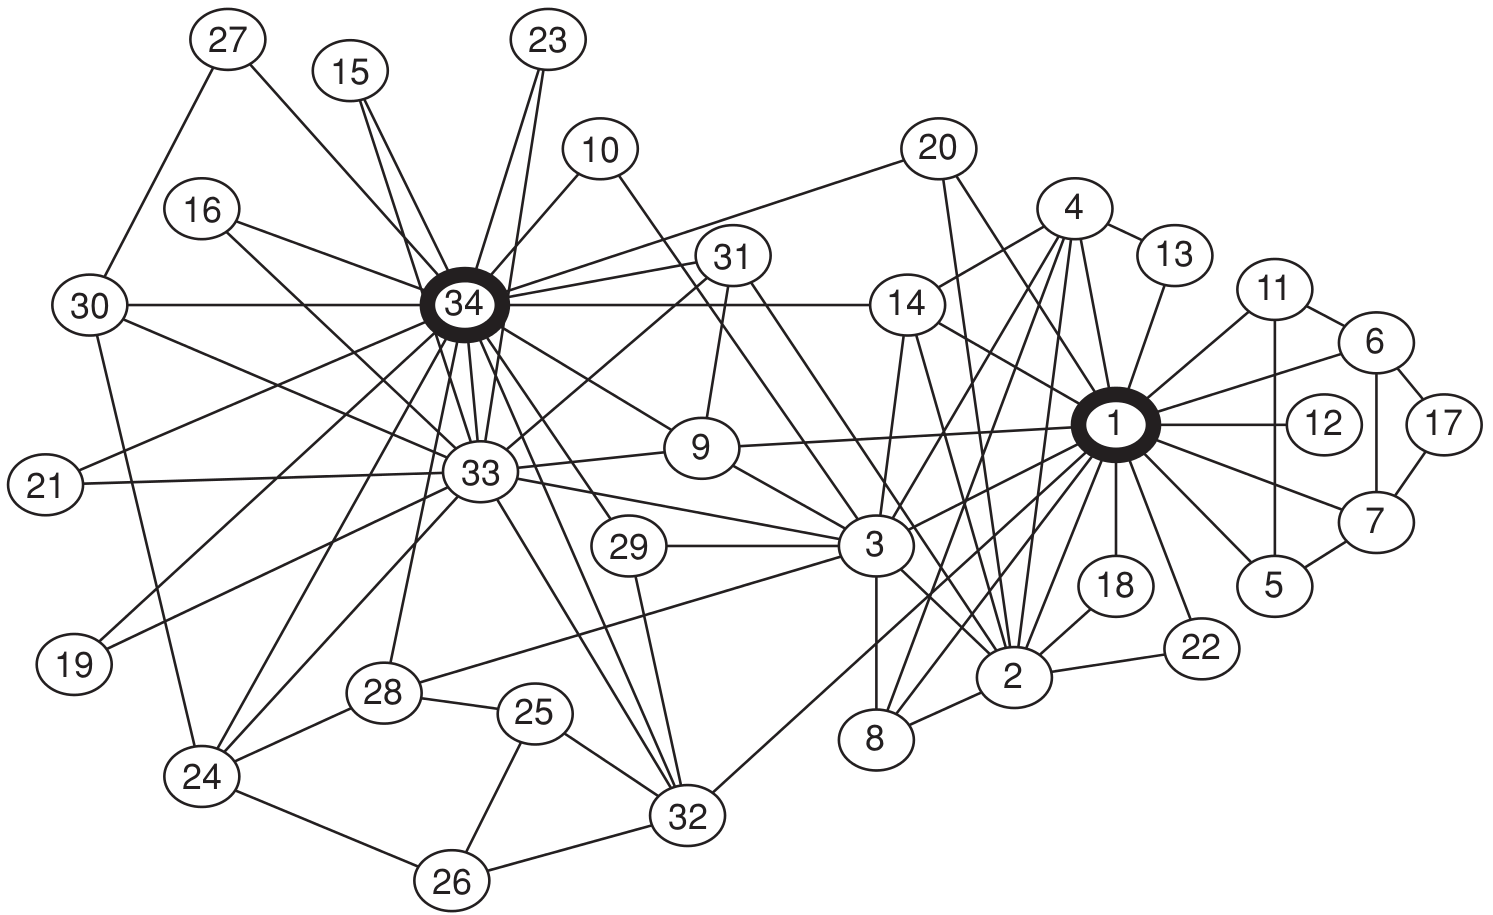
\includegraphics[width=0.75\linewidth]{images/17_karate_club.png}
\caption{Illustration des relations amicales entre 34 personnes dans un
    club de karaté. Chaque n\oe ud représente une personne et chaque lien,
    un lien d'amitié entre ces personnes. On constate que tout le monde
n'est pas ami avec tout le monde. Grâce à cette structure, on peut
déduire certaines choses, par exemple : deux personnes ont beaucoup de
liens d'amitié avec d'autres personnes, mais pas entre eux.}
\end{figure}
\end{center}

\begin{figure}[!ht]
\centering
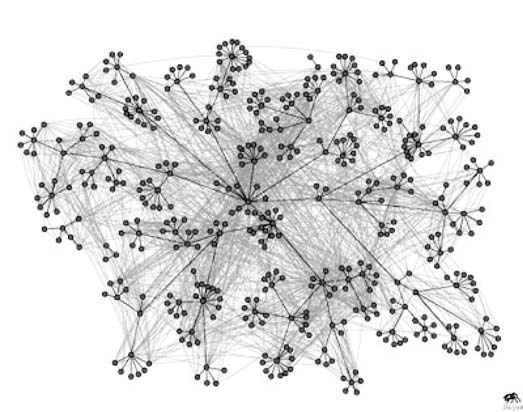
\includegraphics[width=0.75\linewidth]{images/social_networks_based_on_communication_and_interaction.png}
\caption{Des employés dans un laboratoire de recherche (n\oe ud) ont des
    liens entre eux : Lignes claires = communication e-mail. Lignes
    foncées = hiérarchie, organisation du laboratoire. On voit que la
    communication entre les gens suit relativement bien la structure
    hiérarchique, mais pas complètement. On peut voir comment les gens
collaborent, leurs degrés de collaboration, etc.}
\end{figure}

\begin{figure}[!ht]
\centering
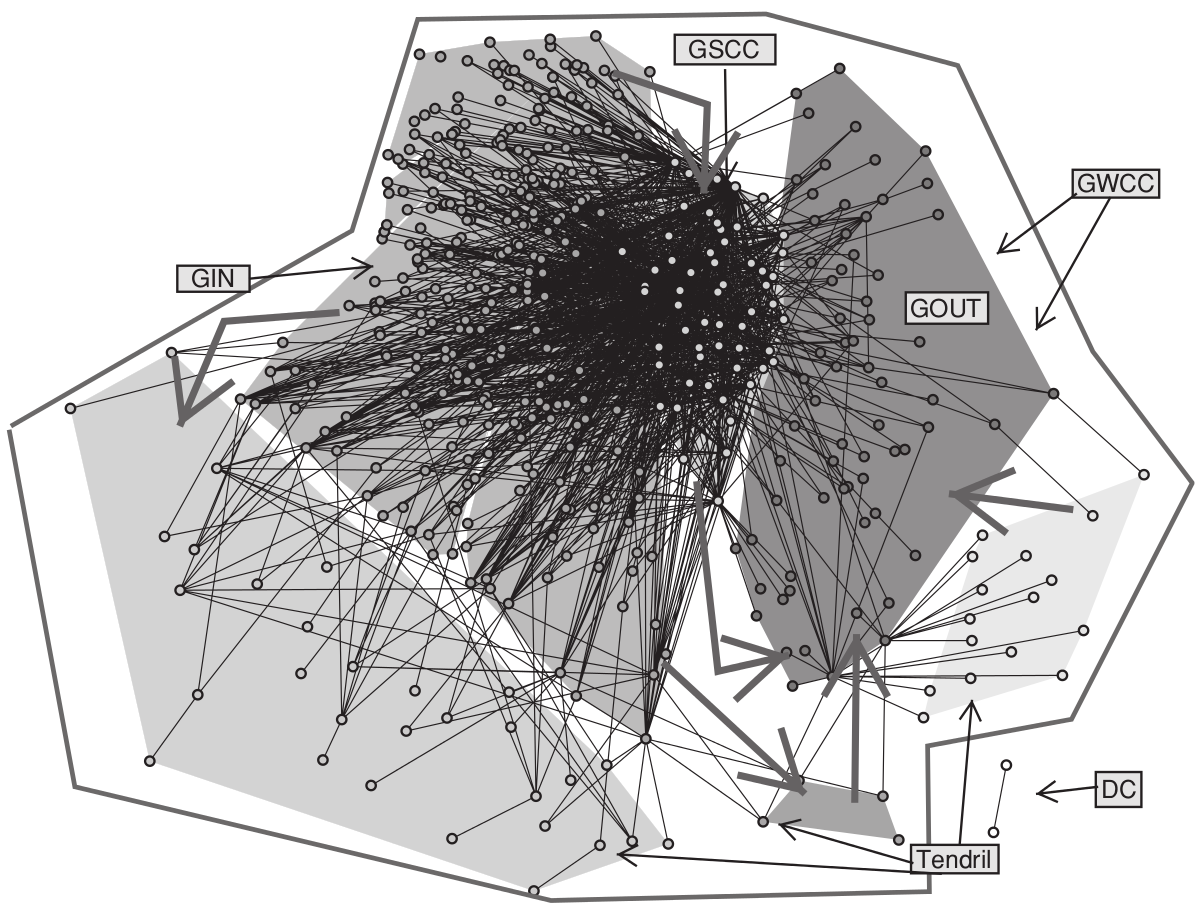
\includegraphics[width=0.65\linewidth]{images/reseaux_prets_entre_banques.png}
\caption{On constate que dans cette illustration, il y a beaucoup plus
    de nœuds. Chaque nœud est une institution financière (banque par
    exemple). Les liens représente des relations entre les banques,
    c'est à dire des prêts faits par une banque à une autre. Le graphe
    est connexe (il y a des chemins entre toutes les banques). Le centre
    est très dense, ça montre une faiblesse du système financier : si
    une banque dans le centre fait faillite par exemple, toutes les
    autres banques liées à elle sont également mises en danger . Donc si
    le noyau central est trop grand, c'est une faiblesse. En regardant
    cette structure, on peut trouver les faiblesses et les comprendre.
Ça peut être très important.}
\end{figure}

\begin{figure}[!ht]
\centering
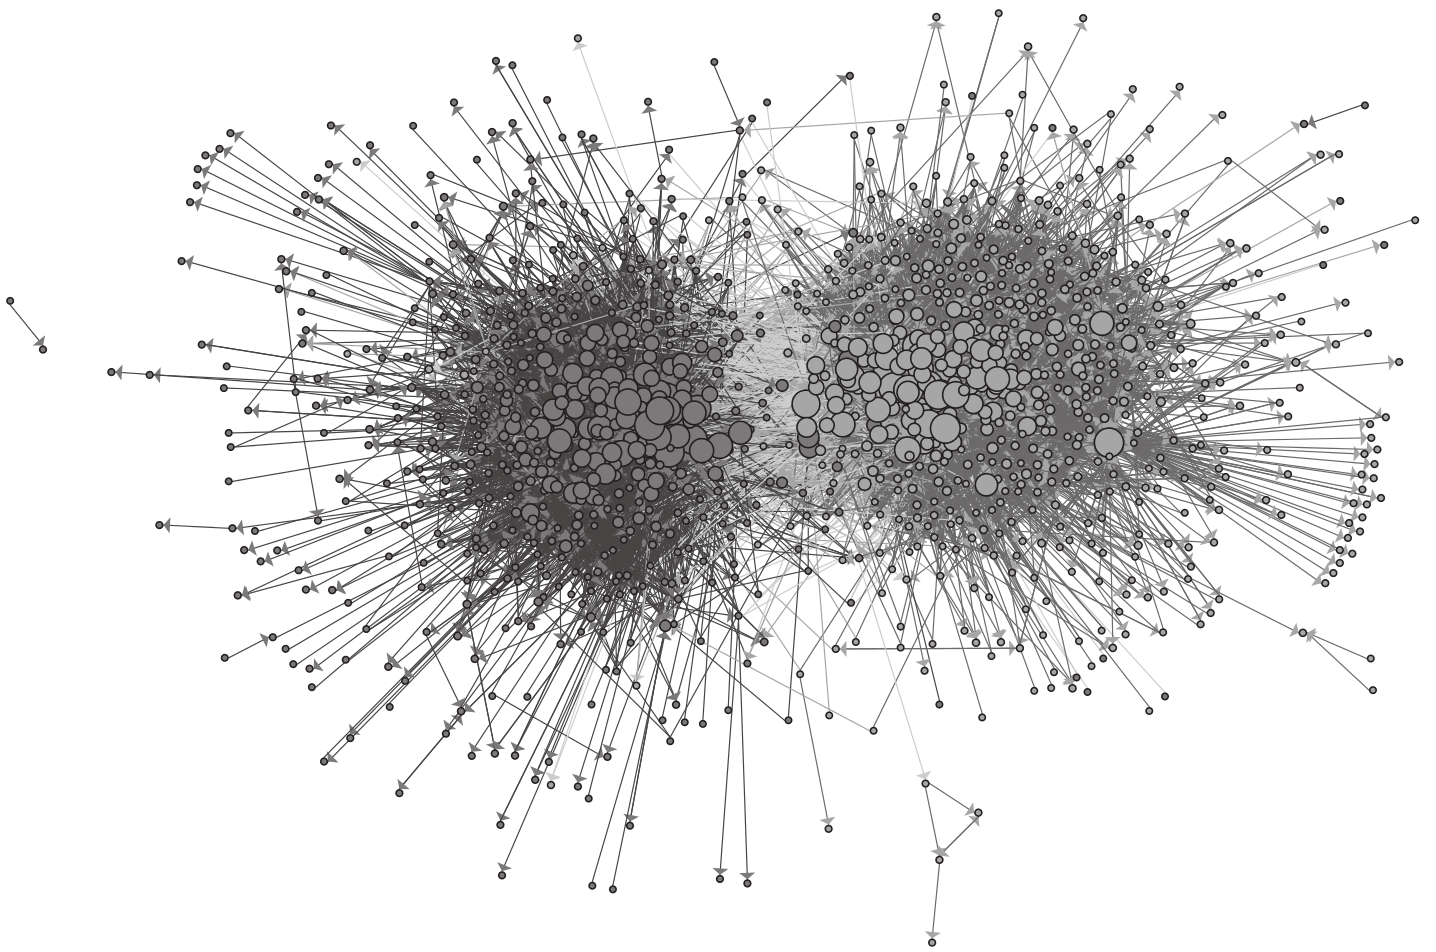
\includegraphics[width=0.65\linewidth]{images/network_structure_of_political_blogs.png}
\caption{Un n\oe ud représente un blog politique et un lien, une référence
    vers un autre blog. Nous avons deux partis qui représentent chacun
    un noyau : les démocrates et les républicains. On constate qu'il y a
    moins de connexions entre les deux noyaux qu'à l'intérieur de
    ceux-ci. On peut visualiser cette structure et se poser des
    questions : est-ce que cette absence de contact entre les deux
factions d'un monde bipolaire est un problème ?}
\end{figure}

Ce sont divers exemples que nous allons essayer d'analyser. Sur Internet, il y a beaucoup de nœuds avec de grandes capacités de calcul et de stockage. Grâce à de nouveaux outils utilisés sur internet pour analyser l'information, on peut observer la structure des graphes (ce qu'on ne pouvait pas faire avant).

\clearpage

\section{Introduction}
\begin{itemize}
\item Structure des réseaux (Facebook, Twitter, réseau économique,...).
\item Comportement des participants (interactions : chaque nœud sera un participant et va interagir).En principe, chaque nœud ne voit que son voisinage et interagit en conséquence.

\begin{itemize}
	\item Interactions \textit{locales} avec conséquences \textit{globales}.
	Il faut faire le lien entre ces deux choses.
	\item Effets non attendus. Par exemple les réseaux routiers : s'il y a des bouchons, on augmente la capacité du réseau (en ajoutant une voie). 
	Le résultat peut être contre intuitif, ça peut être :
	\begin{itemize} 
		\item Une réduction des transferts.
		\item Une augmentation du trafic. (résultat opposé à celui attendu)
	\end{itemize}	
	\item Le \textbf{Paradoxe de Braess} nous dit que l'ajout d'une nouvelle capacité à un réseau peut réduire la performance globale (effet non attendu).
Il faut donc comprendre comment le réseau fonctionne pour prévoir la réaction à une modification plutôt que d'agir impulsivement et avoir des effets non attendus.
\end{itemize}
\end{itemize}

\section{Nouvelle discipline}
Les graphes et leurs propriétés évoluent avec le temps, ce n'est pas statique.

Nouvelles disciplines pour analyser des graphes d'informations tirés de sites comme YouTube, Flicker, etc.

Synthèse de 3 disciplines :
\begin{enumerate}

	\item Mathématiques : théorie des graphes
	\item Mathématiques : théorie des jeux\\
		Exemple : YouTube impose ses règles, c'est le croupier, et ceux qui utilisent YouTube sont des joueurs.
	\item Sociologie : étude des groupes sociaux\\
		les participants sont humains ou guidés par un humain. Il n'est pas uniquement question de mathématiques, il faut aussi comprendre les humains.
\end{enumerate}

Dans ce cours, nous nous concentrerons principalement sur la théorie des graphes. La théorie des jeux sera abordée de façon intuitive, et nous parlerons un peu de la sociologie.

\subsection{Théorie des jeux}
On a un ensemble de participants qui jouent à "un jeu" (un ensemble de règles suivies par tous les participants). Chaque participant doit agir : 

\begin{itemize}
\item Simple à spécifier (comme les échecs : 2 participants et 1 action en alternance). 
\item Compliqué : pas d'alternance, tout le monde agit en même temps. C'est un système concurrent.
\end{itemize}

Exemple d'action simple : la vente aux enchères : 
	nombre fini de participants,
	règles simples et définies (différentes techniques sont possibles)
	
\vspace{1cm}

On va rester intuitif sur ce sujet, mais si on veut être plus précis, il y a des champs mathématiques qui étudient les systèmes concurrents.

Enfin, on peut aussi voir que la position dans le graphe peut aussi apporter des avantages.

\begin{itemize}
	\item \textbf{Figure 1.8} Réseau d'interaction économique entre pays. Structure de l'économie mondiale : Hong Kong a un gros avantage, il a une porte d'entrée vers la Chine (à l'époque). Certains pays sont des partenaires privilégie des États-Unis... 

\begin{figure}[!ht]
\centering
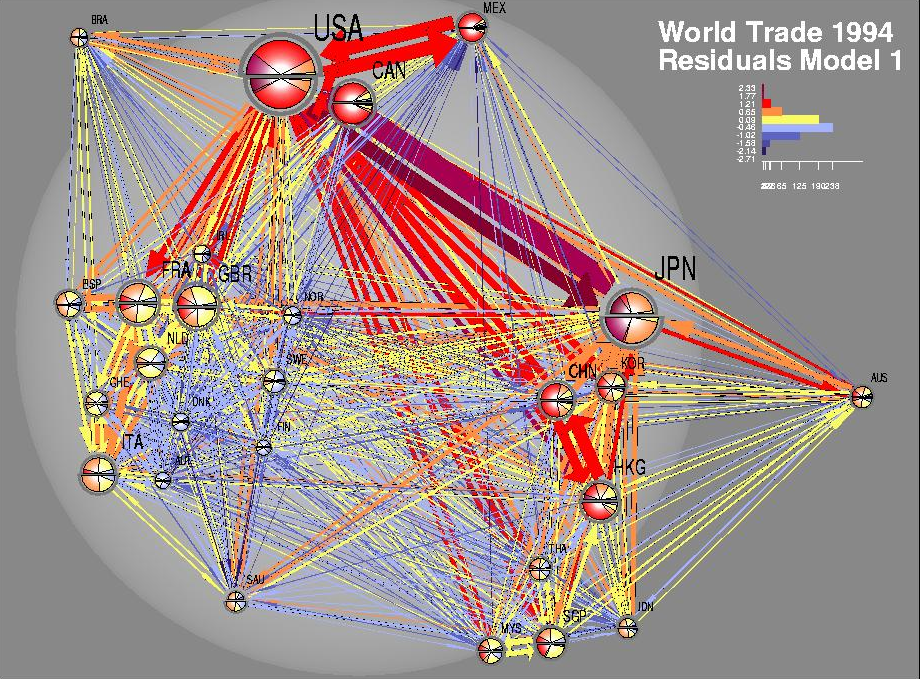
\includegraphics[width=0.8\linewidth]{images/network_international_trade.png}
\end{figure}

	\item \textbf{Figure 1.9} Chemins de commerces médiévaux en Europe. Une position stratégique donne des avantages. Tous ces avantages viennent de la structure du réseau (notons que le comportement d'un participant peut dépendre de la structure).
\begin{figure}[!H]
\centering
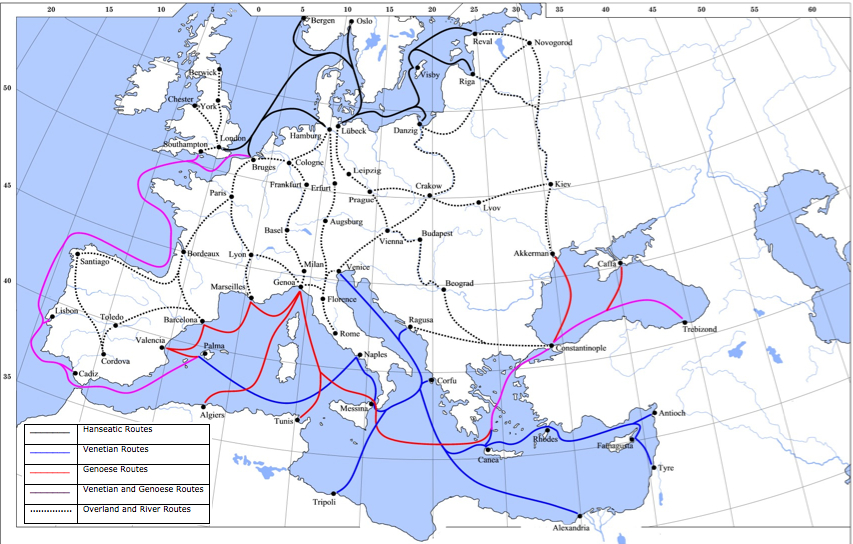
\includegraphics[width=0.9\linewidth]{images/map_of_medieval_trade_routes.png}
\end{figure}
\end{itemize}

Si on observe correctement le réseau, on peut se placer en position d'avantage et se mettre à une position qui donne plus de pouvoir.

Si on connaît la structure, une petite action peut suffire pour arrêter une épidémie en coupant les liens par lesquels cette épidémie pourrait se répandre.

  \chapter{Théorie des graphes}

\section{Définitions}
Un graphe G est un ensemble de liens et de nœuds. Un lien est une paire de deux nœuds.
\begin{center}
	G = (N,E)\\
	N = n\oe ud\\
	E = edge (lien, arête)\\
\end{center}

Deux types de graphes :

\begin{itemize}
\item \textbf{Les graphes orientés} (avec flèches et principe de direction). Une arête/lien est une paire de nœuds. L'ordre a de l'importance. Dans cet exemple, les paires de nœuds sont : (A,B), (A,C), (D,A) et (C,D). 

\begin{figure}[!ht]
\centering
\begin{tikzpicture}[line cap=round,line join=round,>=triangle 45,x=1.0cm,y=1.0cm]
\clip(4.5,4.) rectangle (9.,8.);
\draw [->] (8.02,5.58) -- (6.1,4.68);
\draw [->] (6.1,4.68) -- (5.24,6.72);
\draw [->] (5.24,6.72) -- (8.02,5.58);
\draw [->] (5.24,6.72) -- (7.4,7.28);
\begin{scriptsize}
\draw [fill=black] (5.24,6.72) circle (1.5pt);
\draw[color=black] (5.38,7.) node {$A$};
\draw [fill=black] (7.4,7.28) circle (1.5pt);
\draw[color=black] (7.54,7.56) node {$B$};
\draw [fill=black] (8.02,5.58) circle (1.5pt);
\draw[color=black] (8.16,5.86) node {$C$};
\draw [fill=black] (6.1,4.68) circle (1.5pt);
\draw[color=black] (6.12,4.48) node {$D$};
\end{scriptsize}
\end{tikzpicture}
\caption{Graphe orienté}
\end{figure}


\item \textbf{Les graphes non orientés} (sans flèche, sans direction).
    Une arête est un ensemble de deux n\oe uds. On ne parle pas de "paire"
    vu que l'ordre des nœuds n'a pas d'importance. Ici, parler de
    l'arête (A,B) ou (B,A) revient à la même chose.
\end{itemize}

\begin{figure}[!ht]
\centering
\begin{tikzpicture}[line cap=round,line join=round,>=triangle 45,x=1.0cm,y=1.0cm]
\clip(4.5,4.) rectangle (9.,8.);
\draw (7.4,7.28)-- (5.24,6.72);
\draw (5.24,6.72)-- (6.1,4.68);
\draw (6.1,4.68)-- (8.02,5.58);
\draw (8.02,5.58)-- (5.24,6.72);
\begin{scriptsize}
\draw [fill=black] (5.24,6.72) circle (1.5pt);
\draw[color=black] (5.38,7.) node {$A$};
\draw [fill=black] (7.4,7.28) circle (1.5pt);
\draw[color=black] (7.54,7.56) node {$B$};
\draw [fill=black] (8.02,5.58) circle (1.5pt);
\draw[color=black] (8.16,5.86) node {$C$};
\draw [fill=black] (6.1,4.68) circle (1.5pt);
\draw[color=black] (6.24,4.96) node {$D$};
\end{scriptsize}
\end{tikzpicture}
\caption{Graphe non orienté}
\end{figure}


\vspace{0.3cm}
Ce cours s'intéressera principalement aux graphes non orientés.

\section{Chemins et connectivité}
	Voici la définition des différents types de chemins dans un graphe :
	\begin{description}
	\item [Chaine] : Dans un graphe non orienté, une chaîne reliant un sommet $x$ à un sommet $y$ est une suite finie d'arêtes consécutives, reliant $x$ à $y$
	\item[Chemin]: séquence de n\oe uds dont chaque paire consécutive est reliée par une arête.
    	\item[Chemin simple]: c'est un chemin dont chaque n\oe ud se trouve au maximum une fois dans la séquence de n\oe uds.
    	\item[Cycle]: c'est un chemin dont le premier et le dernier n\oe ud sont les mêmes. Un cycle possède au moins 3 liens (arêtes).\\
	\end{description}

Une fois la notion de chemin connue, on peut définir la notion de connectivité d'un graphe.
	\begin{description}
    	\item[Connectivité]: un graphe est dit connexe si pour toutes paires de n\oe uds A et B, il existe au moins un chemin de A vers B.\\
	\end{description}

Il existe des graphes qui ne sont pas connexes. La figure \ref{graphe_non_connexe} montre un exemple de graphe non connexe.

	\begin{figure}[!h]
	\center
	\includegraphics[scale=0.3]{images/18_graphe_non_connexe.png}
	\caption{\label{graphe_non_connexe} Graphe non connexe}
	\end{figure}
	
Ce graphe possède deux composants, $AB$ et $CDE$. Ces composants sont les parties connexes du graphe. On ajoute donc deux définitions pour les composants.
	\begin{description}
    \item[Composant d'un graphe]: c'est un sous-graphe (partie de graphe) qui est connexe. Il est maximal s'il ne fait pas partie d'un composant plus grand.
    \item[Composant géant] : il s'agit d'un composant qui contient une fraction significative de l'ensemble des n\oe uds contenus dans le graphe.
    \end{description}
    
    Par exemple, le graphe des amitiés mondiales n'est sûrement pas connexe. En effet, il peut y avoir des habitants d'une île reculée qui se connaissent entre eux, mais qui n'ont pas de connexion avec le reste du monde. Il peut aussi y avoir un seul individu asocial qui n'ai pas d'ami et forme un composant à lui seul. Cependant, la majorité du monde est connectée; on a donc un énorme composant géant.
    
    \vspace{1ex}
    C'est une propriété générale des grands graphes complexes: il est rare qu'ils soient connexes, mais ils ont très souvent un composant géant. Avoir plusieurs composants géants est instable: il arrive vite qu'un lien se forme entre les deux composants, formant ainsi un seul composant géant. Si avant le \textsc{xv}\textsuperscript{ème} siècle, il y avait un composant géant eurasien et un autre Américain, il n'a fallu qu'un lien (la découverte de l'Amérique par Christophe Colomb) pour assembler les deux composants, avec toutes les conséquences que cela a entraîné (maladies, exploitation, etc.).
    		
    \vspace{1ex}
    
	\begin{figure}[!h]
	\center
	\includegraphics[scale=0.3]{images/18_gr_connexe.png}
	\caption{\label{gr_connexe} Graphe connexe}
	\end{figure}
	
	Avec les éléments que nous venons de définir, on est en mesure d'analyser tout un graphe. On peut le partitionner en composants et regarder la structure interne de chacun d'entre eux. Par exemple, dans la figure \ref{gr_connexe}, on peut partitionner en deux composantes, $ABC$ et $DEF$. On constate que le lien $CD$ est un lien spécial, car si on l'enlève, il déconnecte le graphe en deux composants distincts.

	

\section{Distance entre n\oe uds}
Nous allons maintenant définir la longueur d'un chemin ainsi que la distance entre deux n\oe uds :
\begin{description}
\item[Longueur d'un chemin] : le nombre d'arêtes consécutives sur ce chemin.
\item [Distance entre deux n\oe uds] : le chemin le plus court entre ces deux n\oe uds.
\end{description}

La méthode de calcul de distance entre deux n\oe uds est la traversée en largeur d'abord (\emph{breadth-first traversal}). Cela consiste à débuter par un n\oe ud, puis à regarder tous les n\oe uds qui sont à une distance de 1 du n\oe ud de départ. À partir de tous ceux-là, on regarde les n\oe uds qui sont adjacents, et donc à une distance 2 du n\oe ud de départ. On continue jusqu'à arriver au n\oe ud d'arrivée. On a donc, à chaque étape, constitué des couches de n\oe uds se trouvant à une certaine distance. Cet algorithme sera expliqué plus en détail par après.

\section{Phénomène du petit monde}
Le « phénomène du petit monde », aussi connu sous le vocable « paradoxe de Milgram » (du nom du psychosociologue  \textit{Stanley Milgram}), est l'hypothèse que chacun puisse être relié à n'importe quel autre individu par une courte chaîne de relations sociales. La figure \ref{petit_monde} montre la probabilité qu'ont deux personnes d'être reliés par $x$ intermédiaires. 
	\begin{figure}
	\center
	\includegraphics[scale=0.5]{images/18_fig.png}
	\caption{\label{petit_monde} Statistiques du phénomène du petit monde}
	\end{figure}
Cette  courte chaîne de relations sociales a été approfondie par la théorie des « six degrés de séparation » affirmant qu'en prenant deux personnes, il est possible de trouver une chaîne d'amis entre eux de taille maximum 6.
Différents types de distances entre des personnes existent, comme:
	\begin{itemize}
	\item Le nombre d'Erdös est la distance de collaboration avec le célèbre mathématicien  \textit{Paul Erdös} qui a réalisé de très nombreuses co-publications. Avoir réalisé une publication en collaboration avec Erdös correspond au nombre d'Erdös 1. Avoir écrit une publication avec quelqu'un qui a co publié avec Erdös équivaut au nombre 2, etc. \footnote{xkcd.com/599/}
	\item Le nombre de Bacon est la distance de collaboration dans un film avec l'acteur  \textit{Kevin Bacon}.
	\end{itemize}
Ce phénomène de petit monde est particulièrement vrai pour les réseaux créés dynamiquement. Nous expliquerons plus en détail pourquoi cette affirmation est vraie dans la suite du cours.

\section{Liens forts et faibles}

Un réseau peut évoluer de différentes manières et selon différents mécanismes.
Considérons un exemple où chaque n\oe ud correspond à une personne et les arcs correspondent à un lien d'amitié (figure \ref{fermeture_triadique}).
	\begin{figure}[!h]
	\center
	\includegraphics[scale=0.5]{images/18_fermeture_triadique.png}
	\caption{\label{fermeture_triadique} Exemple de fermeture triadique}
	\end{figure}
Dans cet exemple, on voit que $A$ est ami à la fois avec $B$ et avec $C$. Dans cette condition, il est fort probable que $B$ et $C$ deviennent eux-mêmes amis. C'est ce qu'on appelle la fermeture triadique.

\textbf{Propriété de fermeture triadique forte} : si A a un lien fort avec B et avec C, alors un lien au moins faible va se créer entre B et C.

Cette situation nous amène à nous intéresser à la notion de coefficient de regroupement qui reflète la probabilité qu'un arc se crée entre deux n\oe uds dans un graphe dynamique. 
Dans l'exemple ci-dessus, cela correspondrait au fait que $C$ et $B$ deviennent amis. On peut démontrer qu'au plus on fait de fermetures triadiques, au plus le coefficient de regroupement est élevé.

\subsection*{Exemple}
Une étude a été faite dans les années 1960, par le sociologue américain \textit{Mark Granovetter}, dans laquelle il s'est intéressé aux personnes qui changent de travail et plus particulièrement à la manière dont ils trouvent un nouveau travail. Il a remarqué que les personnes trouvent du travail plutôt via des connaissances que via des amis. Cela s'explique par la structure des graphes des amis et nous amène à définir les notions de \textbf{liens forts} et de \textbf{liens faibles} (figure \ref{liens_forts_et_faibles}). Nous reviendrons sur cet exemple plus tard.

	\begin{figure}[!h]
	\center
	\includegraphics[scale=0.25]{images/18_liens_forts_et_faibles.png}
	\caption{\label{liens_forts_et_faibles} Liens forts et faibles}
	\end{figure}

    
\section{Ponts}
Pour expliquer l'exemple précédent, nous avons besoin de la notion de pont (figures \ref{Pont} et \ref{Pontlocal}).
	\begin{description}
	\item[Pont] Un lien entre $A$ et $B$ est un pont si l'enlèvement de ce lien aboutit à la séparation du graphe en deux composants disjoints.
    \item[Pont local] Un lien entre $A$ et $B$ est un pont local si l'enlèvement de ce lien aboutit au fait que deux composantes sont reliées par un chemin significativement plus long.
    \end{description}
    
    \begin{figure}[ht]
    \center
    \includegraphics[scale=0.25]{images/18_Pont.png}
    \caption{\label{Pont} Pont}
    \end{figure}
    
    \begin{figure}[ht]
    \center
    \includegraphics[scale=0.3]{images/18_Pontlocal.png}
    \caption{\label{Pontlocal} Pont local}
    \end{figure}

  Reprenons l'exemple de la figure \ref{liens_forts_et_faibles}, si l'on s'intéresse à la personne
A, on sait que s'il cherche du travail c'est fort probable que ce soit
via B qu'il en trouve (B est une connaissance de A). Sociologiquement, on sait que si deux amis ont un ami en commun, il y a des chances qu'ils deviennent ami aussi ou tout du moins connaissance (propriété de fermeture triadique forte). On peut donc en déduire que chaque pont local est tel que le pont entre A et B dans la figure 9.9 sera un lien faible (conséquence de la propriété de fermeture triadique forte).

En effet si le lien entre A et B était fort, la propriété de fermeture triadique forte nous dirait que d'autres liens se formeraient. Par exemple, entre E et B et entre A et F ce qui aurait pour conséquence que le lien A-B ne serait plus un pont.B fourni donc de nouvelles informations à A via le pont local.

\section{Force d'un lien dans un grand réseau}
Pour caractériser la force d'un lien dans un grand réseau, il va falloir généraliser les concepts relatifs aux liens forts et faibles vus précédemment.
La force d'un lien sera caractérisée en y attribuant une quantité numérique, on va utiliser la notion de chevauchement de voisinage (neighbourhood overlapping) pour ça.
\begin{center}
Chevauchement de voisinage = $\frac{\text{Nombre de noeuds voisins de A \textbf{et} B}}{\text{Nombre de noeuds voisins de A \textbf{ou} B}}$.\\
\end{center}
La quantité numérique augmentera en fonction de ce chevauchement. Plus cette valeur de chevauchement de voisinage tendra vers 0, plus ce lien deviendra un pont local.
\newline
\section{Force des liens en pratique dans un réseau téléphonique}
Une étude portée sur les conversations cellulaires nous prouve que plus les liens entre des individus sont fort, plus ces personnes passeront du temps au téléphone à communiquer. Effectivement, on remarque que la durée augmente au fur et à mesure que le chevauchement de voisinage augmente.
\newline

\section{Force des liens en pratique sur Facebook}
Facebook est un réseau social développé sur internet permettant à des individus de communiquer avec des personnes de leur entourage.
Les liens entre individus sur Facebook sont nommés les liens d'amitié.
Facebook est ainsi notamment un bon exemple où la force des liens est utilisée au maximum.
D'après une étude réalisée sur une période d'un mois, on trouve trois catégories de liens sur Facebook, caractérisant soit:
\begin{itemize}
\item une communication réciproque.
\item une communication orientée.
\item une relation maintenue.
\end{itemize}
On peut faire une comparaison avec la force d'un lien, le nombre de personnes ayant un lien d'amitié avec quelqu'un augmente en fonction de la taille du voisinage. 
Les observations montrent aussi que la propagation d'informations est plus rapide avec la 3e catégorie de lien.
\newline

\section{Twitter}
Twitter est un microblog qui permet de partager de petits messages (140 caractères au maximum). Il est basé sur une relation de Followers à Followees.
Force du lien :
\begin{itemize}
\item Faible si on est follower.
\item Forte si on envoie un message ciblé.
\end{itemize}
Si on "suit" plus de personnes, on a plus d'amis (jusqu'à un certain point, on suit une courbe logarithmique). Effectivement, cela s'explique par le fait que pour entretenir des liens forts, ceci demande un effort conditionnel. Il y a une limite physique aux nombres de liens forts que l'on peut posséder. A contrario, il ne demande pas de temps ou d'effort pour 'suivre' quelqu'un. Il y a moins de contraintes, c'est un engagement passif et c'est ce qui est prôné sur Twitter.

  \section{Notion de trou structurel et capital social}
Comme nous l'avons vu précédemment, il existe deux types différents de liens. Les liens faibles et les liens forts, ces derniers étant beaucoup moins nombreux que les faibles.

Or lorsque l'on regarde un réseau, les noeuds ont aussi une grande importance. En fonction de la structure ou de l'organisation du graphe, certains noeuds posséderont quelques avantages et inconvénients. 
Par la suite, nous allons montrer que cette propriété propre aux noeuds est de posséder un "pouvoir".

\subsection{L'enchâssement d'un lien (embeddedness)}
Attardons-nous tout d'abord à l'enchâssement d'un lien, c'est-à-dire le
nombre de voisins commun entre les deux noeuds de ce lien. Par ailleurs,
on peut observer que ce nombre est équivalent au numérateur du c\oe fficient de chevauchement.
On peut dire qu'un lien est plus fortement incrusté dans le réseau si les 2 noeuds du lien possèdent un grand nombre de voisins. 

Considérons le graphe~\ref{graph:graphe1} à la page~\pageref{graph:graphe1}. On peut remarquer que le noeud \textbf{A} admet quelques fermetures triadiques parmi ses voisins tandis que le noeud \textbf{B} permet au \textbf{réseau 1} de rejoindre les deux autres.

\begin{figure}[h]
\centering
\begin{tikzpicture}[scale=0.75]
\coordinate (2) at (0,2);
\coordinate (3) at (1,0);
\coordinate (1) at (2,3);
\coordinate (4) at (3,0);
\coordinate (B) at (4,2);
\coordinate (A) at (2,1.5);
\coordinate (C) at (7,3);
\coordinate (D) at (7,0);

\draw (1) node{$\bullet$};
\draw (2) node{$\bullet$};
\draw (3) node{$\bullet$};
\draw (4) node{$\bullet$};
\draw (B) node[above right]{B} node{$\bullet$};
\draw (A) node[below]{A} node{$\bullet$};
\draw (C) node[above left]{C} node{$\bullet$};
\draw (D) node[below left]{D} node{$\bullet$};

\draw[thick] (1)--(2)--(3)--(4)--(B)--(1);
\draw[thick] (A)--(1);\draw[thick] (A)--(2);\draw[thick] (A)--(4);\draw[thick] (A)--(B);
\draw[thick] (B)--(C); \draw[thick] (B)--(D);
\draw[dashed] (C)--(7,4);\draw[dashed] (C)--(8,3);\draw[dashed] (C)--(7,4); \draw[dashed] (7,4)--(8,4);\draw[dashed] (8,4)--(8,3);\draw[dashed] (8,3)--(7,4);
\draw[dashed] (D)--(8,0);\draw[dashed] (D)--(8,-1);\draw[dashed] (D)--(7,-1);\draw[dashed] (8,0)--(8,-1)--(7,-1)--(8,0);

\draw[dotted, rounded corners=5pt, thick] (-1,-1) rectangle (5,4);
\node[draw,dotted, thick,rectangle, rounded corners=2pt] (R1) at (0.2,-1.5) {réseau 1};

\draw[dotted, rounded corners=5pt, thick] (6,-2) rectangle (9,5);
\node[draw,dotted, thick,rectangle, rounded corners=2pt] (R1) at (10.75,3) {autres réseaux};

\end{tikzpicture}
\caption{Un réseau central lié à deux autres sous-réseaux}
\label{graph:graphe1}
\end{figure}

On peut aussi apercevoir que le noeud \textbf{A}  est localisé là où le coefficient de regroupement est assez élevé contrairement à \textbf{B} qui est dans une zone à faible densité . On dit que les liens de \textbf{A} sont 'incrustés', ils ont un enchâssement significatif. 

Deux individus connectés par un lien possédant un grand enchâssement  auront une plus grande confiance mutuelle. En plus de la simple force du lien, c'est également la structure du réseau qui va augmenter la confiance entre deux nœuds. Il y aura une observation mutuelle, une surveillance de la part des amis communs aux deux nœuds.
Une représentation de ce concept est donnée dans le graphe ~\ref{graph:graphe2}. Dans cette figure, une observation mutuelle entre \textbf{A} et \textbf{B} est de mise.

\begin{figure}[h!]
\centering
\begin{tikzpicture}
\coordinate (A) at (0,0);
\coordinate (B) at (4,0);


\draw (B) node[right]{B} node{$\bullet$};
\draw (A) node[left]{A} node{$\bullet$};
\node[draw,circle,dotted] (P1) at (2,1){P1};
\node[draw,circle,dotted] (P2) at (2,-1){P2};

\draw (A)--(B);

\draw (A) to[bend left] (P1.north west) (P1.north east) to[bend left](B);
\draw (A) edge[out=20, in=-120] (P1.south west) (P1.south east) edge[out=-60, in=160] (B);

\draw (A) edge[out=-20,in=120] (P2.north west) (P2.north east) edge[out=60,in=-160](B);
\draw (A) to[bend right]  (P2.south west) (P2.south east) to[bend right] (B);

\end{tikzpicture}
\caption{Deux noeuds possédant un enchâssement significatif}
\label{graph:graphe2}
\end{figure}

 En effet, imaginons que le noeud \textbf{A} effectue une action quelconque, tous les autres noeuds (par exemple, ceux de \textit{P1} et \textit{P2}) peuvent voir cette action.
Ainsi, deux noeuds possédant un enchâssement suffisamment conséquent ont une certaine confiance mutuelle.

On peut donc en tirer la propriété suivante provenant directement de la structure du graphe :

\vspace{1ex}
\textit{Plus l'enchâssement augmente, plus la confiance mutuelle est grande.}

\vspace{1ex}
En conséquence, \textbf{A} possède une grande influence car il a une forte confiance mutuelle avec tous ses amis.

Revenons maintenant au graphique \ref{graph:graphe1}. Bien que le lien \textbf{A} possède un grand enchâssement, il n'en est pas de même pour \textbf{B} avec \textbf{C} et \textbf{D}.
En effet, ils ne peuvent pas avoir une confiance mutuelle, car les autres noeuds de leur réseau respectif ne peuvent plus les "observer".

\vspace{1ex}
Bien que d'un certain point de vue, \textbf{A} pourrait posséder plus d'avantages que \textbf{B} grâce à ses fermetures et son voisinage, ce n'est pas tout à fait exact. Le noeud \textbf{B} possède lui aussi des avantages aussi fondamentaux que \textbf{A}.

\vspace{1ex}
\begin{itemize}
\item \textbf{B} est au bord d'un pont local. Il joue le rôle d'intermédiaire entre plusieurs réseaux.
\item \textbf{B} s'étend sur un trou structurel, il remplit le vide entre plusieurs ensembles de noeuds.
\item \textbf{B} est le seul lien pour communiquer avec certains ensembles. Tous les chemins entre ces deux communautés passent par \textbf{B}. Il est donc incontournable.
\item Il a des informations dispersées auxquelles les autres n'ont pas accès. Il va donc pouvoir amplifier sa créativité en observant les informations ou en en faisant passer certaines pour siennes.\footnote{Le fait d'être présent sur un pont pour pouvoir espionner efficacement peut par exemple être observé dans les programmes de surveillance de la NSA (États-Unis) ou du GCHQ (Grande-Bretagne) qui profitent du pont internet entre l'Europe et l'Amérique.}
\item Il joue le rôle de gardiennage social, il peut réguler l'accès de l'extérieur.
\end{itemize}

Par ailleurs, ces quelques derniers avantages peuvent engendrer un conflit d'intérêts entre \textbf{B} et ses sous-ensembles. Par exemple, dans le cas où \textbf{B} voudrait laisser deux réseaux scindés alors que ceux-ci désireraient s'assembler.\\

$\Rightarrow$ On fait donc appel à des notions de \textit{pouvoir} ou d'\textit{avantage}.\\

Ces notions sont aussi appelées \textit{capital social} ou capacité à se procurer des avantages grâce à l'appartenance à une structure sociale.

%Sur ce graphe distinguons les noeuds adjacents A et B.
%A: 
%- plus de confiance grâce à la fermeture dans son voisinage.
%
%B a d'autres avantages qui sont aussi fondamentaux:
%- B est au bord d'un pont local. Il joue le rôle d'intermédiaire entre plusieurs communautés.
%- B s'étend sur un trou structurel, il rempli le vide entre plusieurs ensembles de noeuds. 
%- B est le seul lien pour communiquer avec certains ensemble. En fait, tous les chemins entre ces deux %communautés passent par B. 
%- B a des informations dispersées auxquelles les autres n'ont pas accès. C'est un amplificateur de créativité.

\subsection{Notion de capital social}
Le capital social est la capacité à se procurer des avantages grâce à l'appartenance à une structure sociale. C'est une forme de capital, car elle représente une capacité que l'on possède et que l'on peut utiliser.  
Il existe d'autres notions de capitaux:\\

\begin{itemize}
\item Capital physique (exemple : technologie ) 
\item Capital humain (exemple : expertise des personnes )
\item Capital économique (exemple : monétaire ) 
\item Capital culturel (exemple : les ressources accumulées dans une culture, les connaissances communes )
\end{itemize}

\section{Similitude des noeuds}
Après nous être intéressés aux liens entre les noeuds, nous allons nous concentrer sur les similitudes entre  ces noeuds. 

\subsection{Principe de similitude}
La notion sociologique de similitude s'observe par une augmentation du nombre de liens entre les noeuds. 
Exemple: Les étudiants de l'UCL présentent une similitude par le fait qu'ils font partie de la même université. 

Ce principe implique de nouveaux mécanismes dans la manière où nous allons représenter les graphes:

\begin{tabular}{lcp{7cm}}
Sélection & $\longrightarrow$ & \textit{local} (Chacun choisi ses amis) \\
Influence sociale & $\longrightarrow$ & \textit{global/extérieur} (Induite par les gens que l'on fréquente)
\end{tabular}

Exemple de la propriété d'influence sociale :\\ Le fait d'être dans le même auditoire qu'un autre individu peut constituer un lien dans le graphe.

Bien que la sociologie est un concept difficile à formaliser. 
Une idée pourrait être d'inclure les facteurs de similitudes dans le graphe.

\begin{figure}[!h]
\centering
\begin{tikzpicture}
\coordinate (Dan) at (0,0);
\coordinate (An) at (0,2);
\coordinate (lit) at (3,2);
\coordinate (kar) at (3,0);


\node[draw,circle] (Dan) at (Dan){Daniel};
\node[draw,circle] (An) at (An){Anna};
\node[draw] (kar) at (kar){club karaté};
\node[draw] (lit) at (lit){club littéraire};

\draw  (An)--(lit);
\draw (An)--(kar);
\draw (Dan)--(kar);

\end{tikzpicture}
\caption{Exemple d'un graphe personnes-intérêts}

\label{graph:graphe3-1}
\end{figure}


Les graphes sont maintenant constitués à partir de deux types de noeuds:
\begin{itemize}
\item noeud Individu : représente une personne physique.
\item noeud Focus : activité ou centre d'intérêt.
\end{itemize}

Mais aussi de deux types de liens:
\begin{itemize}
\item liens Personnes - Personnes
\item liens Personnes - Focus
\end{itemize}

Ces graphes aussi appelés réseau d'affiliations ont une caractéristique bien particulière, ils sont toujours bipartis.

\vspace{1ex}
Définition \textit{graphe biparti}: Soit un graphe G=G(V,E) et $V_{1}$, $V_{2}$ deux ensembles de noeuds et $ V_{1} \cup V_{2} = V $, un graphe est dit biparti s'il n'existe pas d'arête interne dans ces deux sous-ensembles.\\ $ \forall e = (u,v)\in E, u \in V_{1}$ et $v \in V_{2} $.

\vspace{1ex}
Le graphe ci-dessous représente l'affiliation des personnes (A, B, C, D) au conseil d'administration de différentes entreprises.
Comme on peut le voir (graphe \ref{graph:grapheGoogle}), il peut y avoir un conflit d'intérêts, par exemple entre Google et Apple. En effet, les deux compagnies sont concurrentes (sur le marché des smartphones), et pourtant une personne est membre des deux conseils d'administration.

\begin{figure}[h!]
\centering
\begin{tikzpicture}
\coordinate (D) at (0,0);
\coordinate (C) at (0,1);
\coordinate (B) at (0,2);
\coordinate (A) at (0,3);

\coordinate (Dis) at (4,0);
\coordinate (Ap) at (4,1);
\coordinate (Go) at (4,2);
\coordinate (Am) at (4,3);

\node[draw,circle] (D) at (D){D};
\node[draw,circle] (C) at (C){C};
\node[draw,circle] (B) at (B){B};
\node[draw,circle] (A) at (A){A};

\node[draw] (Dis) at (Dis){Disney};
\node[draw] (Ap) at (Ap){Apple};
\node[draw] (Go) at (Go){Google};
\node[draw] (Am) at (Am){Amazon};

\draw (A)--(Am);
\draw (A)--(Go);
\draw (B)--(Go);
\draw (C)--(Go);
\draw (C)--(Ap);
\draw (D)--(Ap);
\draw (D)--(Dis);

\end{tikzpicture}
\caption{Exemple d'un graphe représentant un conseil d'administration}

\label{graph:grapheGoogle}
\end{figure}

Par ailleurs, ces graphes bipartis ne sont pas statiques. En effet, ils peuvent subir des évolutions dans le temps comme des ajouts de noeuds, points d'intérêts, nouveaux liens ...\\

Ainsi, ces graphes nous fournissent plus de précisions que les précédents. 
Grâce à ce concept, on peut voir plus efficacement les changements et transformations lors d'évolutions.

\subsection{Nouveaux mécanismes de fermeture}
Nous avons déjà vu précédemment le principe de fermeture triadique.\\

\begin{figure}[h!]
\centering
\begin{tikzpicture}
\coordinate (A) at (0,1);
\coordinate (B) at (1,0);
\coordinate (C) at (2,1);


\node[draw,circle] (A) at (A){P};
\node[draw,circle] (B) at (B){P};
\node[draw,circle] (C) at (C){P};

\draw  (A)--(B);
\draw [dashed] (A)--(C);
\draw (C)--(B);

\end{tikzpicture}
\caption{Rappel de fermeture triadique}

\label{graph:graphe3}
\end{figure}

Grâce à la prise en compte des points d'intérêts (focus), deux nouveaux principes de fermeture peuvent être considérés:

\subsubsection{Fermeture focale}
\begin{figure}[h!]
\centering
\begin{tikzpicture}
\coordinate (A) at (0,1);
\coordinate (B) at (1,0);
\coordinate (C) at (2,1);


\node[draw,circle] (A) at (A){P};
\node[draw] (B) at (B){F};
\node[draw,circle] (C) at (C){P};

\draw  (A)--(B);
\draw [dashed] (A)--(C);
\draw (C)--(B);

\end{tikzpicture}
\caption{Exemple de fermeture focale}

\label{graph:graphe3}
\end{figure}

Comme on peut le voir sur le graphique~\ref{graph:graphe3}, deux personnes ayant des similitudes ou mêmes centres d'intérêts, peuvent devenir amis.

\subsubsection{Fermeture d'adhésion}
De la même manière, une personne ayant une activité peut convertir son ami.
\begin{figure}[h!]
\centering
\begin{tikzpicture}
\coordinate (A) at (0,1);
\coordinate (B) at (1,0);
\coordinate (C) at (2,1);


\node[draw,circle] (A) at (A){P};
\node[draw,circle] (B) at (B){P};
\node[draw] (C) at (C){F};

\draw  (A)--(B);
\draw [dashed] (A)--(C);
\draw (C)--(B);

\end{tikzpicture}
\caption{Exemple de fermeture d'adhésion}
\label{graph:graphe4}
\end{figure}

Ces deux nouveaux mécanismes de fermeture permettent de raisonner beaucoup plus fort sur ces graphes. Ils sont même essentiels ! Si on ne les prenait pas en compte, on ne pourrait jamais comprendre pourquoi un lien apparaît spontanément.

\vspace{1ex}
Ci-dessous, un exemple illustrant cette propriété:

\vspace{1ex}
Sans les concepts introduits dans cette partie, voici ce que l'on observerait:

\begin{figure}[h!]
\centering
\begin{tabular}{ccc}
\begin{tikzpicture}
\coordinate (A) at (0,0);
\coordinate (C) at (1.5,0);

\node[draw,circle] (A) at (A){P};
\node[draw,circle] (C) at (C){P};

\end{tikzpicture}
& \raisebox{2ex}{$\qquad \longrightarrow \qquad$}
\begin{tikzpicture}
\coordinate (A) at (0,0);
\coordinate (C) at (1.5,0);

\node[draw,circle] (A) at (A){P};
\node[draw,circle] (C) at (C){P};
\draw[dashed] (A)--(C);

\end{tikzpicture}
\end{tabular}
\caption{Apparition spontanée d'un lien}
\label{graph:graphe5}
\end{figure}

Heureusement avec la propriété de fermeture focale, on peut raisonner sur la raison de cette apparition.

\begin{figure}[!h]
\centering
\begin{tabular}{ccc}
\begin{tikzpicture}
\coordinate (A) at (0,0);
\coordinate (B) at (0.75,-1);
\coordinate (C) at (1.5,0);

\node[draw,circle] (A) at (A){P};
\node[draw] (B) at (B){F};
\node[draw,circle] (C) at (C){P};
\draw (B)--(A);
\draw (B)--(C);
\end{tikzpicture}
& \raisebox{4ex}{$\qquad \longrightarrow \qquad$}
\begin{tikzpicture}
\coordinate (A) at (0,0);
\coordinate (B) at (0.75,-1);
\coordinate (C) at (1.5,0);

\node[draw,circle] (A) at (A){P};
\node[draw] (B) at (B){F};
\node[draw,circle] (C) at (C){P};
\draw (B)--(A);
\draw (B)--(C);
\draw[dashed] (A)--(C);
\end{tikzpicture}
\end{tabular}
\caption{Apparition du lien dû au focus en commun}
\label{graph:graphe5}
\end{figure}

\subsection*{Coefficient de regroupement}
Le coefficient de regroupement ou en anglais, \textit{clustering coefficient}, représente la probabilité pour un nœud \textbf{A} que deux amis de celui-ci choisi aléatoirement, soit amis entre eux. 
$$ \text{Clustering coefficient} = \frac{\text{nombre d'arêtes existantes reliant les amis de \textbf{A}}}{\text{nombre total d'arêtes possible reliant les amis de \textbf{A}}}$$

Un exemple de ce concept est donné pour la figure suivante.

\begin{figure}[h!]
\centering
\includegraphics[scale=0.8]{images/20_img1.png}
\caption{Graphe simple}
\label{img:coef-regr-exp}
\end{figure}

Considérons la figure \ref{img:coef-regr-exp}. Le coefficient de regroupement pour le nœud \textbf{A} est $,\frac{1}{6}$ car il n'y a qu'une seule arête (\textbf{C-D}) parmi les six autres paires possibles (\textbf{B-C}, \textbf{B-D}, \textbf{B-E}, \textbf{C-D}, \textbf{C-E}, et \textbf{D-E}) reliées entre elles.

  \subsection{Réseaux dans leurs contextes}
\begin{itemize}
\item réseau social : similitude entre amis (on voudrait mettre ces similitudes dans le réseau)
\item réseau d'affiliation social \includegraphics[scale=0.05]{images/21_Sim.png} qui permet d'expliquer les similitudes
	\begin{itemize}
	\item personnes en contact
	\item points d'intérêts communs
	\end{itemize}
\end{itemize}

\vspace{1ex}
\textbf{Idée générale}

\begin{figure}[!ht]
	\centering
	\includegraphics[scale=0.4]{images/21_IdeeGenerale.png}
\end{figure}

\subsection*{Exemples}
Il y a trois formes de fermeture :

\begin{figure}[!ht]
\begin{minipage}{\linewidth}
    \centering
    \begin{minipage}[t]{0.3\linewidth}
        \centering
        \includegraphics[width=\linewidth]{images/21_FermetureTriadique.png}
        \caption{Fermeture triadique}
    \end{minipage}
    \vrule
    \begin{minipage}[t]{0.3\textwidth}
        \centering
        \includegraphics[width=\linewidth]{images/21_FermetureFocale.png}
        \caption{Fermeture focale}
    \end{minipage}
    \vrule
    \begin{minipage}{0.3\textwidth}
        \centering
        \includegraphics[width=\linewidth]{images/21_FermetureAdhesion.png}
        \caption{Fermeture d'adhésion}
    \end{minipage}
\end{minipage}
\end{figure}

\section{La formation des liens (selon les 3 approches)}
Grâce à l'accès aux informations et aux outils d'analyse de réseau social, on peut observer les liens de plusieurs façons.
\begin{itemize}
\item On a des données réelles via les réseaux sociaux
\item On a plus facilement un accès direct aux graphes qu'avant.
\item On peut mesurer empiriquement le taux de création des liens en fonction du nombres d'amis communs.
\end{itemize}

\subsection{Algorithme}
\begin{enumerate}
\item Capture à deux instants différents le réseau (appelons ces deux graphes (1) et (2))
\item Pour chaque entier "k" plus grand ou égal à 0 :
\begin{itemize}
	\item On identifie les paires de noeuds qui ont "k" amis en communs dans (1)
\end{itemize}
\item On regarde dans (2) si pour chaque paire un lien s'est formé
\end{enumerate}
=> On calcule T(k) = fraction des paires qui ont formé un lien

\subsection{Modèle pour expliquer ce résultat (fermeture triadique)}
Si on prend deux personnes : s'il y a 1 ami en commun, il y a une probabilité "p" qu'un lien se forme.

Quelle est la probabilité pour "k" amis en commun ?

\paragraph*{}
La probabilité qu'aucun lien se forme quand il y a un ami en commun est de $(1-p)$.\\
On en déduit que pour "k" amis en commun, la probabilité est de $ (1-p)^{k}$\\
Dès lors, la probabilité qu'au moins 1 lien se forme pour k amis en commun est de $ 1-(1-p)^{k}$. C'est ce qui est égal à T(k).

\begin{figure}[!ht]
    \centering
    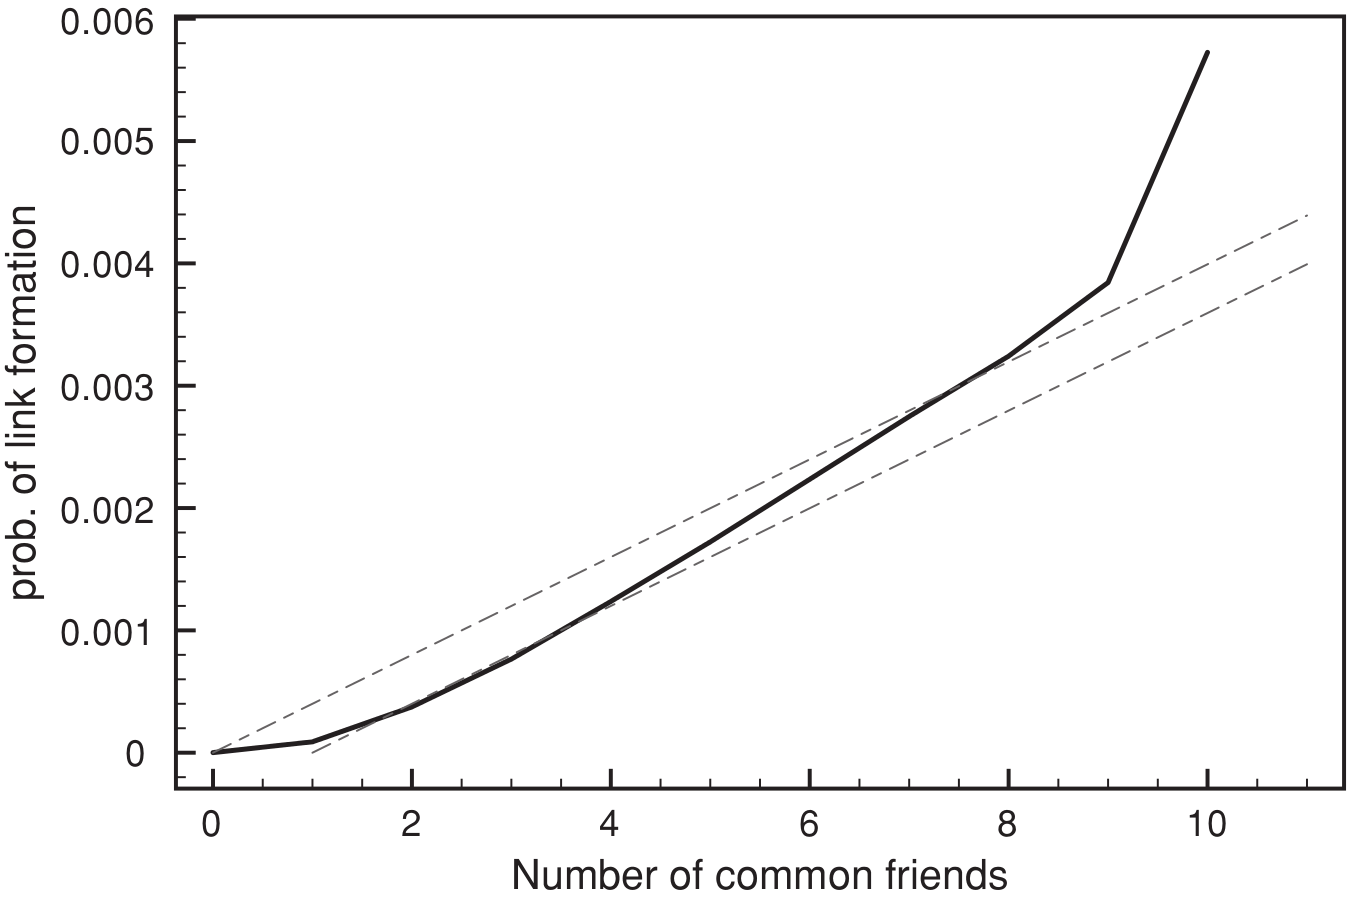
\includegraphics[width=0.8\linewidth]{images/21_emailFriends.png}
    \caption{Quantification des effets de la fermeture triadique dans un
        ensemble d'emails. La courbe déterminée à partir des données est
        une ligne noire continue. Les lignes en pointillés montrent la
        comparaison avec les probabilités depuis deux modèles simples
        dans lesquels les amis en communs fournissent des probabilités
    indépendantes de formation de lien}
    \label{emailFriends}
\end{figure}

On voit sur la figure \ref{emailFriends} (fermeture triadique) que la probabilité qu'un lien se forme augmente exponentiellement avec le nombre d'amis en commun.

\paragraph{Attention !}
Le comportement et donc les calculs sont différents pour la fermeture focale et d'adhésion !

\begin{figure}[!ht]
    \centering
    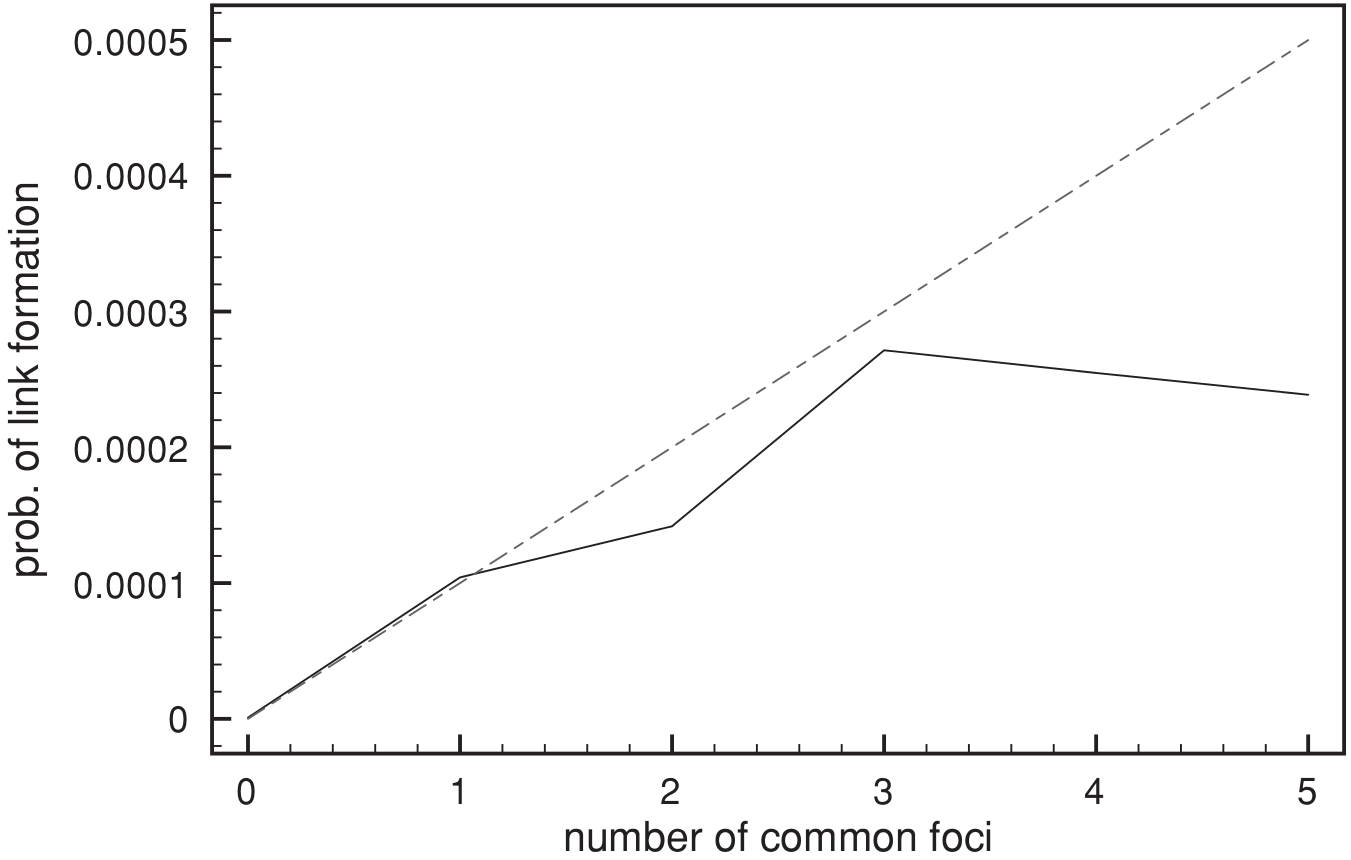
\includegraphics[width=\textwidth]{images/21_pointsCommuns.png}
    \caption{Quantification des effets d'une fermeture focalse dans un
        ensemble d'emails. A nouveau, la courbe déterminée à partir des
        données est une ligne continue, alors que la ligne en pointillés
    fournit une comparaison par rapport à une base simple.}
    \label{pointsCommuns}
\end{figure}

La figure \ref{pointsCommuns} (fermeture focale) nous montre que dans le cas où l'on considère le nombre d'intérêts en commun (ici, des cours), on arrive à un certains moment à saturation. Augmenter le nombre de points d'intérêts communs n'augmente plus la probabilité de création d'un lien à partir d'un certain point (ici 3 cours en communs).

\begin{figure}[!ht]
    \centering
    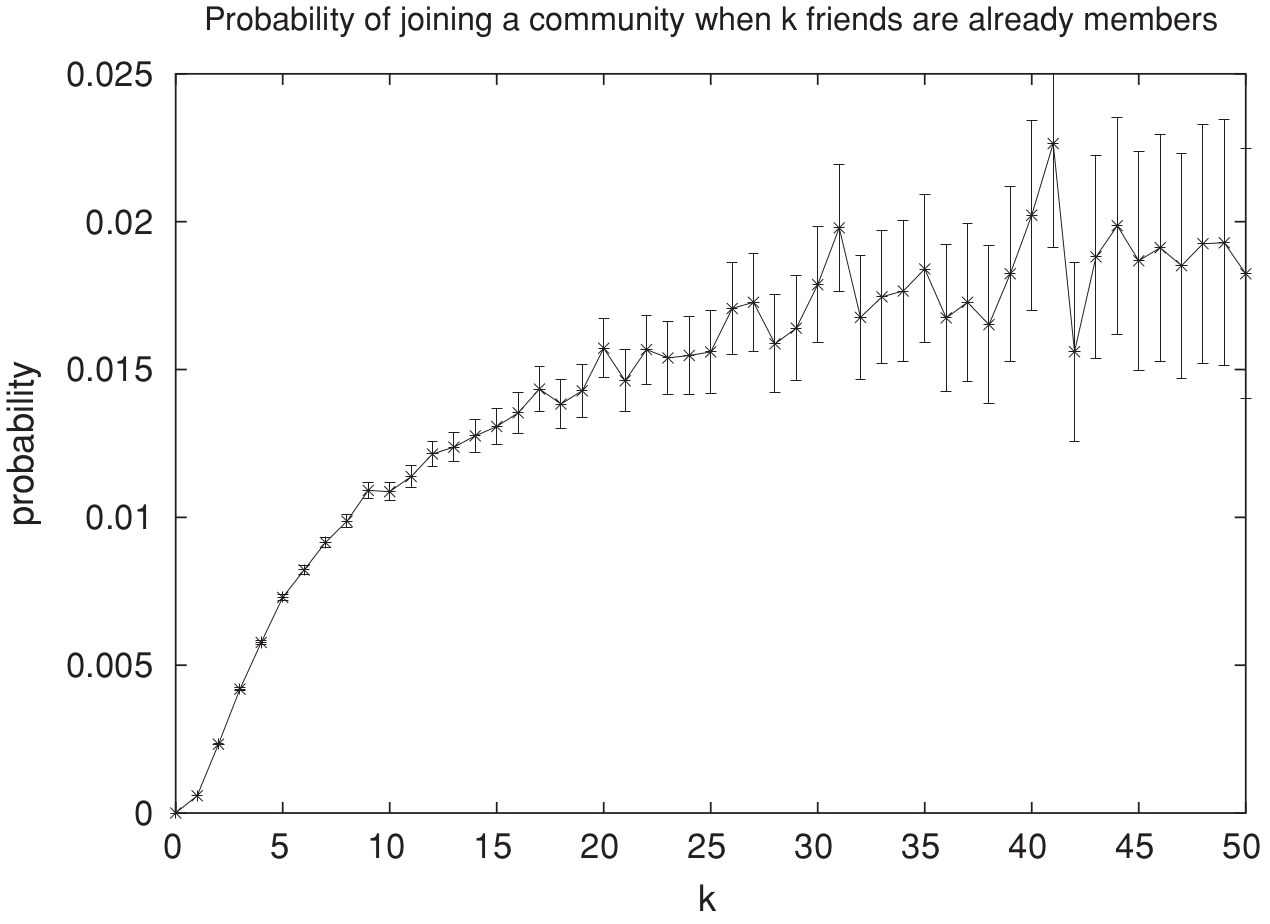
\includegraphics[width=\textwidth]{images/21_community.png}
    \caption{Quantification des effets de la fermeture d'adhésion dans
        un large ensemble de données en ligne : Le graphe montre la
        probabilité de rejoindre une communauté LiveJournal en fonction
    du nombre d'amis qui sont déjà membres.}
    \label{community}
\end{figure}

Enfin, la figure \ref{community} (fermeture d'adhésion) présente aussi un saturation à partir d'un certains nombre d'amis qui ont le même point d'intérêt.

\clearpage

\section{Quantifier les rôles relatifs de sélection d'influence sociale}
Les mécanismes de similitude :
\begin{itemize}
\item La sélection (intérieur, c'est nous qui faisons le choix)
\item L'influence sociale (extérieur, c'est les autres qui nous influencent) 
\end{itemize}
\subsection{Comment quantifier cela ?}

\paragraph{Exemple - Wikipédia}
Il peut exister une similitude de comportement entre rédacteurs. Par exemple les articles sur lesquels ils travaillent.

Raisonnement :
\begin{itemize}
\item On a des rédacteurs
\item Un lien entre deux rédacteurs : ils communiquent par la "Talk page" (chaque article a une "Talk page"). Autrement dit, si un rédacteur B communique sur la page de A, alors il y a un lien.
\item Les "points d'intérêts" ici sont les articles.
\item Quantification de la similitude
	$$\displaystyle\frac{\mbox{nombre d'articles rédigés par A ET B}}{\mbox{nombre d'articles rédigés par A OU B}}$$
Notons dès lors que la similitude ne peut pas être plus petite que 0 ni plus grand que 1. $0 \leq sim \leq 1$
\item Le moment de rupture est le moment où le lien est créé.
\item On compare la similitude avant et après cette rupture (figure
    \ref{wikipedia}). C'est surtout la sélection qui joue avant, car chaque rédacteur choisit ce qu'il doit ajouter ou modifier par rapport à ce qu'a mis l'autre rédacteur. Après la rupture, c'est principalement l'influence sociale qui entre en jeu car les deux rédacteurs mettent leurs idées en commun. %TODO utiliser plus la figure 4.13 pour cet exemple
\end{itemize}

\begin{figure}[!ht]
    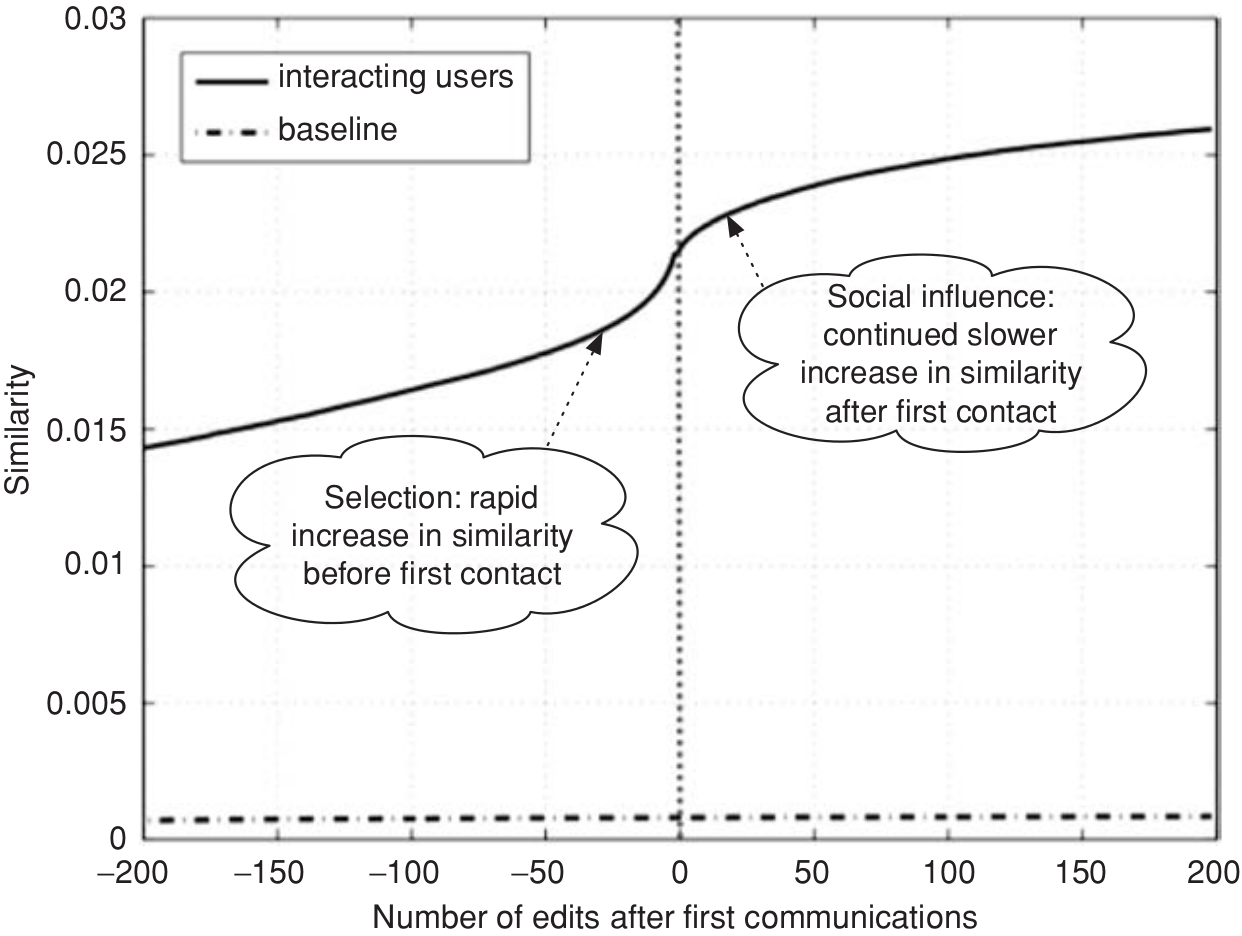
\includegraphics[width=\textwidth]{images/21_wikipedia.png}
    \caption{La similitude moyenne de deux contributeurs sur Wikipedia,
        relativement au temps (0) auquel ils ont communiqué pour la
        première fois. Le temps en abscisses, mesurés en unités
        discrètes correspond à une action Wikipedia faite par un des
        deux contributeurs. La courbe croît avant et après leur contact
        au temps 0, indiquant qu'à la fois la sélection et l'influence
        sociale joue un rôle ; la croissance de la similitude est plus
    forte juste avant le temps 0.}
    \label{wikipedia}
\end{figure}

  \section{Les relations positives et négatives}

Précédemment, les relations étudiées étaient considérées comme uniquement positives (on ne peut se faire que des amis). 

\includegraphics[scale=1]{images/22_force-positive}

Dans ce chapitre, nous allons étudier les graphes comportant également des relations positives et des relations négatives (on peut se faire des amis et des ennemis).

\includegraphics[scale=1]{images/22_amis-ennemis3.png}

\subsection{Théorie de l'équilibre de structure (Équilibre structurel fort)}
L'équilibre dans une structure va nous permettre d'identifier les situations stables et celles qui sont instables. Cette étude se fera dans un graphe complet (un graphe dont chaque paire a un lien et dont chaque lien peut être de type "+" ou "-").

\paragraph{}
L'idée cruciale est d'identifier dans le graphe les situations équilibrées et les situations qui ne le sont pas et qui engendrent un stress entre les nœuds.  

\begin{figure}[h!]
	\centering
	\includegraphics[width=\textwidth]{images/22_situation.png}
	\caption{Relations équilibrées et non équilibrées}
    \label{equi}
\end{figure}


Dans la figure \ref{equi}, les schémas de gauche sont considérés comme équilibrés. En effet, soit A, B et C sont tous amis et il n'y aucun conflit entre eux, soit B et C sont amis, mais sont en confit avec A. 

\paragraph{}
Par contre, les schémas de droite sont des situations non équilibrées. Dans la 3, B et C sont amis avec A mais ennemis entre eux, on peut supposer que A doive alors choisir un camp. La 4 indique que tous sont ennemis, mais il est fort probable que le graphe évolue vers une situation où deux nœuds se liguent contre le troisième. 

\paragraph{}
 
 On peut maintenant généraliser cela pour un nombre quelconque de nœuds. Ainsi un graphe complet sera fortement équilibré si chaque ensemble de 3 nœuds est équilibré et donc possède des liens de type $+++$ ou $+--$.   

\begin{figure}[h!]
	\centering
	\includegraphics[width=0.5\textwidth]{images/22_situation2.png}
	\label{equi2}
	\caption{Généralisation des relations équilibrées et non équilibrées}
\end{figure}

\paragraph{}
Si un graphe n'est pas équilibré, il a tendance à s'équilibrer. 


\subsection{Caractérisation de l'équilibre structurel} 
Dans le point précédent, nous avons réalisé une définition avec des conditions locales, mais il est difficile de comprendre ce que cela fait pour tout le graphe.
Ainsi nous voudrions une définition globale (une caractérisation) sur l'ensemble du graphe.




\subsubsection*{Preuve:}
Pour prouver qu'un graphe est bien équilibré, il faut pouvoir démontrer dans les deux sens :
\begin{enumerate}

\item $\Rightarrow$ la structure est équilibrée 
$\rightarrow$ direction facile à déterminer
%% pas sur du tout!!!!!
\item $\Leftarrow$ équilibrée est la structure 
$\rightarrow$ direction plus complexe à déterminer

\end{enumerate}

\subsection{Théorème d'équilibre [Frank Harary 1953]}

\begin{figure}[!ht]
	\centering
	\includegraphics[width=0.5\textwidth]{images/22_amis-ennemies2.png}
	\caption{2 groupes d'amis qui sont ennemis entre eux.}
    \label{groupami}
\end{figure}

Si un graphe complet est équilibré, alors:

\begin{enumerate}
	\item toutes les paires sont amies
	\item on peut diviser les nœuds en deux groupes X et Y, tel que X et Y chacun contient des amis mutuels et chaque membre de X est ennemi de chaque membre de Y comme représenté à la figure : \ref{groupami}.
\end{enumerate}

\subsubsection*{Preuve}

\begin{itemize}\renewcommand\labelitemi{\textbullet}
	\item graphe complet, annoté $+,-$
	\item graphe équilibré
	
	\begin{enumerate}
		\item si aucun lien négatif: forcément vrai car tous les triangles sont $+++$
		\item sinon il existe un lien négatif
	\end{enumerate}

	\item prenons un nœud A quelconque
	\item Définissons:

	\begin{enumerate}
		\item $X = $ A et tous ses amis
		\item $Y = $ les ennemis de A
	\end{enumerate}

	\item Est-ce que X et Y satisfont la condition du théorème?
\end{itemize}

\textit{À démontrer}

\begin{enumerate}
	\item chaque paire dans X = amis
	\item chaque paire dans Y = amis
	\item chaque nœud de X est ennemi de chaque nœud de Y
\end{enumerate}

\begin{figure}[!h]
	\centering
	\includegraphics[scale=1]{images/22_amis-ennemies.png}
\end{figure}

\subsubsection*{Exemple 1}

On peut retrouver ce type de comportement de graphe dans les relations internationales : lors de la séparation du Bangladesh au Pakistan en 1972, on a assisté à un surprenant soutien des États-Unis pour le Pakistan alors que celui-ci n'était pas un allié des Américains. 
\paragraph{Explication} 
Comme indiqué dans la figure \ref{paysconflit}, les USA désiraient se rapprocher de la Chine, pour y arriver, ils ont analysé les relations des différents pays de la région. Ils ont ainsi constaté que la Chine avait des ennemis communs avec le Pakistan. Un rapprochement avec le Pakistan lui permettait de rentrer dans le groupe des amis de la Chine.


\begin{figure}[h!]
	\centering
	\includegraphics[scale=1]{images/22_pays-conflit.png}
	\label{paysconflit}
	\caption{Relation lors de l'indépendance du Bangladesh}
\end{figure}

\paragraph{}
Une autre approche de ce conflit peut être réalisée d'un point de vue de la Chine : 

\begin{itemize}
	\item Vietnam du Nord $\overset{+}{\longleftrightarrow}$ Inde
	\item Pakistan $\overset{-}{\longleftrightarrow}$ pays du bloc EST
	\item Chine : vote l'abolition du Bangladesh à l'ONU
\end{itemize}
%TODO besoin de plus d'explications ici

\subsubsection*{Exemple 2}
Un autre exemple de ce jeu diplomatique est donné à la figure 55 du livre de référence et représente le jeu des alliances des grandes puissances européennes à la veille de la Première Guerre mondiale.

On assiste à un équilibrage du graphe des relations avec des pays qui changent continuellement d'alliés jusqu'au moment de la triple entente et de la triple alliance qui sépara tous les pays d'Europe en deux camps ennemis.
%TODO ajouter illustration

\subsubsection*{Exemple 3}
Dans ce troisième exemple, on touche directement les réseaux sociaux où il existe des relations \textit{Like} ou \textit{Trust} et \textit{Dislike} ou \textit{Distrust} dont les utilisateurs peuvent se servir pour juger le contenu des autres (par exemple Reddit, les reviews sur Amazon...)

Le classement de produits y est libre: un utilisateur est libre d'avoir des opinions positives (+) ou négatives (-) sur les autres

\begin{figure}[!h]
	\centering
	\includegraphics[scale=1]{images/22_graphe-oriente.png}
\end{figure}

\subsubsection*{Transitivité}  

Il est intéressant de savoir si les relations sont transitives ou non, autrement dit si A croit en B et que B croit en C, A croira-t-il en C?
\begin{align*}
A \overset{trust}{\longrightarrow} B \overset{trust}{\longrightarrow} C \overset{?}{\Longrightarrow} A \overset{trust}{\longrightarrow} C
\end{align*}

Ou alors, si A n'a pas confiance en B et que B n'a pas confiance en C, est-ce que A aura alors confiance en C ou non?


\begin{align*}
A \overset{distrust}{\longrightarrow} B \overset{distrust}{\longrightarrow} C \overset{?}{\Longrightarrow} &A \overset{trust}{\longrightarrow} C\\
&A \overset{distrust}{\longrightarrow} C
\end{align*}

Finalement, tout est possible selon le cas rencontré : 
\begin{itemize}
\item Si le trust signifie une relation d'amitié, la transitivité sera respectée. 
\item Si le trust indique une confiance sur l’opinion, la transitivité ne peut être respectée. 
\item Si par contre trust en une proximité dans les opinions politiques, un rapprochement de A et C est probable. 
\end{itemize}


\paragraph{Conclusion :}La théorie de l'équilibre structurel sera gérée selon le cas




\subsection{Équilibre structurel faible}
L'équilibre structurel faible, à l'instar de l'équilibre structurel fort, se base sur la
notion de stabilité des triangles du graphe. Mais contrairement à l'équilibre fort, on ajoute deux cas instables   

\begin{figure}[!h]
	\centering
	\includegraphics[scale=1]{images/22_Instabilite.png}
\end{figure}

Un graphe complet annoté est faiblement équilibré si:
\begin{itemize}
\item aucun triplet n'est $++-$;
\item tous les triplets sont de type $+++, +--, ---$. 
\end{itemize}
\paragraph{}
L'équilibre faible permet une structure \textbf{multipolaire}.

\begin{figure}[h!]
	\centering
	\includegraphics[scale=1]{images/22_etoile-amis.png}
	\label{fig:multipolaire}
	\caption{Structure multipolaire}
\end{figure}



\subsubsection*{Théorème d'équilibre pour l'équilibre faible}

Si graphe complet annoté est faiblement équilibré, alors on peut diviser ses nœuds en groupes :

\begin{itemize}


\item dans un groupe: amis

\item autre groupe: ennemis

\end{itemize}

\paragraph{Preuve : } \textit{(analogue à la preuve sur l'équilibre structurel)}


\begin{enumerate}

\item Nœud A + tous ses amis appartiennent au groupe X \\
$\to$ amis mutuels, car ($+++$).

\item A $+$ ses amis sont ennemis avec tous les autres.

\item Enlever A $+$ ses amis : nouveau graphe.\\
$\to$ raisonnement récursif

\end{enumerate}

  \chapter{Structure du Web} %chapitre 13


\section{Mémoire associative - Hypertexte}

Liens hypertextes : chaque élément a des liens vers et depuis d'autres éléments. Un contenu hypertexte est un contenu auquel il est fait référence dans un document.

\vspace{0.5cm}
Deux exemples de contenus hypertextes :

$
\left. 
%\text{
\parbox{0.5\linewidth}{
\begin{itemize}
\item \textbf{Graphe de citations} \\
		Précurseur du web : nœuds indépendants, liens strictement vers le passé
\item \textbf{Encyclopédie} \\
		Les articles renvoient vers d'autres articles \\ (Wikipédia)
\end{itemize}
}%}
\hspace{0.5cm} \right\}
$ Réseaux d'informations




\begin{figure}[!h]
	\centering
	\includegraphics[scale=0.75]{images/23_image1.png}
	\caption{Liens hypertexte vers des articles}
	\label{hypertexte}
\end{figure}

\textbf{Problème de cohérence}

\begin{itemize}
\item \underline{Web}: Cohérence \textit{"a posteriori"} 
						\vspace{0.1cm}
                       \\ Le web n'ayant pas d'organisation, on va devoir en trouver une : un index ou un moteur de recherche
                       \vspace{0.2cm}
      
\item \underline{Wikipedia}: Cohérence \textit{"a priori"}
							\vspace{0.1cm}
                             \\ Une structure existe déjà, définie par les rédacteurs, les modérateurs et les règles de structure.
\end{itemize}

Le succès du Web réside dans la possibilité de trouver une structure \textit{a posteriori} à ce dernier, notamment grâce à l'algorithme PageRank. Altavista, Google, Lycos, ... proposent tous leur version de moteur de recherche. C'est grâce à l'efficacité de PageRank que Google s'est imposé largement comme moteur de recherche dominant.

\section{Le Web est un graphe orienté}
\begin{itemize}
\item \underline{Chemin dans un graphe orienté}: A $- \rightarrow$ B
\vspace{0.1cm}
\\Séquence de nœuds qui commence avec A et termine avec B et où chaque paire consécutive correspond à un lien orienté.

\item \underline{Connectivité}: 
\vspace{0.1cm}
\\Un graphe orienté est connexe s'il existe un chemin orienté entre chaque paire de nœuds.
\end{itemize}

\section{Composant fortement connexe (CFC) \\ \textit{Strongly Connected Component (SCC)} }

À l'intérieur d'un graphe orienté, un composant fortement connexe est :
\begin{itemize}
    \item Un ensemble de nœuds tel qu'il existe un chemin orienté entre chaque paire.
    \item L'ensemble ne fait pas partie d'un plus grand environnement ayant la même propriété. 
\end{itemize}

\begin{figure}[!ht]
\centering
\includegraphics[scale=0.3]{images/23_fig13-6.png}
\caption{Un graphe dirigé avec ses CFCs identifiés}
\label{cfc_exemple}
\end{figure}

Les CFCs forment un genre de \textit{"super noeud"}. Pour la connectivité, on peut ignorer la structure interne des CFCs.

\vspace{0.3cm}

On peut donc transformer le graphe en un graphe réduit : le CFC devient un unique nœud. Pour trouver qu'un chemin existe dans le graphe original, il suffit de trouver un chemin dans le graphe réduit.
Un exemple de transformation de ce type est illustré sur la figure \ref{cfc_transformation}.
\vspace{0.3cm}

\begin{figure}[!ht]
\centering
\includegraphics[width=0.85\linewidth]{images/23_schema2.png}
\caption{Exemple de transformation du graphe}
\label{cfc_transformation}
\end{figure}


\section{Web en nœud papillon (\textit{$\approx$ années 2000})}
	Maintenant, à quoi ressemble le graphe réduit du web ? Autour des années 2000, sa structure était proche de celle d'un nœud papillon, tel que celui représenté sur la figure \ref{noeud_papillon}.
	
	On repère trois composants principaux :
	\begin{itemize}
	\item Un composant "in", qui contient des liens hypertextes sortants.
	\item Un composant fortement connecté principal, qui forme un "noyau".
	\item Un composant "out", qui contient beaucoup de liens hypertextes entrants.
	\end{itemize}
	
	\begin{figure}[!ht]
		\centering
		\includegraphics[scale=0.25]{images/23_fig13-7.png}
		\caption{Structure en nœud papillon du web}
		\label{noeud_papillon}
	\end{figure}

\section{Émergence du Web 2.0 (\textit{$\ge$ années 2000})}
L'émergence du Web 2.0 se déroule entre 2000 et 2010. Il s'agit en fait d'un changement d'attitude général des certains acteurs importants du web conduisant à une structuration de la toile basée sur trois grands principes. 
\begin{enumerate}
    \item \underline{Création collaborative} de contenu plutôt que des pages personnelles.
    \item \underline{Services} vers lesquels sont transférés les données personnelles. Au lieu de publier du contenu  sur des sites personnels, les gens se tournent vers des services pour publier leur contenu (par exemple YouTube, Flicker, Github...)
    \item \underline{Personnes} au lieu des documents. On n'identifie plus un document en fonction de son contenu, mais en fonction de son auteur ou de la personne qui en est le sujet.
\end{enumerate} 

\vspace{0.3cm}
%\begin{minipage}{15cm}
\textbf{Technologies utilisées:}
    \begin{itemize}
        \item Blogs (Skyblog), ensuite détrônés par les réseaux sociaux (Facebook, Twitter, MySpace, Friendster...)
        \item Deep Web : création de page à la demande (créer un nouveau profil, une page Wikipédia, un groupe d'intérêt...)
        \item Cloud : regroupement et partage de ressources "à la demande", permet plus d'élasticité (adaptation en fonction des besoins)
    \end{itemize}
%\end{minipage}

\vspace{0.5cm}

\begin{framed}
    \textbf{Un petit bout d'histoire}
    
    \vspace{0.3cm}
    
    \underline{Quelques précurseurs} :
    
    \begin{itemize}
        \item \underline{1945 - Vannevar Bush} : Conseiller du président des États-Unis, Roosevelt\\ 
        Il a écrit un article intitulé "As We May Think" dans lequel il explique son appareil électronique relié à une bibliothèque et capable d'afficher des livres et de projeter des films appelé "Memex".
        \item \underline{1934 - Paul Otlet} : Documentaliste\\ 
        Il avait imaginé un système où l'on pourrait faire des recherches et consulter le résultat de ces recherches sur un écran. Cette intuition d'un pré internet est à l'origine d'une structuration des ressources des bibliothèques. Il est aussi un pionnier des microfiches, des fiches indépendantes qui stockent des informations, ayant une ressemblance non négligeable avec les pages web d'aujourd'hui.
        \item \underline{1990 - Tim Berners-Lee et  Robert Cailliau - CERN} : Inventeur du World Wide Web\\
        Ils se sont inspirés des écrits de Vannevar Bush pour inventer le WWW, avec sa structure de pages indépendantes reliées par des liens hypertextes.
    \end{itemize}
\end{framed}    
\vspace{0.5cm}


\chapter{Recherche dans le Web} %chapitre 14
Comment trouver une information ?
\vspace{0.3cm}

\underline{1960} : Concept de mot-clé $\rightarrow$ Limitations fortes

\begin{itemize}
    \item Limitations dues au concept de mot
        \begin{itemize}
            \item Synonymie : plusieurs mots pour le même concept.
            \item Polysémie : un mot pour plusieurs concepts.\\
            Par exemple les noms propres peuvent référer à plusieurs personnes, des lieux et des organisations.

        \end{itemize}
        
        Autrement dit, il n'y a pas de bijection entre les mots et les concepts.
        
    \item Limitations dues à l'abondance d'informations. \vspace*{0.2cm} \\
    $\left. %\text{
    \parbox{0.5\linewidth}{
        \begin{itemize}
            \item \underline{Avant}: Les informations sur le web étaient rares. 
            \item \underline{Maintenant}: Il y a beaucoup trop d'informations.
        \end{itemize}
        %}
        } \hspace{0.5cm} \right 
        \}
        $ Plus grand problème du web
\end{itemize}
    
	Pour résoudre le problème de surabondance d'informations, il faut trouver une façon de savoir quelle page est la meilleure. Comment faire ce choix ?
	
	La meilleure solution est d'utiliser l'information contenue dans la structure du réseau.

  \section{L'analyse des liens}
\begin{itemize}
\item Concentrateurs (\textit{Hubs})
\item Autorités (\textit{Authorities})
\item Comment trouver la meilleure page ? (Voir figure \ref{fig-14-1}	)
\end{itemize}



\begin{figure}[!ht]
\centering
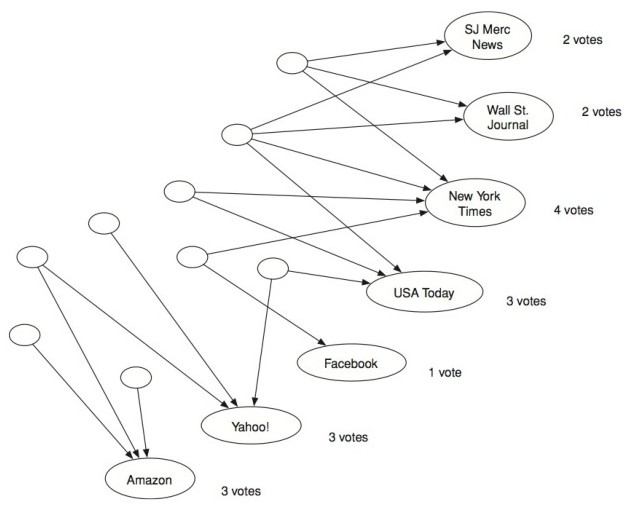
\includegraphics[width=0.8\linewidth]{images/ref/fig-14-1.jpeg}
\caption{Comptage des liens entrants pour la recherche "newspapers"}
\label{fig-14-1}
\end{figure}

\subsection*{Requête "newspapers"}

\paragraph{Pourquoi Facebook, Yahoo, Amazon, se retrouvent-ils dans la requette News Papers ?}
Car beaucoup d'utilisateurs ont des pages concentrées sur ces sites et comme dans cet exemple on utilise un algorithme qui n'est pas très sophistiqué, elles apparaissent. 

\paragraph{Comment trouver la meilleure page ?}
\begin{enumerate}
\item Compter les liens entrants comme une estimateur de la qualité d'une autorité.
\item Classer les concentrateurs en fonction de la qualité des pages qu'elles référencent.
\item Mettre à jour la qualité des autorités en fonction du poids de la source des liens.
\item Mettre à jour les concentrateurs.
\end{enumerate}

\subsubsection{Algorithme}

\begin{itemize}
\item Pages autorité (liens entrants) $ \rightarrow $ auto (p)
\item Pages concentrateurs (liens sortants) $ \rightarrow $ conc (p)
\item Mises à jour des liens entrants:
\begin{align*}
 auto'(p) =   \sum_ {p'\rightarrow p}conc(p') &&
\text{\emph{avec $p'\rightarrow p $ les pages p' qui ont un lien vers P}}
\end{align*}

\item Mises à jour des liens sortants: 
\begin{align*}
conc'(p) = \sum_ {p\rightarrow p'}auto(p') &&
\text{\emph{avec $p \rightarrow p' $ les pages p' qui sont référencées par p}} 
\end{align*}

\end{itemize}



\subsubsection*{Itération}}

$$
\forall~p~in~pages :
\left \{
\begin{array}{l}
auto(p) = 1 \\
conc (p) = 1 

\end{array}
\right.
$$

 Mise à jour, normalisation :
 
 \begin{align*}
 auto'(p) = \frac{auto (p)}{\sum auto(p')}
 \end{align*}
 \begin{align*}
 conc' (p) = \frac{conc (p)}{\sum conc(p)}
 \end{align*}
 Cet algorithme converge


En appliquant maintenant cet algorithme, la requête "newspapers" nous donnerait les résultats suivants (\ref{pageRankNews1} et \ref{pageRankNews2}):


\begin{figure}[!ht]
\centering
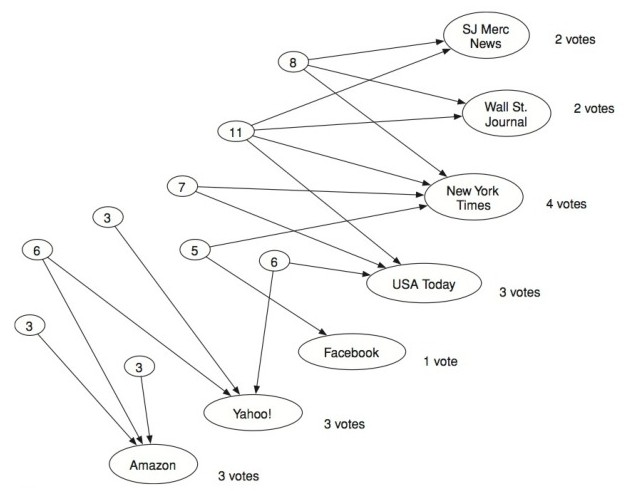
\includegraphics[width=0.8\linewidth]{images/ref/fig-14-2.jpeg}
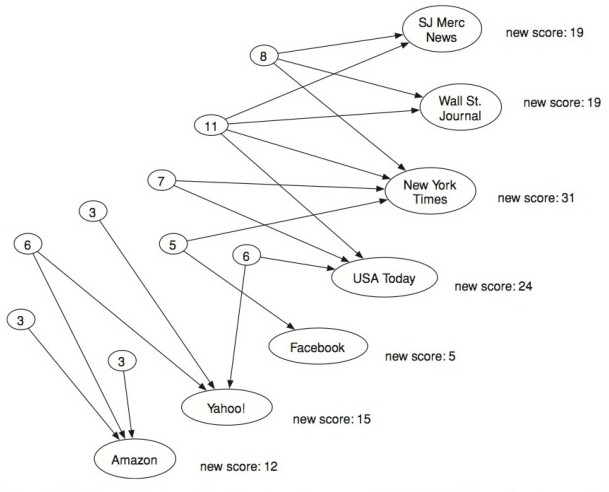
\includegraphics[width=0.8\linewidth]{images/ref/fig-14-3.jpeg}
\caption{Page Rank}
\label{pageRankNews1}
\end{figure}

\begin{figure}[!ht]
\centering

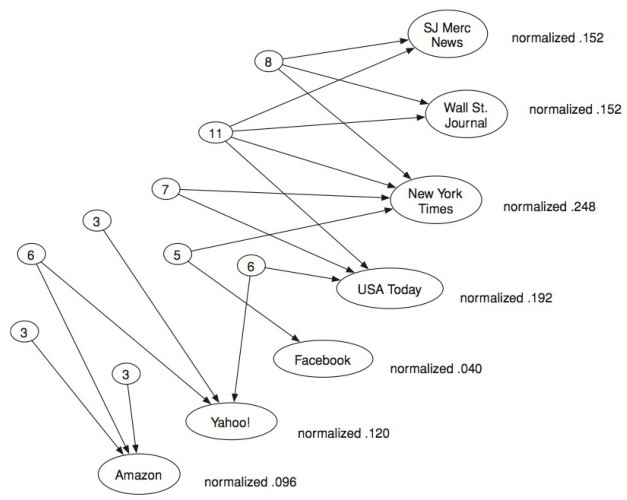
\includegraphics[width=0.8\linewidth]{images/ref/fig-14-4.jpeg}
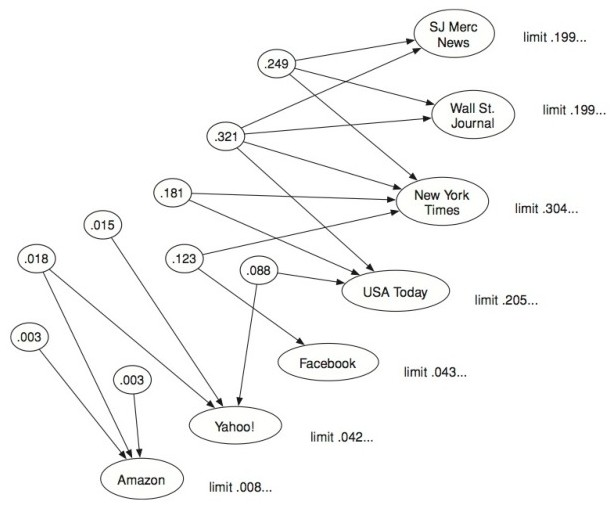
\includegraphics[width=0.8\linewidth]{images/ref/fig-14-5.jpeg}
\caption{Page Rank}
\label{pageRankNews2}
\end{figure}



\newpage

	
Comme nous pouvons voir, l'algorithme compte le nombre de liens entrants pour attribuer un poids à chaque place. Puis on normalise les valeurs trouvées, ce qui correspond au poids de la page.
Au plus grand est le poids d'une page au plus son autorité sera grande.

\section{PageRank}
\begin{itemize}
	\item Consolider autorités et concentrateurs.
	\item Une valeur par nœud : son "PageRank" que nous allons calculer. 
	\item Intuition: Un "fluide" qui circule dans le réseau. 
\end{itemize}

\textbf{ Algorithme PageRank :}
\begin{enumerate}
	\item N noeuds (chaque noeud représentant une page) :
	Initialisation Pr(p) =  $\frac{1}{n}$
	\item Choisir un nombre de pas k
	\item K mises à jour:\\
	Pr(p) = $ \sum_ {p'}\frac{Pr(p')}{n(p')} $ avec n(p') le nombre de liens sortant de p' et Pr(p') le poids (ou PageRank) de p' à la $k^{ème}$ itération.
\end{enumerate}
\subsection*{Exemple de PageRank :}

\begin{figure}[!ht]
\centering
 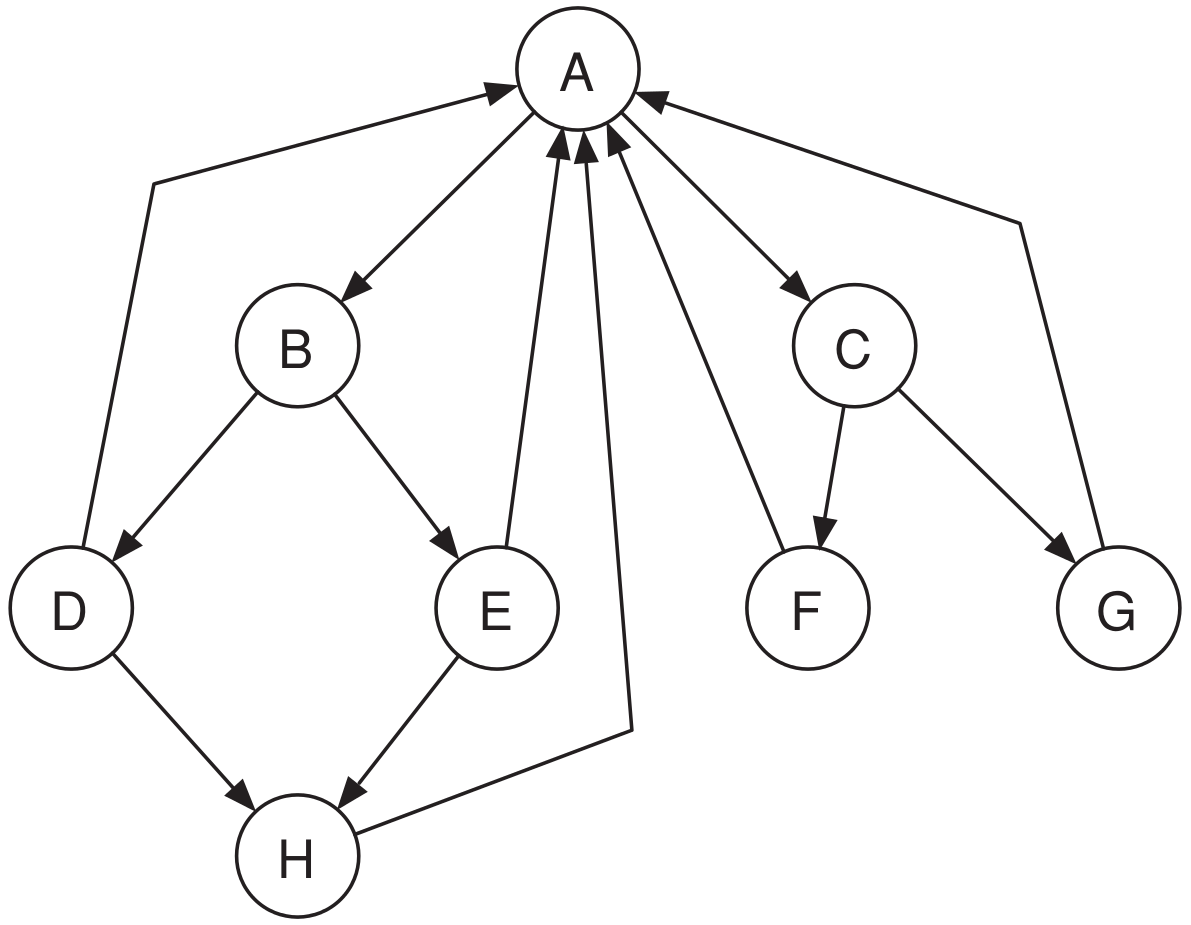
\includegraphics[width=0.5\linewidth]{images/24_PageRank.png}
 \caption{Un ensemble de huit pages : la page A a le plus large
     PageRank, suivies par les pages B et C (qui collectent l'appui de
 A)}
 \label{graphPageRank}
\end{figure}

 
 	\begin{tabular}{|c| c |c |c |}
		\hline
		Noeuds/Itérations & 0 & 1 & 2 \\
		\hline
		A & 1/8 & 1/2 & 5/16 \\
		B & 1/8 & 1/16 &  1/4   \\
		C & 1/8 & 1/16 & 1/4    \\
		D & 1/8 & 1/16 & 1/32  \\
		E & 1/8 & 1/16 &  1/32   \\
		F & 1/8 & 1/16 & 1/32    \\
		G & 1/8 & 1/16 & 1/32    \\
		H & 1/8 & 1/8 &  1/16   \\
		\hline
		$\sum $ & 1 & 1 & 1 \\
		\hline
	\end{tabular}

Par exemple, A a un PageRank de $\frac{1}{2}$ après la première mise à
jour car il reçoit les PageRanks de F, G, H ainis que la moitié de D et
E. D'autre part, B et C reçoivent chacun la moitié du PageRank de A,
donc ils ont seulement $\frac{1}{16}$ chacun dans la première étape.
Mais une fois que A a reçu beaucoup de PageRank, B et C en profite dans
l'étape suivante. Intuitivement, cela s'explique par le fait que si on
considère A comme était une page importante, les liens qui la composent
doivent l'être eux aussi.

 Si nous continuons à laisser travailler l'algorithme, pour un nombre n fini d'itérations telles que k=n, il y aura convergence de l'algorithme. Dans cet exemple-ci,  nous aurons :

	$$Pr(A) = 4/13 ; Pr(B) = 2/13 ; Pr(C) = 2/13 ; Pr(Autres) = 1/13$$
 
Et la condition $\sum Pr(p) = 1$ est toujours vérifiée.
 
 L'équilibre est vérifié si le graphe est connexe,par contre si il ne
 l'est pas un problème se pose: Le fluide peut arriver au mauvais noeud
 (Par analogie avec un réseau d'eau, on comprend que ce genre de
 situation entraîne un blocage du \og{}fluide\fg{}) :

\begin{figure}[!ht]
    \centering
    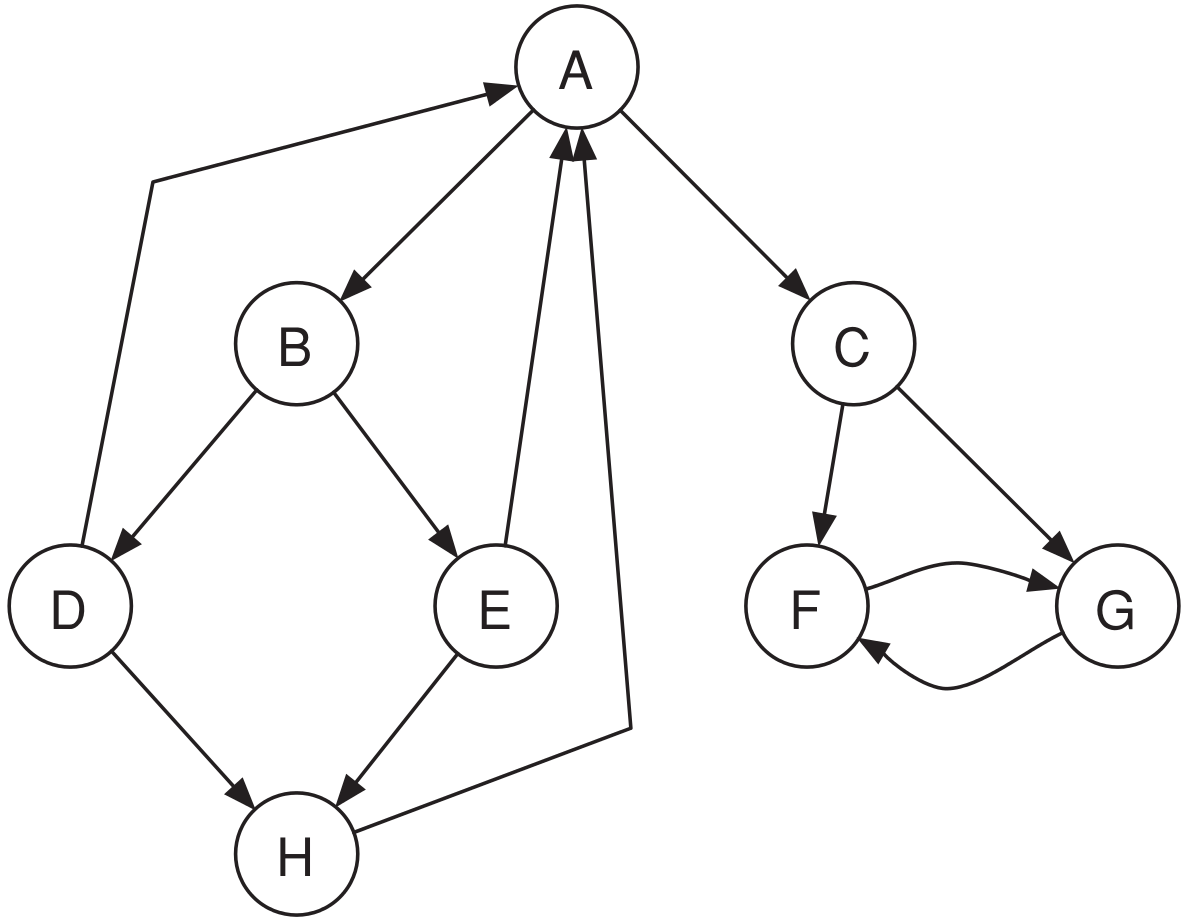
\includegraphics[width=0.7\linewidth]{images/24_PageRank_non_connexe.png}
    \caption{Le même ensemble de huit pages, mais F et G ont changé
        leurs liens pour pointer l'un vers l'autre. Sans un effet de
    lissage, tout le PageRank irait vers F et G.}
\end{figure}

\subsection*{Solution du problème}
	La solution dans le cas où le PageRank s'amasse dans un n\oe ud serait de former des cycles afin d'assurer que le fluide continue à circuler.
	
 	En pratique, on va réinjecter un peu de fluide partout à chaque itération pour éviter que le fluide se concentre dans les nœuds qui n'ont que des liens entrants et pas de liens sortant. De cette façon on referme la boucle et le fluide peut continuer à circuler.
 	
 	Cela peut s'apparenter à la circulation de l'eau dans l'atmosphère : le fluide s'évapore un peu partout et retombe de façon équitable.

	Ancienne règle de mise à jour :
	\begin{align*}
	Pr(p) =  \sum_ {p'}\frac{Pr(p')}{n(p')}
	\end{align*}
	
 	Nouvelle règle de mise à jour : \\
	\begin{align*}
         Pr(p) = S*Pr(p) + (1-S)  \times \frac{1}{n} \\
	 \text{Où S est un paramètre : $ 0 \le S \le 1 $} 
	\end{align*}
        
\subsection*{ Une autre manière de voir l'algorithme:}
    Cet algorithme correspond aussi au comportement des utilisateurs sur le web. La marche aléatoire d'un utilisateur sur le web peut être vue comme : 
	\begin{itemize}
        \item Probabilité de S : Suivre un lien dans la page web ou l'on se trouve.
        \item (1-S) : Choisir un n\oe ud au hasard, par exemple, taper une URL et accéder directement à un site.
        \item Pr(p), tel que calculé dans la nouvelle règle de PageRank, est la probabilité de tomber sur la page p.
	\end{itemize}
	
\subsection*{Historique de PageRank}

	PageRank a commencé à être utilisée au début des années 1990, mais a été en partie abandonné à partir de 2003-2004 pour bloquer les services de SEO (\textit{Search Engine Optimisation}) et autres manipulations du système comme les Google bombs\footnote{wikipedia.org/wiki/Google\_bomb}.
	
	Ceux-ci consistent à altérer les résultats de recherche soit en créant de nombreuses pages contenant des liens vers une page en particulier, soit en utilisant de gros concentrateurs qui contiennent énormément de mots-clés.
	
	Outre les modifications à l'algorithme de tri, certains sites utilisent aussi un attribut html "\textit{nofollow}" qui a pour effet que ces liens n'entrent pas en compte dans le PageRank d'une page. C'est notamment utilisé par les sites de blogging et les sites collaboratifs comme les wikis afin que personne n'ait intérêt à saboter une page pour ajouter un lien et améliorer le classement d'un site en particulier.\footnote{wikipedia.org/wiki/Nofollow}


  % \include{concl}
  % \newpage
  \include{references}
\end{document}

